% Format teze zasnovan je na paketu memoir
% http://tug.ctan.org/macros/latex/contrib/memoir/memman.pdf ili
% http://texdoc.net/texmf-dist/doc/latex/memoir/memman.pdf
% 
% Prilikom zadavanja klase memoir, navedenim opcijama se podešava 
% veličina slova (12pt) i jednostrano štampanje (oneside).
% Ove parametre možete menjati samo ako pravite nezvanične verzije
% mastera za privatnu upotrebu (na primer, u b5 varijanti ima smisla 
% smanjiti 
\documentclass[12pt,oneside]{memoir} 

% Paket koji definiše sve specifičnosti master rada Matematičkog fakulteta
\usepackage[latinica]{matfmaster}

% Dodatni paketi

\usepackage{xcolor}

% Paket za prikazivanje C# koda
\usepackage{listings}

% paket za subfigure
\usepackage{caption}
\usepackage{subcaption}


\definecolor{bluekeywords}{rgb}{0,0,1}
\definecolor{greencomments}{rgb}{0,0.5,0}
\definecolor{redstrings}{rgb}{0.64,0.08,0.08}
\definecolor{xmlcomments}{rgb}{0.5,0.5,0.5}
\definecolor{types}{rgb}{0.17,0.57,0.68}

\lstset{language=[Sharp]C,
	captionpos=b,
	numbers=left,
	numberstyle=\tiny,
	frame=single,
	framesep=10pt,
	showspaces=false,
	showtabs=false,
	breaklines=true,
	showstringspaces=false,
	breakatwhitespace=true,
	tabsize=4,
	framexleftmargin=1.5em,
	xleftmargin=2em,
	escapeinside={(*@}{@*)},
	commentstyle=\color{greencomments},
	morekeywords={partial, var, value, get, set},
	keywordstyle=\color{bluekeywords},
	stringstyle=\color{redstrings},
	basicstyle=\ttfamily\footnotesize,
	classoffset=1, 
	morekeywords={ until, final, abstract, event, new, struct,
	as, explicit, null, switch,
	base, extern, object, this,
	bool, false, operator, throw,
	break, finally, out, true,
	byte, fixed, override, try,
	case, float, params, typeof,
	catch, for, private, uint,
	char, foreach, protected, ulong,
	checked, goto, public, unchecked,
	class, if, readonly, unsafe,
	const, implicit, ref, ushort,
	continue, in, return, using,
	decimal, int, sbyte, virtual,
	default, interface, sealed, volatile,
	delegate, internal, short, void,
	do, is, sizeof, while,
	double, lock, stackalloc,
	else, long, static,
	enum, namespace, string, begin,
	declare, function, algorithm, integer,
	procedure,
	>,<,.,;,,,-,!,=,~,
	await},
	classoffset=0,
}

\lstdefinestyle{yaml}{
     basicstyle=\color{blue}\footnotesize,
     rulecolor=\color{black},
     string=[s]{'}{'},
     stringstyle=\color{blue},
     comment=[l]{:},
     commentstyle=\color{black},
     morecomment=[l]{-}
 }


% Datoteka sa literaturom u BibTex tj. BibLaTeX/Biber formatu
\bib{references}

% Ime kandidata na srpskom jeziku (u odabranom pismu)
\autor{Milana Kovačević}
% Naslov teze na srpskom jeziku (u odabranom pismu)
\naslov{Razvoj platforme za distribuirano izračunavanje u oblaku}
% Godina u kojoj je teza predana komisiji
\godina{2022}
% Ime i afilijacija mentora (u odabranom pismu)
\mentor{prof. dr Saša \textsc{Malkov}\\ Univerzitet u Beogradu, Matematički fakultet}
% Ime i afilijacija prvog člana komisije (u odabranom pismu)
\komisijaA{prof. dr Filip \textsc{Marić}\\ Univerzitet u Beogradu, Matematički fakultet}
% Ime i afilijacija drugog člana komisije (u odabranom pismu)
\komisijaB{doc. dr Ivan \textsc{Čukić}\\ Univerzitet u Beogradu, Matematički fakultet}

% Datum odbrane (odkomentarisati narednu liniju i upisati datum odbrane ako je poznat)
% \datumodbrane{}

% Apstrakt na srpskom jeziku (u odabranom pismu)
\apstr{Distribuirani sistemi predstavljaju skup nezavisnih mašina, koje su međusobno povezane mrežom. Mašine međusobno sarađuju i raspoređuju poslove kako bi rešile zadati problem. Distribuirani sistemi za izračunavanje su specijalizovani za izvršavanje resursno zahtevnih zadataka koristeći visok nivo paralelizma koji se postiže raspodelom poslova na čvorove. Ovim se dostižu visoke performanse i mogućnost izvršavanja poslova koji često ne bi mogli da se izvrše na jednoj mašini.  Glavni čvor koordiniše izvršavanje, a ostali izvršavaju zadatke. Ovaj rad opisuje sistem za distribuirano izvršavanje poslova, nazvan DCS, implementiran u programskom jeziku C\#. Sistem DCS predstavlja Sofver kao servis rešenje za obradu poslova. Prednost sistema je njegova modularnost, jer ga je moguće proširiti i specijalizovati da izračunava različite poslove od interesa. U radu je fokus na infrastrukturi sistema. Predstavljena je njegova arhitektura kao i način organizovanja i izvršavanja poslova. Dodatno, predstavljen je i način njegovog pokretanja u okviru klastera Kubernetes, korišćenjem \emph{Docker} kontejnera. U okviru rada je predstavljano i pokretanje sistema DCS u oblaku, koristeći platformu Azure i servis Azure Kubernetes Service. DCS je integrisan sa ostalom infrastrukturom u oblaku, koristeći pomoćne servise za praćenje rada sistema i detekciju grešaka.}

% Ključne reči na srpskom jeziku (u odabranom pismu)
\kljucnereci{distribuirani sistemi, distribuirano izračunavanje, Azure tehnologije, oblak, Softver kao servis, Kubernetes, Docker}

\begin{document}
% ==============================================================================
% Uvodni deo teze
\frontmatter
% ==============================================================================
% Naslovna strana
\naslovna
% Strana sa podacima o mentoru i članovima komisije
\komisija
% Strana sa posvetom (u odabranom pismu)
\posveta{Porodici i najbližima \\ za strpljenje i podršku tokom studiranja}
% Strana sa podacima o disertaciji na srpskom jeziku
\apstrakt
% Sadržaj teze
\tableofcontents*

% ==============================================================================
% Glavni deo teze
\mainmatter
% ==============================================================================

% ------------------------------------------------------------------------------
\chapter{Uvod}
% ------------------------------------------------------------------------------

U uvodnom delu su ukratko dati pregled i opšte informacije o distribuiranim sistemima, kako bi se stekla šira slika o oblasti ovog rada. Opisani su osnovni pojmovi i dati primeri relevantnih postojećih sistema za distribuirano izračunavanje. U nastavku su opisane korišćene tehnologije i alati potrebni za razumevanje rada. Detalji realizacije praktičnog dela su opisani u poglavlju \ref{chp:sistemdcs}, gde su dati pregled funkcionalnosti, detalji implementacije, kao i način pokretanja sistema u oblaku i njegovog testiranja i praćenja. U poglavlju \ref{chp:rezultati}, opisani su rezultati implementiranog rešenja kroz primer i analizu performansi. Na kraju, predložena su moguća unapređenja sistema i pravci njegovog daljeg razvoja, kao i zaključak celokupnog rada.

\section{Distribuirani sistemi}

Distribuirani sistemi se sastoje od skupa fizički odvojenih mašina, tzv. čvorova, koje su međusobno povezane mrežom. Na ovim mašinama su pokrenute softverske jedinice koje međusobno dele odgovornost, poslove, komuniciraju i sinhronizuju se, kako bi rešile zadati problem.

Prednosti ovako struktuiranog softvera su značajne. Neke od njih su:
\begin{enumerate}
\item Postizanje visokog nivoa paralelizacije prilikom raspodele poslova na mašine,
\item Pouzdanost postignuta prevazilaženjem problema jednog mesta otkazivanja sistema (eng. \emph{single point of failure}). Ovim se takođe povećava dostupnost softvera i njegova otpornost na greške,
\item Skalabilnost postignuta promenom broja mašina uključenih u sistem, čime se sistem može prilagoditi potrebama.
\item Geo-distribuiranje povezivanjem mašina putem interneta.
\end{enumerate}

Glavna mana distribuiranih sistema je oslanjanje na transport poruka kroz mrežu. Prezasićenjem mreže može doći do povećanog kašnjenja prilikom transporta informacije od jednog dela sistema do drugog. Dodatna mana je što je značajno teže obezbediti sistem nego što je to slučaj sa sistemina sa jednom mašinom. Na kraju, implementacija i održavanje distribuiranih sistema su načelno kompleksniji nego rad sa atomičnim sistemima.

Distribuirani sistemi se mogu razvrstati u zavisnosti od načina povezivanja mašina. Neki od najčešće zastupljenih oblika arhitekture su:
\begin{enumerate}
\item Klijent-server - Arhitektura u kojoj postoji jasna podela poslova između servera, koji je snabdevač podataka ili servisa, i klijenta, koji šalje zahteve serveru.
\item Peer-to-peer - Arhitektura u kojoj su sve mašine u sistemu su ravnopravne. Ne postoji centralna jedinica, već mašine međusobno komuniciraju i dele poslove i podatke. Svaka mašina pokreće isti softver. Primer sistema koji koristi peer-to-peer arhitekturu je \emph{Torrent}.
\item \emph{Middleware} - Arhitektura koja uključuje komponentu koja služi za povezivanje aplikacija. Jedan od primera je \emph{middleware} zasnovan na porukama, čija je svrha transportovanje poruka između dve ili više aplikacija. Pojednostavljuje se integracija servisa u kompleksnim distribuiranim sistemima.
\item Višeslojne arhitekture - Arhitektura u kojoj su komponente podeljene u jedinice, u slojevima. Zahtev dolazi do prve jedinice gde se obrađuje i posleđuje sledećoj jedinici, prateći slojeve sistema. Rezultat se šalje obrnutim redosledom.
\end{enumerate}

Distribuirani sistemi se mogu podeliti prema nameni na sledeći način:
\begin{enumerate}
\item Distribuirani sistemi za izračunavanje - Sistemi koji se koriste za dostizanje željenih performansi, oslanjajući se na visok stepen paralelizacije. Mogu se podeliti u dve grupe:
	\begin{enumerate}
	\item Klasteri predstavljaju grupu uvezanih čvorova koji međusobno sarađuju, deleći lokalnu mrežu i koristeći isti operativni sistem. Glavni čvor (eng. \emph{master}) je zadužen za primanje zahteva, prosleđivanje zadataka na čvorove "robove" (eng. \emph{slaves}) i slanje rezultata nazad do korisnika.
	\item Sistemi za mrežno izračunavanje se sastoje od uvezanih podgrupa od kojih je svaka nezavisni distribuirani sistem. Kontrolni čvor predstavlja vezu između podgrupa sistema.
	\end{enumerate}
\item Distribuirani informacioni sistemi - "Uređeni sistemi koji prikupljaju, skladište, obrađuju i isporučuju informacije o stanju domena" \cite{OliveIS}, s tim da imaju distribuiranu arhitekturu.
	\begin{enumerate}
	\item Sistemi za obradu distribuiranih transakcija obezbeđuju glavne osobine transakcija, ali u distribuiranom okruženju. Glavne karakteristike transakcija su atomičnost (nevidljiva za ostale, dok se ne završi), konzistentnost, izolacija (ne utiču na druge transakcije) i trajnost (završena transakcija je nepromenljiva). Glavni deo sistema koji upravlja transakcijama se naziva \emph{TP Monitor} (eng. \emph{Transaction Processing Monitor}) ili jednostavnije, menadžer transakcija (eng. \emph{Transaction Manager}).
	\item Integracija aplikacija \emph{Enterprise} povezuje različite poslovne softvere u jedno rešenje.
	\end{enumerate}
\item Prožimajući distribuirani sistemi uvode svakodnevne objekte u sistem koji ih povezuje. To uključuje naprave za praćenje zdravstvenog stanja poput pametnog telefona, sata, sisteme pametnih kuća, kao i drugih sistema koji prikupljaju podatke putem senzora.
\end{enumerate}

Delom distribuiranih sistema se može smatrati i \emph{RPC} (eng. \emph{Remote Procedure Call}). \emph{RPC} predstavlja deo softvera koji apstrahuje način izvršavanja neke komande. Komanda može biti implementirana na proizvoljan način, a često uključuje komunikaciju sa drugim delovima sistema, čime predstavlja vezu između komponenti. Softver koji koristi \emph{RPC} nema potrebe da toga bude svestan, već se fokusira na druge stvari.

Više detalja o distribuiranim sistemima se može naći u \cite{ElementsOfDistributedComputing} i \cite{DistributedComputing}.

\section{Sistemi za distribuirano izračunavanje}

Sistemi za dristribuirano izračunavanje imaju cilj da efikasno obrade zahtevne poslove. Za dostizanje željenih performansi, sistem se oslanja na visok nivo paralelizacije koju postiže raspodelom poslova na čvorove. Inicijalna pretpostavka sistema je da su poslovi resursno zahtevni, tj. da je potrebna veća količina resursa (memorija, procesor) za njihovo izračunavanje. Ovo često znači da posao ne može da se izvrši na jednoj mašini, ili, ukoliko je to moguće, izršavanje ne zadovoljava očekivane performanse. Distribuirani sistemi nose sa sobom cenu sinhronizacije poslova između čvorova, kao i slanje podataka kroz mrežu. Međutim, oslanjajući se na pretpostavku o zahtevnosti poslova, ova cena je prihvatljiva, jer je nadoknađena ubrzanjem koje se postiže paralelizacijom.

Količina podataka u svetu kao i broj zahteva za njegovo obrađivanje neprekidno rastu. Obrada velikih podataka je postala potreba svakodnevice. Sistemi za distribuirano izračunavanje predstavljaju rešenje za obradu velike količine podataka i potražnja za njima raste u koraku sa globalnom količinom podataka.

\subsection{Primeri postojećih sistema}
\label{sub:postojeca_resenja}

Danas postoji više sistema za obradu podataka koji koriste distribuiranu arhitekturu. Svako od navedenim rešenja ima prednosti i mane, a u zavisnosti od potreba korisnika, neki sistem je bolji ili lošiji izbor.

Neki od sistema za distribuirano izračunavanje su navedeni u nastavku:
\begin{enumerate}
\item\label{spark} Apache Spark \cite{Spark} - Spark je sistem otvorenog koda za obradu podataka, i deo je ekosistema Hadoop koji pruža korisnicima skup servisa za obradu velike količine podataka.
\item Databricks \cite{Databricks} predstavlja dodatnu nadogradnju sistema Spark.
\item Snowflake \cite{Snowflake} je Softver kao servis rešenje za obradu podataka, koji u poslednje vreme stiče sve veću popularnost.
\item\label{azurefunctions} Azure Functions \cite{AzureFunctions} je \emph{serverless} rešenje za obradu podataka. \emph{Serverless} znači da korisnik nema uvid u resurse koje koristi Azure Functions, već ga koristi po potrebi, na zahtev korisnika. Korisnik definiše logiku u blokovima koda koji se nazivaju funkcije, koje se po potrebi pokreću nad prosleđenim ulaznim podacima. Sistem automatski skalira resurse potrebne za izvršavanje funkcija. Analogno rešenje na platformi \emph{AWS} je \emph{AWS Lambda}.
\end{enumerate}


\section{Opis korišćenih tehnologija i alata}

U ovom odeljku su opisane tehnologije i alati korišćeni prilikom programske realizacije sistema.

\subsection{Platforma \emph{Docker}}
\label{subs:docker_platform}

Za pokretanje aplikacija je korišćena platforma \emph{Docker} \cite{Docker}. Prednosti korišćenja ove platforme su mnogostuke. Za početak, ona razdvaja razvijanje aplikacije od infrastrukture na kojoj će biti pokrenuta. Aplikacija je spakovana u izolovano okruženje koje se naziva kontejner (eng. \emph{container}). Kontejneri sadrže sve ono što je neophodno za pokretanje aplikacije, a u idealnom slučaju samo ono što je neophodno, u vidu strukture koja se naziva slika (eng. \emph{image}). To čini da su kontejneri lagani za prenošenje, za razliku od virtuelnih mašina, koje mogu da pruže istu funkcionalnost. Spakovana aplikacija može biti pokrenuta neograničeni broj puta, u različitim okruženjima: prilikom ručnog i automatskog testiranja, u produkciji, itd. Prilikom pokretanja kontejnera, može se dodatno precizirati njegova konfiguracija (na primer, mapiranje portova).

Arhitektura platforme je predstavljena na slici \ref{fig:dockerarch}, preuzetoj iz zvanične dokumentacije \cite{DockerArch}. 

\begin{figure}[!ht]
  \centering
  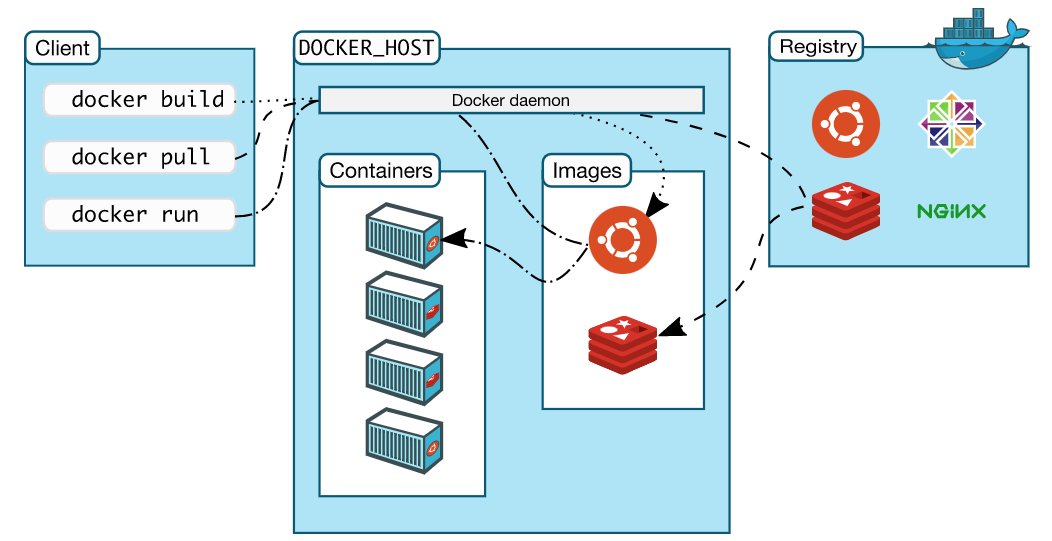
\includegraphics[width=1.0\textwidth]{./images/docker_architecture.png}
  \caption{Arhitektura platforme \emph{Docker}}
  \label{fig:dockerarch}
\end{figure}

Koraci potrebni da se napravi slika aplikacije se definišu u datoteci \emph{Dockerfile}. Svaka instrukcija u ovom fajlu kreira po jedan sloj slike (eng. \emph{layer}). U slučaju \emph{.NET Core} aplikacija, prvi korak je učitavanje željenog radnog okvira, zatim, (primera radi) pokretanje prevođenja izvornog koda i smeštanje izvršnog koda na željenu lokaciju. Krajnji korak je uglavnom definisanje komande za pokretanje aplikacije. Bitno je naglasiti da tokom razvijanja aplikacije, \emph{Docker} prepoznaje koji su se slojevi slike promenili, te ponovo kreira samo njih i njihove naredne slojeve. Ovo čini generisanje slike efikasnom i brzom operacijom koja ne usporava programera, koji najčeće menja samo neke delove aplikacije. Kreirane slike se čuvaju u registru slika koji može biti lokalni ili negde u oblaku.

Kontejner sadrži specifikaciju operativnog sistema na kojem se pokreće slika, i on može biti \emph{Windows}, \emph{Mac} i \emph{Linux}. Kontejneri koji odgovaraju drugom operativnom sistemu se pokreću u odgovarajućoj virtuelnoj mašini.

Korišćeno okruženje za lokalno kreiranje i pokretanje kontejnera je \emph{Docker Desktop} \cite{DockerDesktop} prikazan na slici \ref{fig:dockerdesktop}. \emph{Docker Desktop} u sebi sadrži virtuelnu mašinu \emph{Linux} u okviru koje se pokreću kontejneri \emph{Linux}.

\begin{figure}[!ht]
  \centering
  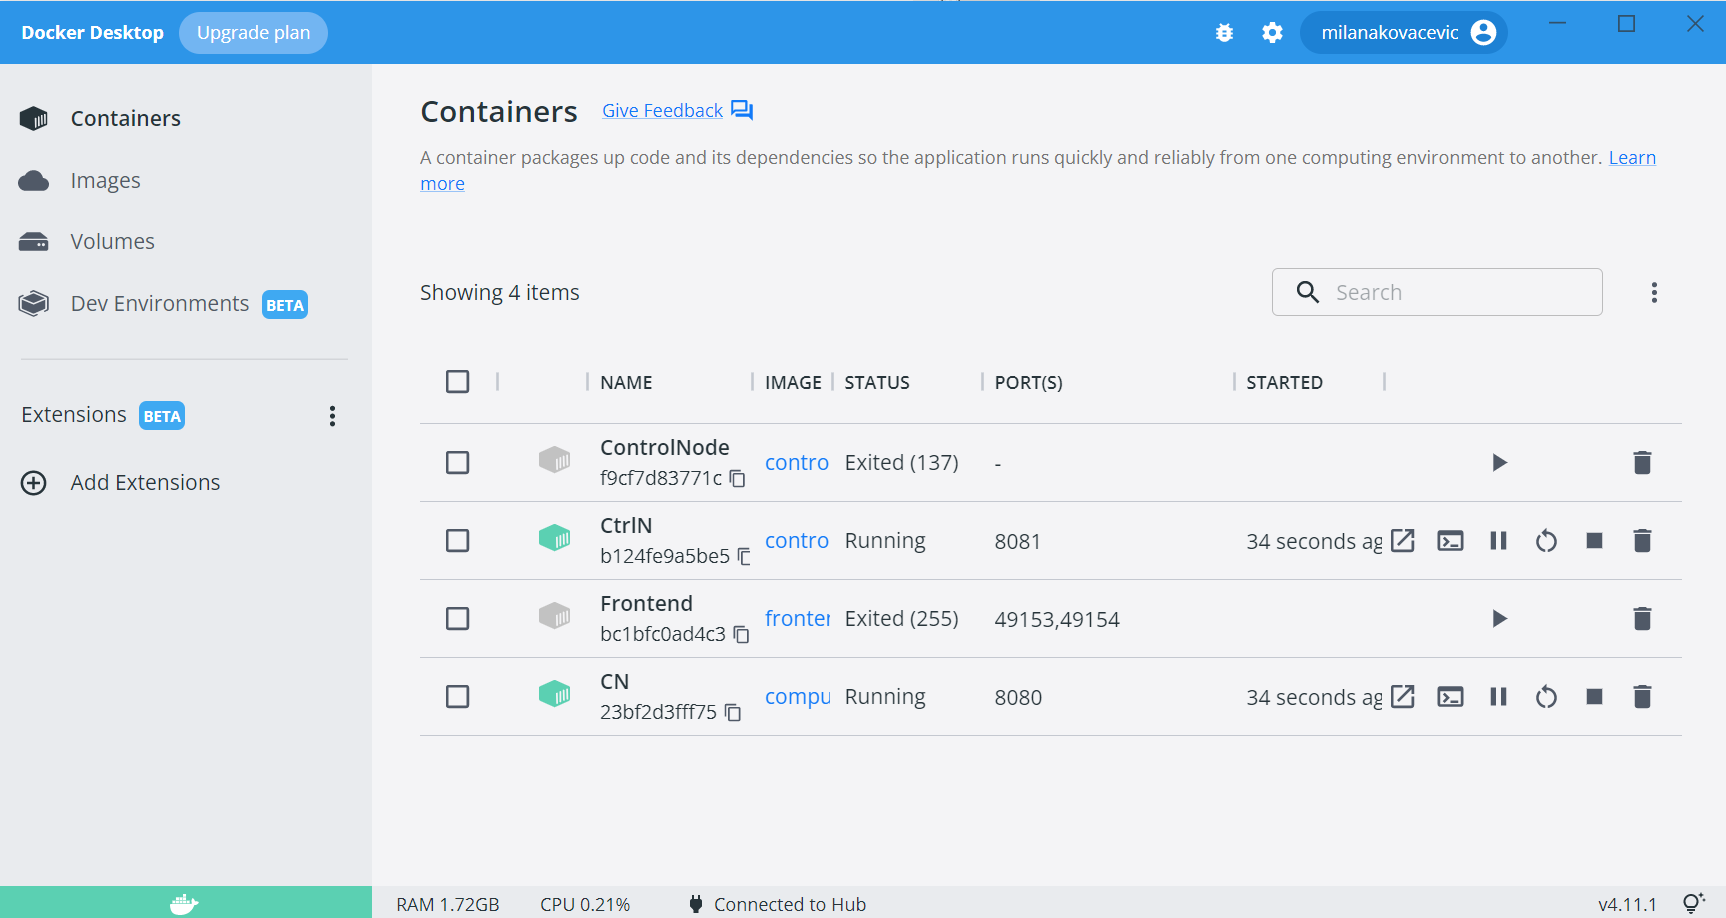
\includegraphics[width=1.0\textwidth]{./images/docker_desktop.png}
  \caption{Docker Desktop}
  \label{fig:dockerdesktop}
\end{figure}

% Kubernetes detalji
\subsection{Platforma Kubernetes}
\label{subs:kubernetes_platform}

Pokretanje sistema na praktičan i skalabilan način, omogućila je platforma \emph{Kubernetes} \cite{Kubernetes}. Ona pruža potrebnu infrastrukturu za pokretanje aplikacija zapakovanih u \emph{Docker} kontejnere, kao i za upravljanje njima i ostalim pratećim delovima sistema.

Kubenetes omogućava:
\begin{enumerate}
\item Pronalaženje servisa koristeći \emph{DNS} ime ili \emph{IP} adresu,
\item Balansiranje saobraćaja kroz mrežu u zavisnosti od opterećenosti,
\item Korišćenje diska i drugih skladišta podataka,
\item Automatsko ažuriranje (eng. \emph{update}) verzija aplikacije kao i vraćanje na prethodnu verziju,
\item Upravljanje resursima i pakovanje kontejnera na mašine,
\item \emph{Self-healing} - automatski restart kontejnera koji ne ispunjavaju uslove zdravlja,
\item Upravljanje konfiguracijom, šiframa, sertifikatima i drugim osetljivim informacijama - uz samostalno ažuriranje bez potrebe za promenom slike kontejnera.
\end{enumerate}

Na slici \ref{fig:kubernetesarh} prikazana je arhitektura klastera Kubernetes, preuzeta iz zvanične dokumentacije \cite{KubernetesArchitecture}.

\begin{figure}[!ht]
  \centering
  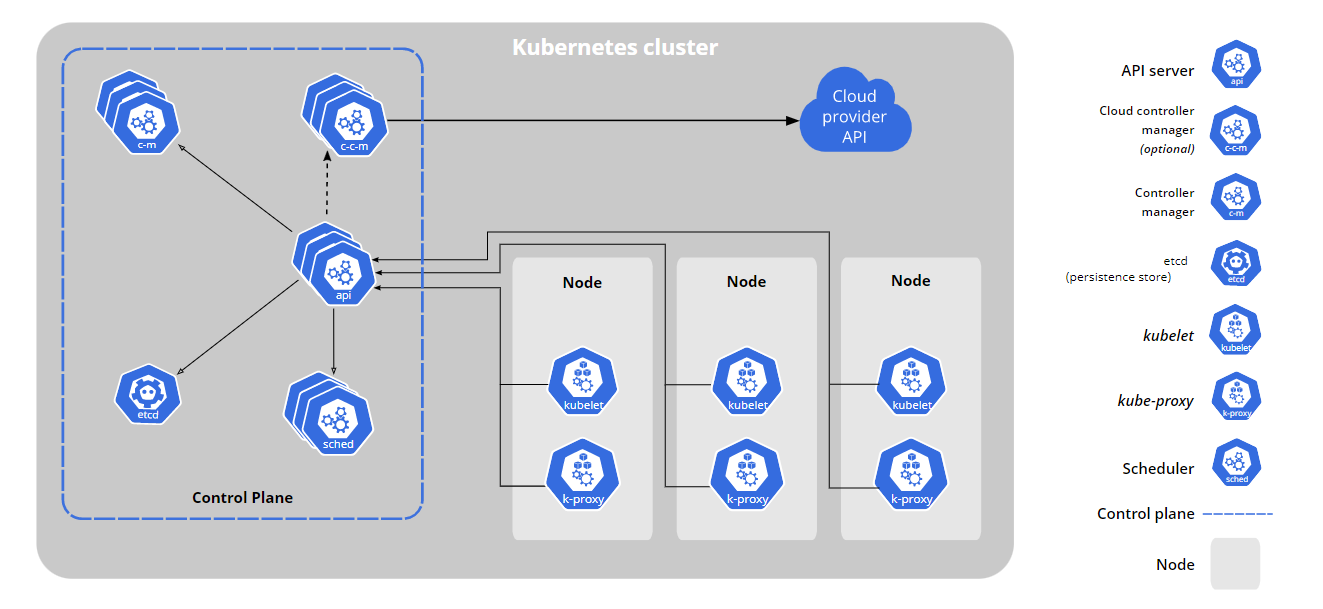
\includegraphics[width=1.0\textwidth]{./images/kubernetes_architecture.png}
  \caption{Arhitektura klastera Kubernetes}
  \label{fig:kubernetesarh}
\end{figure}

Klaster Kubernetes se sastoji iz dve celine: kontrolnog dela i skupa radnih mašina (eng. \emph{nodes}). Radne mašine na sebi pokreću \emph{mahune} (eng. \emph{pod}) u okviru kojih je smešten jedan ili više kontejnera, a u okviru svakog se nalazi aplikacija. Mahuna je najmanja jedinica koju je moguće kreirati i pokrenuti na klasteru, a kontejneri unutar njega imaju istu specifikaciju i dele lokalnu mrežu.

Kako bi pokrenute aplikacije bile dostupne na mreži, kreira se apstrakcija koja se naziva \emph{Servis}. Ova apstrakcija povezuje grupu mahuna i definiše način na koji im se pristupa: koristeći jedinstveno \emph{DNS} ime ili \emph{IP} adresu (eng. \emph{Service endpoints}). Slanjem poruka na ovu adresu, Kubernetes sam usmerava i balansira saobraćaj ka mahunama, od kojih svaka ima jedinstvenu \emph{IP} adresu.

U okviru svake radne mašine je pokrenuto još nekoliko sistemskih procesa: 
\begin{enumerate}
\item \emph{kuberlet} - Zadužen za pokretanje kontejnera na mašini, kao i za praćenje rada kontejnera i njihovog zdravlja.
\item \emph{kube-proxy} - Zadužen za podešavanje pravila mreže koja omogućavaju slanje i prijem poruka mahunama, koristeći specifikacije definisane servisima.
\item \emph{Container runtime} - Zadužen za pokretanje kontejnera.
\end{enumerate}

Kontrolni deo klastera služi za upravljanje klasterom, a funkcionalnosti su obezbeđene kroz nekoliko komponenti:
\begin{enumerate}
\item \emph{kube-apiserver} - Server API koji prima zahteve upućene klasteru.
\item \emph{etcd} - Služi kao skladište podatka u klasteru.
\item \emph{kube-scheduler} - Zadužen za smeštanje novih mahuna na mašine u skladu sa dostupnim i traženim resursima, kao i drugim specifikacijama (na primer, međusobni afinitet servisa).
\item \emph{kube-controller-manager} - Sastoji se od nekoliko kontrolera:
	\begin{enumerate}
	\item \emph{node-controller} - Omogućava reagovanje u slučajevima kada mašine postanu nedostupne.
	\item \emph{job-controller} - Izvšava dodatne poslove na klasteru.
	\item \emph{endpoints-controller} - Podešava endpointe, tj. omogućava pronalaženje servisa i mahuna koje obuhvata. Ažurira adrese u slučaju promena (dodavanja i brisanja mahuna).
	\item \emph{Service Account \& Token Controller} - Resursi u okviru klastera se mogu podeliti po imenskim prostorima (eng. \emph{namespace}). Ovi kontroleri omogućavaju podešavaju prava pristupa u okviru imenskih prostora.
	\end{enumerate}
\item \emph{cloud-controller-manager} - Predstavlja vezu između klastera i snabdevača resursa u oblaku (eng.\emph{cloud provider}).
\end{enumerate}
Sve aplikacije su pokrenute na fizičkim (ili virtuelnim) mašinama koje su date na raspolaganju klasteru tokom njegovog kreiranja ili ažuriranja. Neki kontejneri/mahune mogu biti pokrenuti na istoj mašini, ali to zavisi od potražnje i raspodele resursa, kao i od drugih specifikacija. Jedna od prednosti Kubernetesa je što on vodi računa o tome gde je koji proces pokrenut, te pokušava da obezbedi najbolju otpornost na greške u sistemu (na primer, restartovanje mašine) i time obezbedi visoku dostupnost pokrenutih servisa.

Dodatno, visoka dostupnost servisa se obezbeđuje kroz kontrolisani proces ažuriranja aplikacija, koristeći mehanizam koji se naziva eng. \emph{rolling update}. Ovaj sistem podrazumeva da se inkrementalno zamenjuju mahune, sa novokreiranim mahunama koje su pokrenute sa novom verzijom. Tokom ažuriranja, saobraćaj do mahuna se automatski raspoređuje samo ka dostupnim mahunama.

Za definisanje resursa i njihovih specifikacija, kao i konfiguracije na klasteru koriste se datoteke u formatu \emph{yaml}. Prosleđivanjem ovih datoteka klasteru se rade promene na klasteru.

Za komunikaciju sa kontrolnim delom Kubernetes klastera se koristi kilijent \emph{kubectl}. Neke od komandi su predstavljene u nastavku.

\begin{verbatim}
// Opšti oblik komande
kubectl [command] [TYPE] [NAME] [flags]
// Pravljenje resursa i njihovih specifikacija
kubectl apply -f deploy.yaml
// Izlistavanje servisa na klasteru
kubectl get svc
// Izlistavanje mahuna
kubectl get pods
// Pristup bash konzoli na mašini u okviru koje je pokrenuta mahuna
kubectl exec mypod-m96mk -it mypod-m96mk  -- /bin/bash
// Podešava automatsko skaliranje broja mahuna
kubectl autoscale deployment computenode --cpu-percent=50 --min=1 --max=10
\end{verbatim}

\subsection{Platforma \emph{Microsoft Azure}}
\label{sub:azureplatform}

Programska implementacija sistema je uključila njegovo pokretanje u oblaku, a za to je korišćena platforma \emph{Microsoft Azure} \cite{Azure}. Ova platforma pruža veliki broj softverskih i infrastrukturnih rešenja, kao i propratnih servisa i mogućnosti koje poboljšavaju celokupno iskustvo korišćenja.

Najrelevantniji resursi korišćeni za pokretanje sistema u na \emph{Azure} platformi su:
\begin{enumerate}
\item \emph{Azure Kubernetes Service} (skr. AKS) \cite{AKS} - Resurs koji predstavlja klaster \emph{Kubernetes}.
\item \emph{Azure SQL Database} (skr. AzureSQLDB) \cite{AzureSQLDB} - Resurs koji predstavlja relacionu bazu podataka.
\item \emph{Azure Active Directory} \cite{AAD} (skr. AAD) - Resurs koji omogućava kreiranje identiteta (npr. korisnike, grupe) i njihovo podešavanje (prava pristupa, login...).
\item \emph{Azure Monitor} (skr. AM) \cite{AzureMonitor} - Skup propratnih funkcionalnosti koje pružaju uvid u ponašanje Azure resursa. Sakuplja logove i metrike, daje alate za njihovo analiziranje, kao i mogućnost uzbunjivanja (eng. \emph{alerts}) i reagovanja na dešavanja od interesa. Ima podršku i za tehnike mašinskog učenja nad sakupljenim podacima. Opis integracije sa servisom \emph{Azure Monitor} se nalazi u odeljku \ref{chp:pracenjemetrika} - Praćenje rada sistema.
\end{enumerate}

\subsection{Dodatni alati}
\label{sub:dodatnialati}

\subsubsection{Swagger / OpenAPI}

\emph{OpenAPI} \cite{OpenAPI} je specifikacija \emph{REST API}-a (eng. \emph{Application Programming Interface}) koja ne zavisi od programskog jezika. \emph{Swagger} \cite{Swagger} predstavlja skup alata koji koriste \emph{OpenAPI} specifikaciju.

Korišćenjem skupa alata \emph{Swagger}, moguće je dokumentovati serverski \emph{web REST API} na standardizovan način, u datoteci formata \emph{json}. Za pravljenje ove specifikacije, koristi se alat \emph{Swashbuckle} \cite{Swashbuckle}.

Za generisanje klijenta u radnom okviru \emph{.NET Core}, koristi se alat \emph{NSwag} \cite{NSwag}. Na osnovu prethodno generisane datoteke \emph{json}, on generiše klasu koja sadriži \emph{HTTP} klijenta i potrebnu dokumentaciju. Ovo je praktičan i efikasan način da se automatski generiše kod klijenta pomoću kojeg se šalju zahtevi serveru.

Opis korišćenja skupa alata \emph{Swagger} se nalazi u odeljcima \ref{sec:implementacija} - Implementacija i \ref{sec:testiranjesistema} - Okvir za testiranje.


% ------------------------------------------------------------------------------
\chapter{Sistem DCS}
\label{chp:sistemdcs}
% ------------------------------------------------------------------------------

Kao sastavni deo master rada razvijen je projekat nazvan \emph{Distributed Computation System} (skr. \emph{DCS}).

Glavni zadatak sistema je da omogući korisniku obradu podataka na distribuirani način.
U jednostavnom slučaju, sistem obrađuje prosleđeni niz atomičnih poslova, a zatim agregira njihove rezultate. Ovo predstavlja distribuiranu implementaciju funkcionalnosti eng. \emph{map-reduce}.
U naprednijem slučaju, sistem DCS je moguće usko specijalizovati za obradu određenog tipa posla. Tada se prilikom implementacije koristi i poznavanje prirode posla, što omogućava da se on podeli na podjedinice. Krajnji rezultat se takodje dobija agregiranjem podrezultata, s tim da podjedinice posla mogu biti međusobno zavisne, te je za celokupno izvršavanje posla potrebno pratiti plan distribuiranog izvršavanja.

% TODO primer nekog kompleksnijeg posla

Jedan od glavnih ciljeva sistema DCS je njegova modularnost i primenljivost. Njega je, uz jednostavne izmene, moguće proširiti kako bi podržao različite tipove poslova koje su od značaja njegovim korisnicima, oslanjajući se pritom na zajedničku infrastrukturu za obradu poslova. Ova infrastruktura je opisana u narednim poglavljima.

%, a predstavlja glavni deo sistema koji služi za zakazivanje i praćenje poslova, kao i čuvanje rezultata izvršavanja.

% ------------------------------------------------------------------------------
\section{Funkcionalnosti}
\label{chp:opisfunkc}
% ------------------------------------------------------------------------------

%Pre opisivanja slucajeva upotrebe bi trebalo da se oni ukratko navedu, sa nazivima i kratkim opisima
%	- lakse je razumeti pojedinacan slucaj ako se razume kontekst u kome se on nalazi
%	- mozda ima smisla staviti i neki dijagram aktivnosti ili bolje BPMN koji povezuje slucajeve upotrebe, tj. njihove ulaze i izlaze

U ovom poglavlju je prikazan pregled funkcionalnosti sistema za distribuirano izračunavanje DCS. 
Glavna funkcionalnost sistema je obrada korisnikovih zahteva za izvršavanje poslova. 

U nastavku se nalaze BPMN dijagrami (eng. \emph{Business Process Modeling Notation}) koji opisuju saradnju između korisnika i sistema. Na slici \ref{fig:bpmn_korisnik} je predstavljen tok saradnje koji uključuje pravljenje posla i njegovo izvršavanje.  Na slici \ref{fig:bpmn_korisnik_rez} je predstavljena saradnja prilikom preuzimanja rezultata, a na slici \ref{fig:bpmn_otkazivanje} je opisana saradnja prilikom otkazivanja prethodno napravljenog posla.

\begin{figure}[!ht]
  \centering
  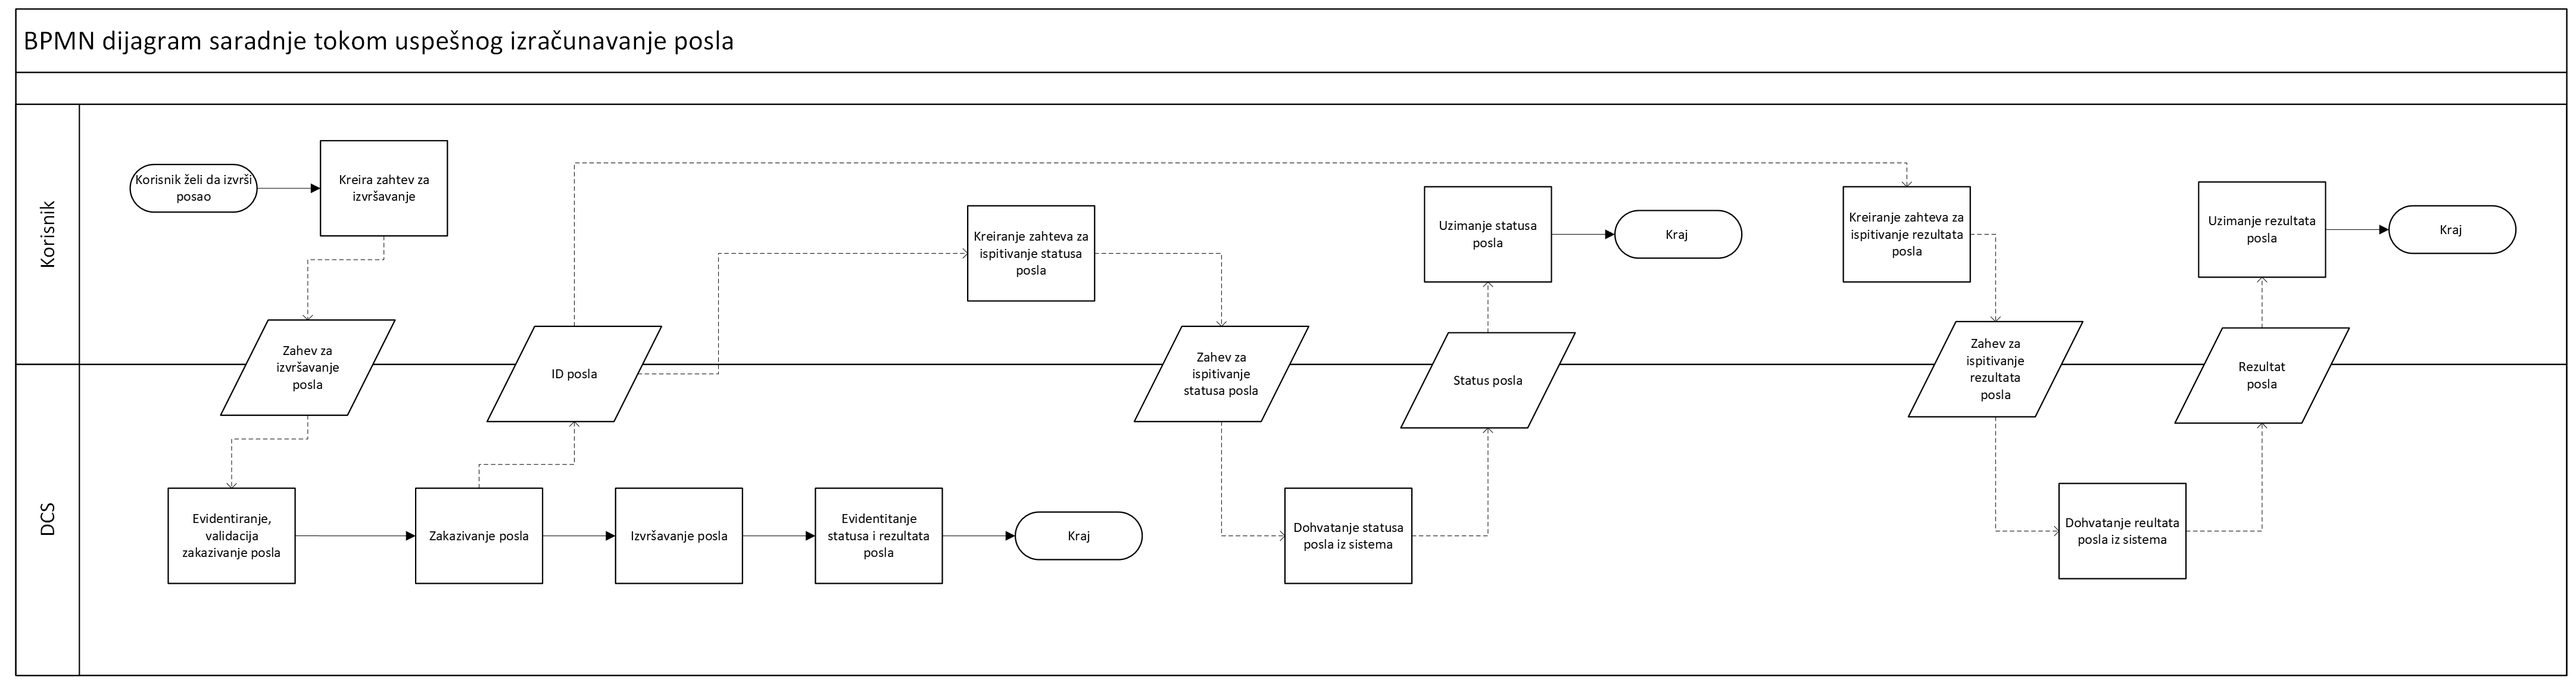
\includegraphics[width=1\textwidth]{./images/BPMN_dijagram_saradnje_korisnik_dsc.png}
  \caption{BMPN dijagram saradnje - Pravljenje zahteva za izvršavanje i provera statusa posla}
  \label{fig:bpmn_korisnik}
\end{figure}

\begin{figure}[!ht]
  \centering
  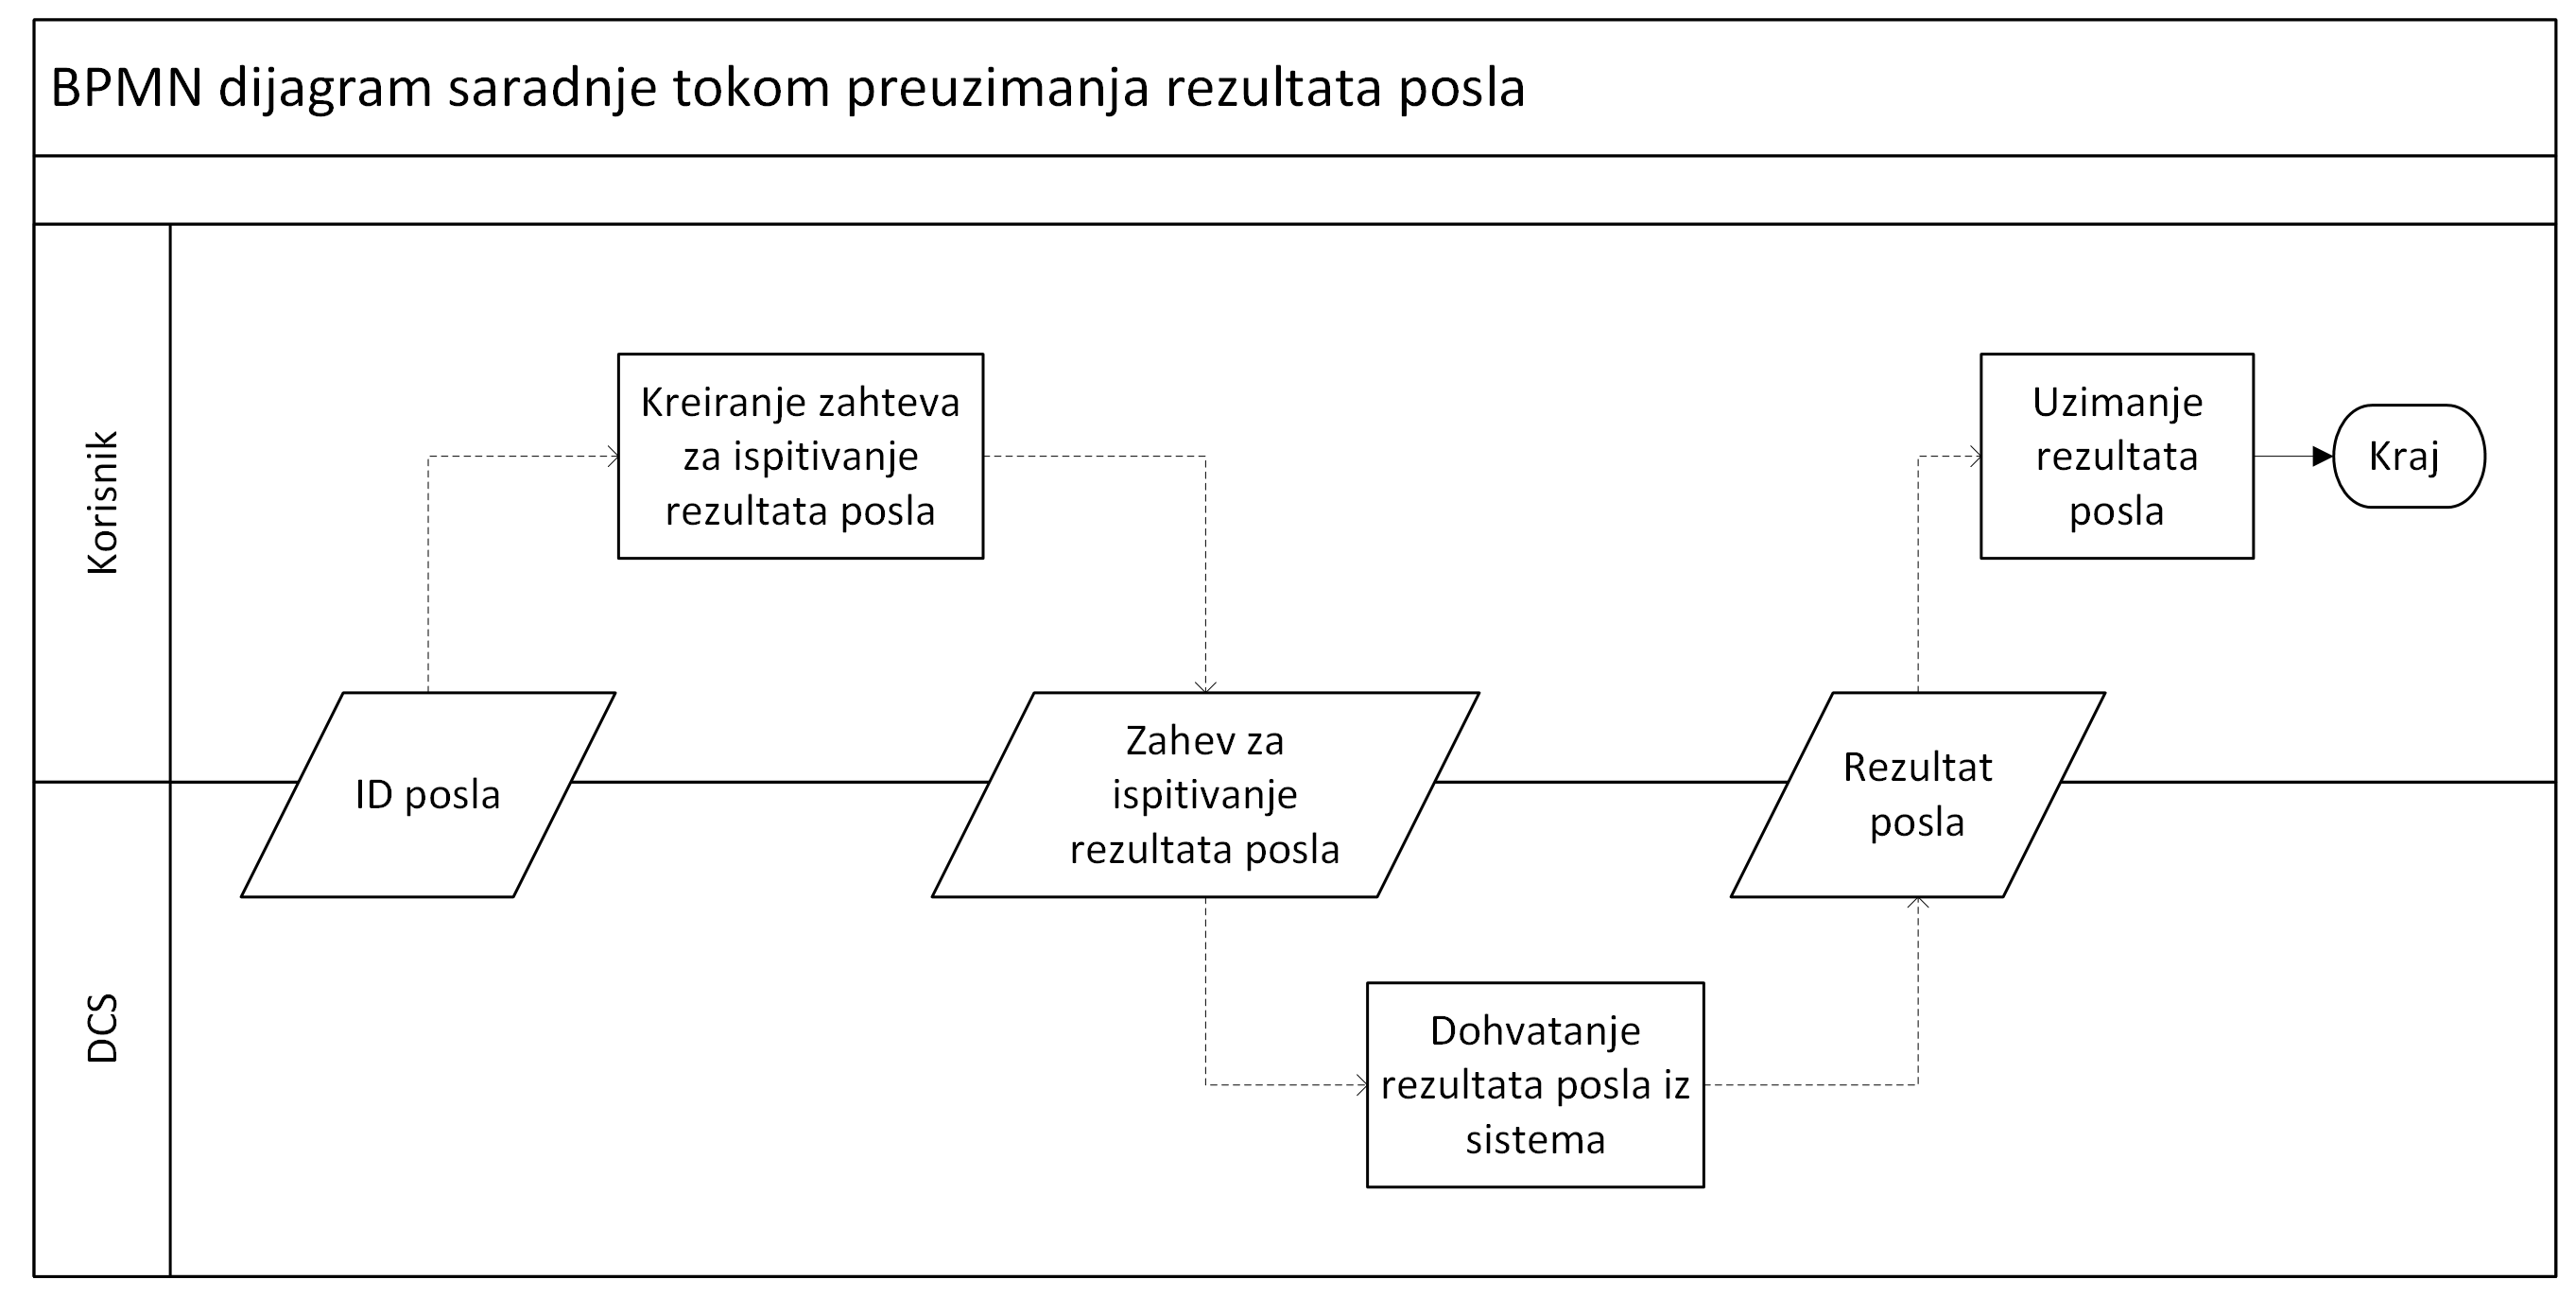
\includegraphics[width=1\textwidth]{./images/BPMN_dijagram_saradnje_korisnik_dsc_rezultati.png}
  \caption{BMPN dijagram saradnje - Preuzimanje rezultata}
  \label{fig:bpmn_korisnik_rez}
\end{figure}

\begin{figure}[!ht]
  \centering
  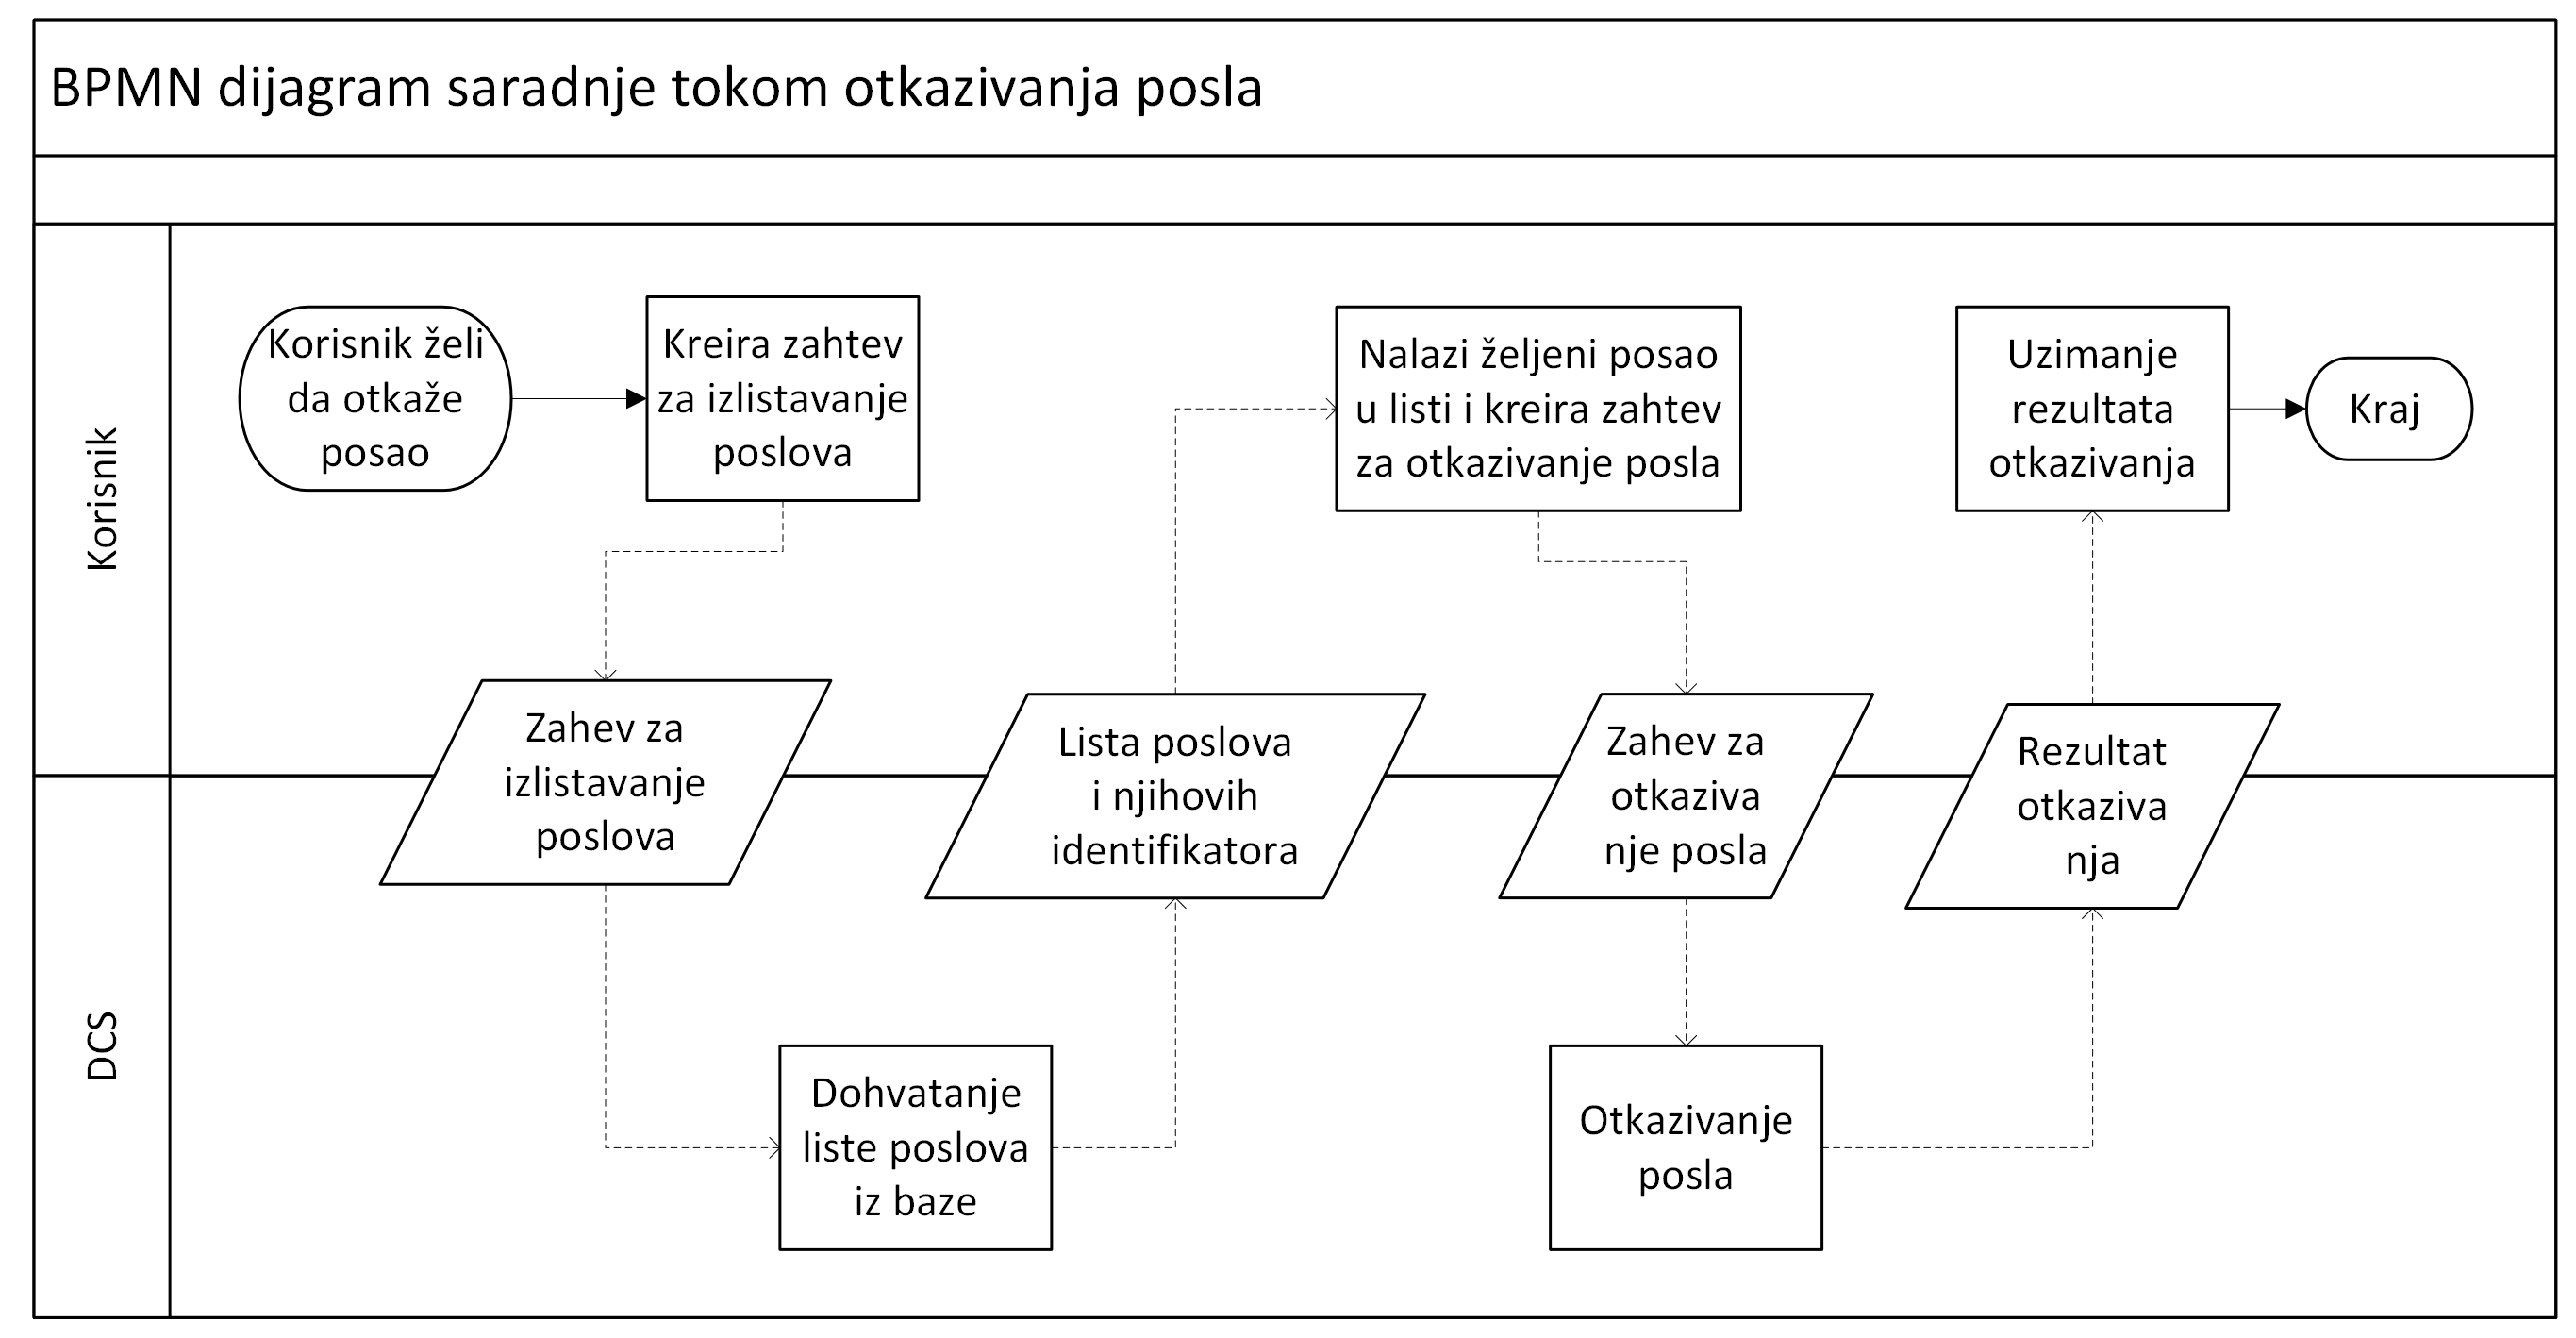
\includegraphics[width=1\textwidth]{./images/BPMN_dijagram_saradnje_otkazivanje.png}
  \caption{BMPN dijagram saradnje - Otkazivanje posla}
  \label{fig:bpmn_otkazivanje}
\end{figure}

U narednim odeljcima su opisane funkcionalnosti kroz slučajeve upotrebe, iz ugla korisnika i iz ugla dva tipa administratora: bezbednosnog i klaster administratora.

\subsection{Slučajevi upotrebe - Korisnik}

Slučajevi upotrebe iz ugla korisnika su:
\begin{enumerate}
\item Pravljenje posla - Prvi korak koji korisnik radi kako bi zaposlio sistem DCS da izvršava posao.
\item Pregled poslova - Izlistavanje jednog ili više poslova kako bi korisnik preuzeo status o uspešnosti, kao i identifikatore poslova.
\item Preuzimanje rezultata izvršavanja posla - Kada je posao izvršen, korisnik preuzima rezultate.
\item Otkazivanje posla - Korisnik ima mogućnost da prekine izvršavanje prethodno napravljenog posla.
\end{enumerate}

Ovi slučajevi upotrebe su prikazani na slici \ref{fig:slucajupotrebe_korisnik}, a detaljnije su opisani u narednim odeljcima.

\begin{figure}[!ht]
  \centering
  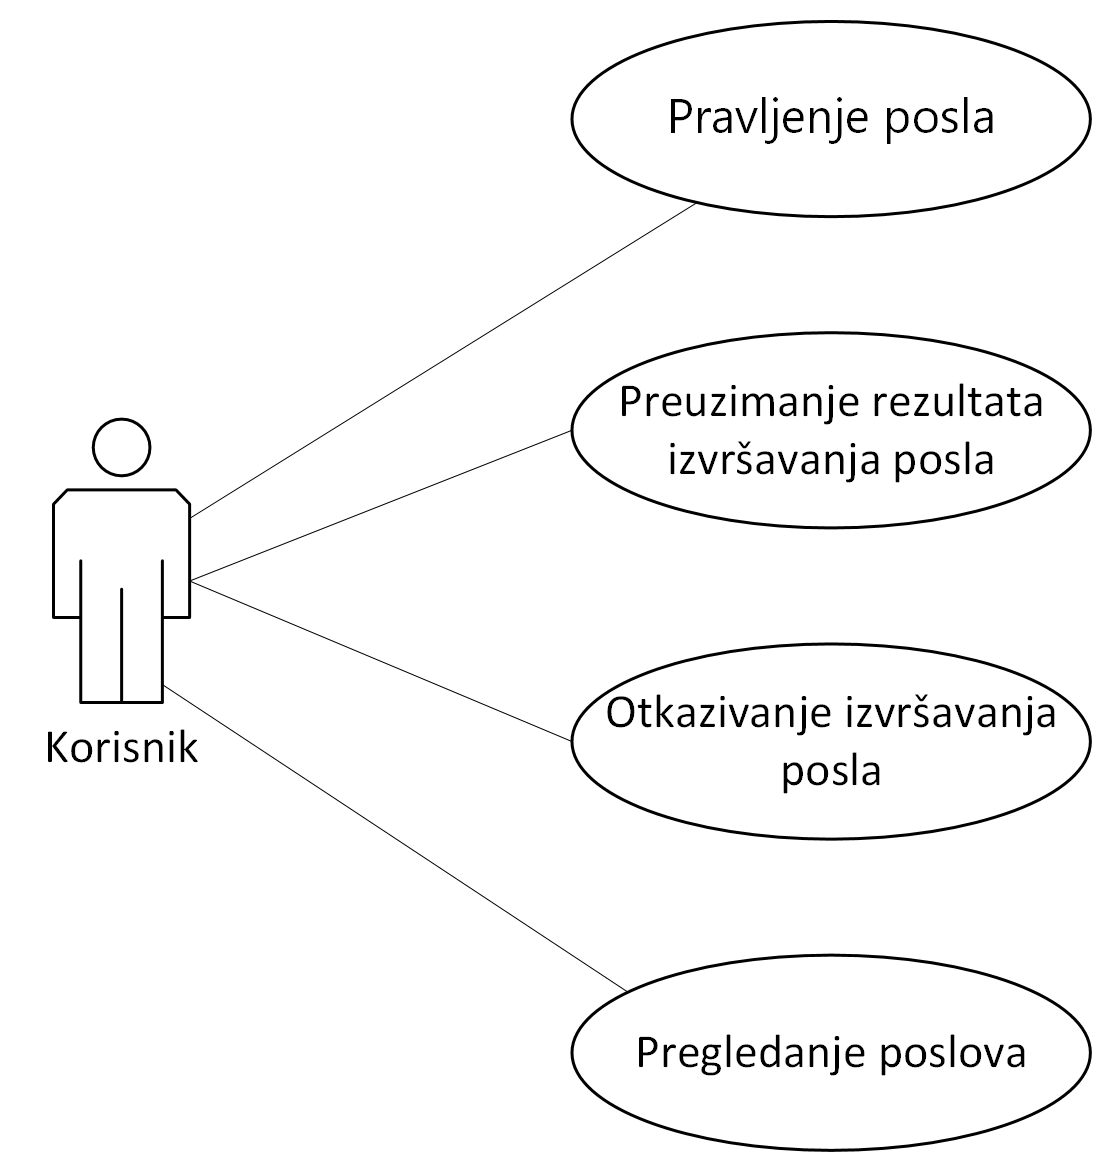
\includegraphics[width=0.6\textwidth]{./images/dijagram_slucajeva_upotrebe_korisnik.png}
  \caption{UML dijagram slučajeva upotrebe - Korisnik}
  \label{fig:slucajupotrebe_korisnik}
\end{figure}

% Kreiranje posla
\subsubsection{Pravljenje posla}

\begin{enumerate}
\item Naziv: Pravljenje posla.
\item Akter: Korisnik koji želi da izvrši posao nad ulaznim podacima.
\item Kratak opis: Korisnik šalje zahtev za kreiranje posla. Sistem validira zahtev i vraća potvrdu o uspešnosti primanja zahteva.
\item Preduslovi: Korisnik ima pristup internetu. Korisnik ima neophodna prava da bi poslao zahtev sistemu. Sistem je u funkciji.
\item Postuslovi: Sistem je evidentirao novi zahtev za posao i prosledio ga na asinhrono izvršavanje.
\item Tok događaja:
	\begin{enumerate}
	\item \label{zak:pravizahtev}Korisnik pravi zahtev za dodavanje posla. Zahtev se sastoji od:
		\begin{enumerate}
		\item Specifikacije tipa posla,
		\item Niza ulaznih podataka.
		\end{enumerate}
	\item \label{zak:saljezahtev} Korisnik šalje zahtev sistemu preko interneta koristeći definisani interfejs.
	\item \label{zak:proveraprava} Sistem proverava prava korisnika.
	\item \label{zak:validacijazahteva} Sistem validira novopridošli zahtev za izvršavanje posla.
	\item Sistem evidentira novi zahtev za izvršavanje u bazi.
	\item \label{zak:asinhzakazivanje} Sistem stavlja zahtev u red za asinhrono izvršavanje.
	\item Korisnik dobija potvrdu da je posao prihvaćen i identifikator po kojem je posao zaveden u sistemu.
	\end{enumerate}
\item Alternativni tok događaja:
	\begin{enumerate}
	\item Korisnik nema prava da podnese zahtev. Ukoliko u koraku \ref{zak:proveraprava} korisnik nema neophodna prava, sistem odbija zahtev uz odgovarajuću grešku. Proces se nastavlja u koraku \ref{zak:saljezahtev} glavnog toka.
	\item Zahtev je neispravan. Ukoliko u koraku \ref{zak:validacijazahteva} sistem prepozna neispravan zahtev, odbija ga uz odgovarajuću grešku. Neispravan zahtev može biti:
		\begin{enumerate}
		\item Neispravna specifikacija tipa posla. Zahtevani tip posla mora biti podržan od strane sistema,
		\item Format ulaznih podataka nije odgovarajući.
		\end{enumerate}
Proces se nastavlja u koraku \ref{zak:pravizahtev} glavnog toka.
	\item Sistem je preopterećen i nema dovoljno resursa da zakaže novi posao. Ukoliko u koraku \ref{zak:asinhzakazivanje} sistem proceni da nema dovoljno resursa za izvršavanje posla, on odbija zahtev uz grešku da je sistem preopterećen i da korisnik pokuša kasnije. Proces se nastavlja u koraku \ref{zak:saljezahtev} glavnog toka.
	\end{enumerate}
\item Podtokovi: /
\item Specijalni zahtevi: /
\item Dodatne informacije: /
\end{enumerate}

% Pregled poslova
\subsubsection{Pregled poslova}
\begin{enumerate}
\item Naziv: Pregled poslova.
\item Akter: Korisnik koji želi da preuzme listu evidentiranih poslova u sistemu.
\item Kratak opis: Korisnik šalje zahtev za izlistavanje evidentiranih poslova. Sistem validira zahtev i vraća tražene informacije o evidentiranim poslovima.
\item Preduslovi: Korisnik ima pristup internetu. Korisnik ima neophodna prava da bi poslao zahtev sistemu. Sistem je u funkciji. Posao je izvršen i rezultati su dostupni u bazi.
\item Postuslovi: Sistem je prosledio rezultate izvršavanja korisniku.
\item Tok događaja:
	\begin{enumerate}
	\item \label{pregledp:konstruisezahtev} Korisnik pravi zahtev za izlistavanje poslova.
	\item \label{pregledp:saljezahtev} Korisnik šalje zahtev sistemu preko interneta koristeći definisani interfejs.
	\item \label{pregledp:proveraprava} Sistem proverava prava korisnika.
	\item \label{pregledp:slanjeliste} Sistem šalje listu evidentiranih poslova dostupnih u bazi.
	\item Korisnik dobija listu evidentiranih poslova.
	\end{enumerate}
\item Alternativni tok događaja:
	\begin{enumerate}
	\item Korisnik nema prava da podnese zahtev. Ukoliko u koraku \ref{pregledp:proveraprava} korisnik nema neophodna prava, sistem odbija zahtev uz odgovarajuću grešku. Proces se nastavlja u koraku \ref{pregledp:saljezahtev} glavnog toka.
	\end{enumerate}
\item Podtokovi: /
\item Specijalni zahtevi: /
\item Dodatne informacije: Rezultujuća lista poslova sadrži informacije o svakom evidentiranom poslu, i to:
	\begin{enumerate}
	\item Identifikator posla,
	\item Status posla,
	\item Vreme početka izvršavanja posla,
	\item Vreme završetka izvršavanja posla (ako je posao završen).
	\end{enumerate}
\end{enumerate}

% Dohvatanje rezultata
\subsubsection{Preuzimanje rezultata posla}
\begin{enumerate}
\item Naziv: Preuzimanje rezultata posla.
\item Akter: Korisnik koji želi da pruzme rezultate prethodno zakazanog posla.
\item Kratak opis: Korisnik šalje zahtev za preuzimanje rezultata izvršavanja. Sistem validira zahtev i vraća tražene rezultate.
\item Preduslovi: Korisnik ima pristup internetu. Korisnik ima neophodna prava da bi poslao zahtev sistemu. Sistem je u funkciji. Posao je izvršen i rezultati su dostupni u bazi.
\item Postuslovi: Sistem je prosledio rezultate izvršavanja korisniku.
\item Tok događaja:
	\begin{enumerate}
	\item \label{rez:pravizahtev} Korisnik pravi zahtev za preuzimanje rezultata posla. Zahtev se sastoji od identifikatora posla za koji želi da preuzme rezultate.
	\item \label{rez:saljezahtev} Korisnik šalje zahtev sistemu preko interneta koristeći definisani interfejs.
	\item \label{rez:proveraprava} Sistem proverava prava korisnika.
	\item \label{rez:validacijazahteva} Sistem validira novopridošli zahtev za preuzimanje rezultata posla.
	\item \label{rez:sinhslanjerez} Sistem šalje rezultate korisniku.
	\item Korisnik dobija rezultate.
	\end{enumerate}
\item Alternativni tok događaja:
	\begin{enumerate}
	\item Korisnik nema prava da podnese zahtev. Ukoliko u koraku \ref{rez:proveraprava} korisnik nema neophodna prava, sistem odbija zahtev uz odgovarajuću grešku. Proces se nastavlja u koraku \ref{rez:saljezahtev} glavnog toka.
	\item Zahtev je neispravan. Ukoliko u koraku \ref{rez:validacijazahteva} sistem prepozna da posao sa datim identifikatorom ne postoji, odbija zahtev uz odgovarajuću grešku. Proces se nastavlja u koraku \ref{rez:pravizahtev} glavnog toka.
	\end{enumerate}
\item Podtokovi: /
\item Specijalni zahtevi: /
\item Dodatne informacije: Ukoliko je posao uspešno izvršen, rezultat izvršavanja se sastoji od traženog rezultata izračunavanja. Ukoliko je posao neuspešno obrađen, rezultat se sastoji od informacije o grešci.
\end{enumerate}

% Otkazivanje
\subsubsection{Otkazivanje posla}
\begin{enumerate}
\item Naziv: Otkazivanje posla.
\item Akter: Korisnik koji želi da otkaže prethodno zakazani posao.
\item Kratak opis: Korisnik šalje zahtev za otkazivanje posla. Sistem validira zahtev i vraća potvrdu o uspešnosti otkazivanja.
\item Preduslovi: Korisnik ima pristup internetu. Korisnik ima neophodna prava da bi poslao zahtev sistemu. Sistem je u funkciji.
\item Postuslovi: Sistem je otkazao posao i ažurirao evidenciju posla u bazi.
\item Tok događaja:
	\begin{enumerate}
	\item \label{otk:pravizahtev} Korisnik pravi zahtev za otkazivanje posla. Zahtev se sastoji od identifikatora posla koji želi da otkaže.
	\item \label{otk:saljezahtev} Korisnik šalje zahtev sistemu preko interneta koristeći definisani interfejs.
	\item \label{otk:proveraprava} Sistem proverava prava korisnika.
	\item \label{otk:validacijazahteva} Sistem validira novopridošli zahtev za otkazivanje posla.
	\item \label{otk:sinhotkazivanje} Sistem sinhrono otkazuje sve operacije povezane sa poslom.
	\item Korisnik dobija potvrdu da je posao otkazan.
	\end{enumerate}
\item Alternativni tok događaja:
	\begin{enumerate}
	\item Korisnik nema prava da podnese zahtev. Ukoliko u koraku \ref{otk:proveraprava} korisnik nema neophodna prava, sistem odbija zahtev uz odgovarajuću grešku. Proces se nastavlja u koraku \ref{otk:saljezahtev} glavnog toka.
	\item Zahtev je neispravan. Ukoliko u koraku \ref{otk:validacijazahteva} sistem prepozna da posao sa datim identifikatorom ne postoji ili nije aktivan, odbija zahtev uz odgovarajuću grešku. Proces se nastavlja u koraku \ref{otk:pravizahtev} glavnog toka.
	\end{enumerate}
\item Podtokovi: /
\item Specijalni zahtevi: /
\item Dodatne informacije: /
\end{enumerate}

% Administratorovi slučajevi upotrebe
\subsection{Slučajevi upotrebe - Administrator}

Dodatne funkcionalnosti sistema uključuju slučajeve upotrebe u kojima je učesnik administrator. Ovo uključuje podešavanje bezbednosti i prava pristupa sistemu, kao i prilagođavanje sistema kako bi mogao na što efikasniji način da obradi zahteve korisnika.

Slučajevi upotrebe iz ugla administratora su:
\begin{enumerate}
\item Podešavanja prava pristupa,
\item Podešavanje klastera.
\end{enumerate}

% AAD Admin
\subsubsection{Podešavanja prava pristupa}
Prava pristupa sistemu, tj. delovima sistema dodeljuje administrator za bezbednost. Prava pristupa pojedinačnim delovima sistema se kontrolišu kroz različita prava koja mogu biti dodeljena korisniku. Tipovi prava su:
	\begin{enumerate}
	\item Iskustvo krajnjeg korisnika - Mogućnost slanja zahteva sistemu kroz definisani javni interfejs,
	\item Pravo za praćenje rada sistema - Pristup telemetriji i logovima za praćenje rada sistema,
	\item Administrator klastera - Pristup klasteru za devops akcije,
	\item Administrator bezbednosti.
	\end{enumerate}
Slučajevi upotrebe iz ugla administratora za bezbednost su prikazani na slici \ref{fig:slucajupotrebe_aadadmin}. Ovih slučajevi upotrebe su jednostavni i intuitivni, te nisu opisani u nastavku.

\begin{figure}[!ht]
  \centering
  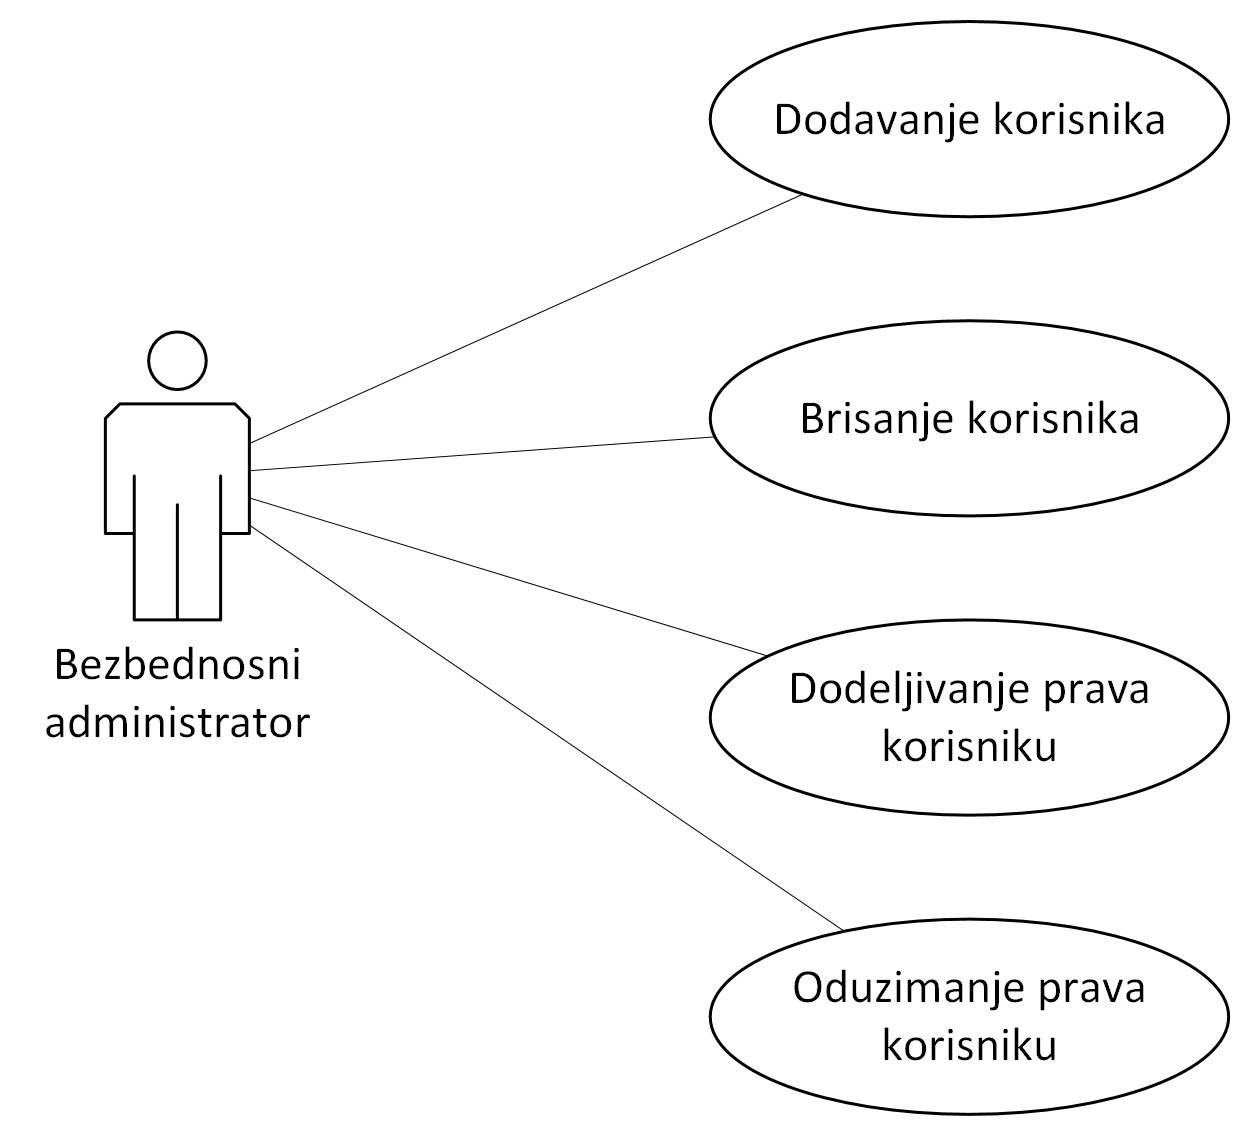
\includegraphics[width=0.6\textwidth]{./images/dijagram_slucajeva_upotrebe_administrator_sistema_aadadmin.png}
  \caption{UML dijagram slučajeva upotrebe - Administrator za bezbednost}
  \label{fig:slucajupotrebe_aadadmin}
\end{figure}


% Podešavanje AKS klastera
\subsubsection{Podešavanje klastera}
Administrator klastera ima mogućnost da menja konfiguraciju sistema kako bi ga prilagodio potrebama krajnjeg korisnika. To uključuje horizontalno i vertikalno skaliranje sistema. Horizontalno skaliranje sistema podrazumeva menjanje broja pokrenutih servisa koji se koriste tokom izvršavanja posla. Vertikalno skaliranje podrazumeva ažuriranje konfiguracije kojom se dodeljuju resursi servisima (dostupna memorija i procesorsko vreme).

Slučajevi upotrebe iz ugla administratora klastera su prikazani na slici \ref{fig:slucajupotrebe_admin_klastera}. Detalji ovih slučajeva upotrebe su konceptualno jasni, a uključuju poznavanje implementacionih detalja, te nisu dalje razrađivani.

\begin{figure}[!ht]
  \centering
  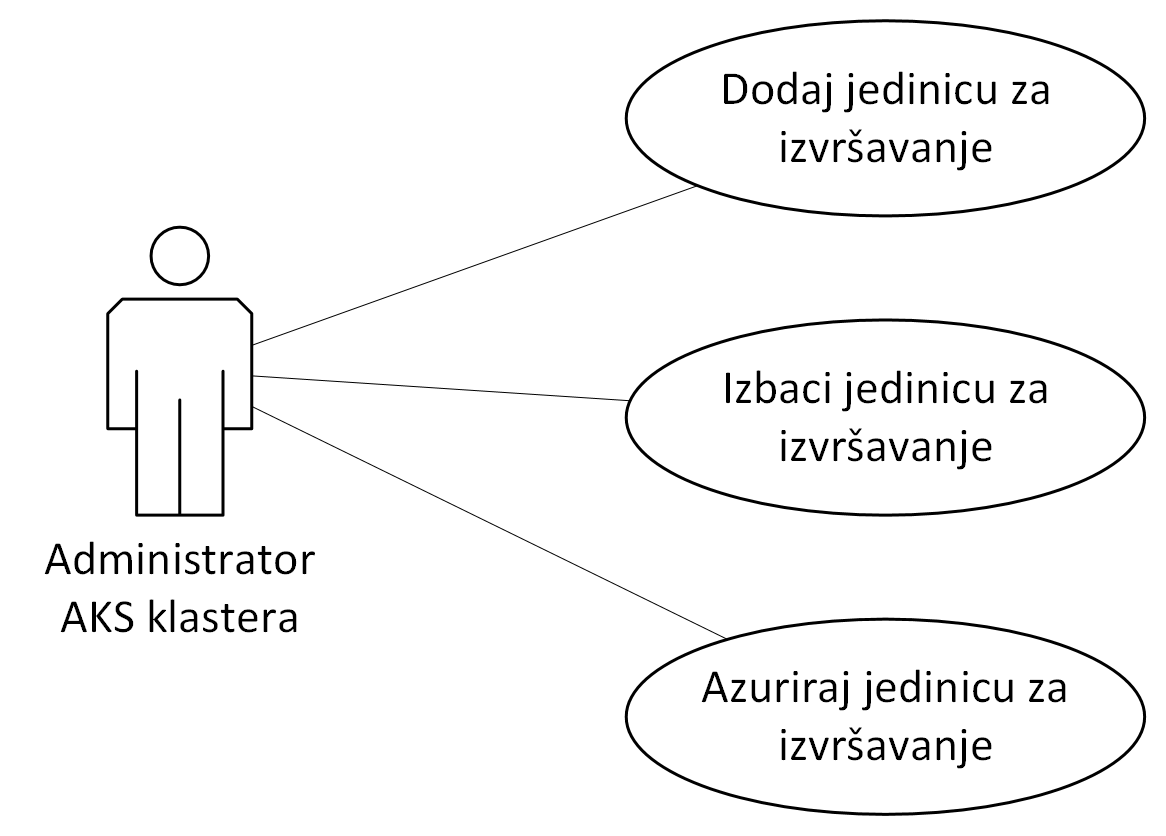
\includegraphics[width=0.6\textwidth]{./images/dijagram_slucajeva_upotrebe_administrator_klastera.png}
  \caption{UML dijagram slučajeva upotrebe - Administrator klastera}
  \label{fig:slucajupotrebe_admin_klastera}
\end{figure}

% ------------------------------------------------------------------------------
\section{Arhitektura sistema}
% ------------------------------------------------------------------------------

Sistem DCS je implementiran po uzoru na arhitekturu klijent-server.

Centralni deo sistema DCS se sastoji od dva tipa aplikacija: Kontrolne jedinice (eng. \emph{Control Node}, skr. CtrlN) i jedinice za izračunavanje (eng. \emph{Compute Node}, skr. CmpN). 
U sistemu postoji tačno jedna aplikacija kontrolne jedinice, koja je zadužena za dve logički odvojene celine: primanje zahteva od korisnika i orkestriranje izvršavanja prethodno zakazanih poslova.
Sa druge strane, u zavisnosti od potreba, DCS se sastoji od jedne ili više jedinica za izračunavanje koje su zadužene za izvršavanje atomičnih (nedeljivih) poslova. CmpN prima zahteve za izvršavanje atomičnih poslova od CtrlN.

Arhitektura sistema je prikazana na slici \ref{fig:arhitektura}.

\begin{figure}[!ht]
  \centering
  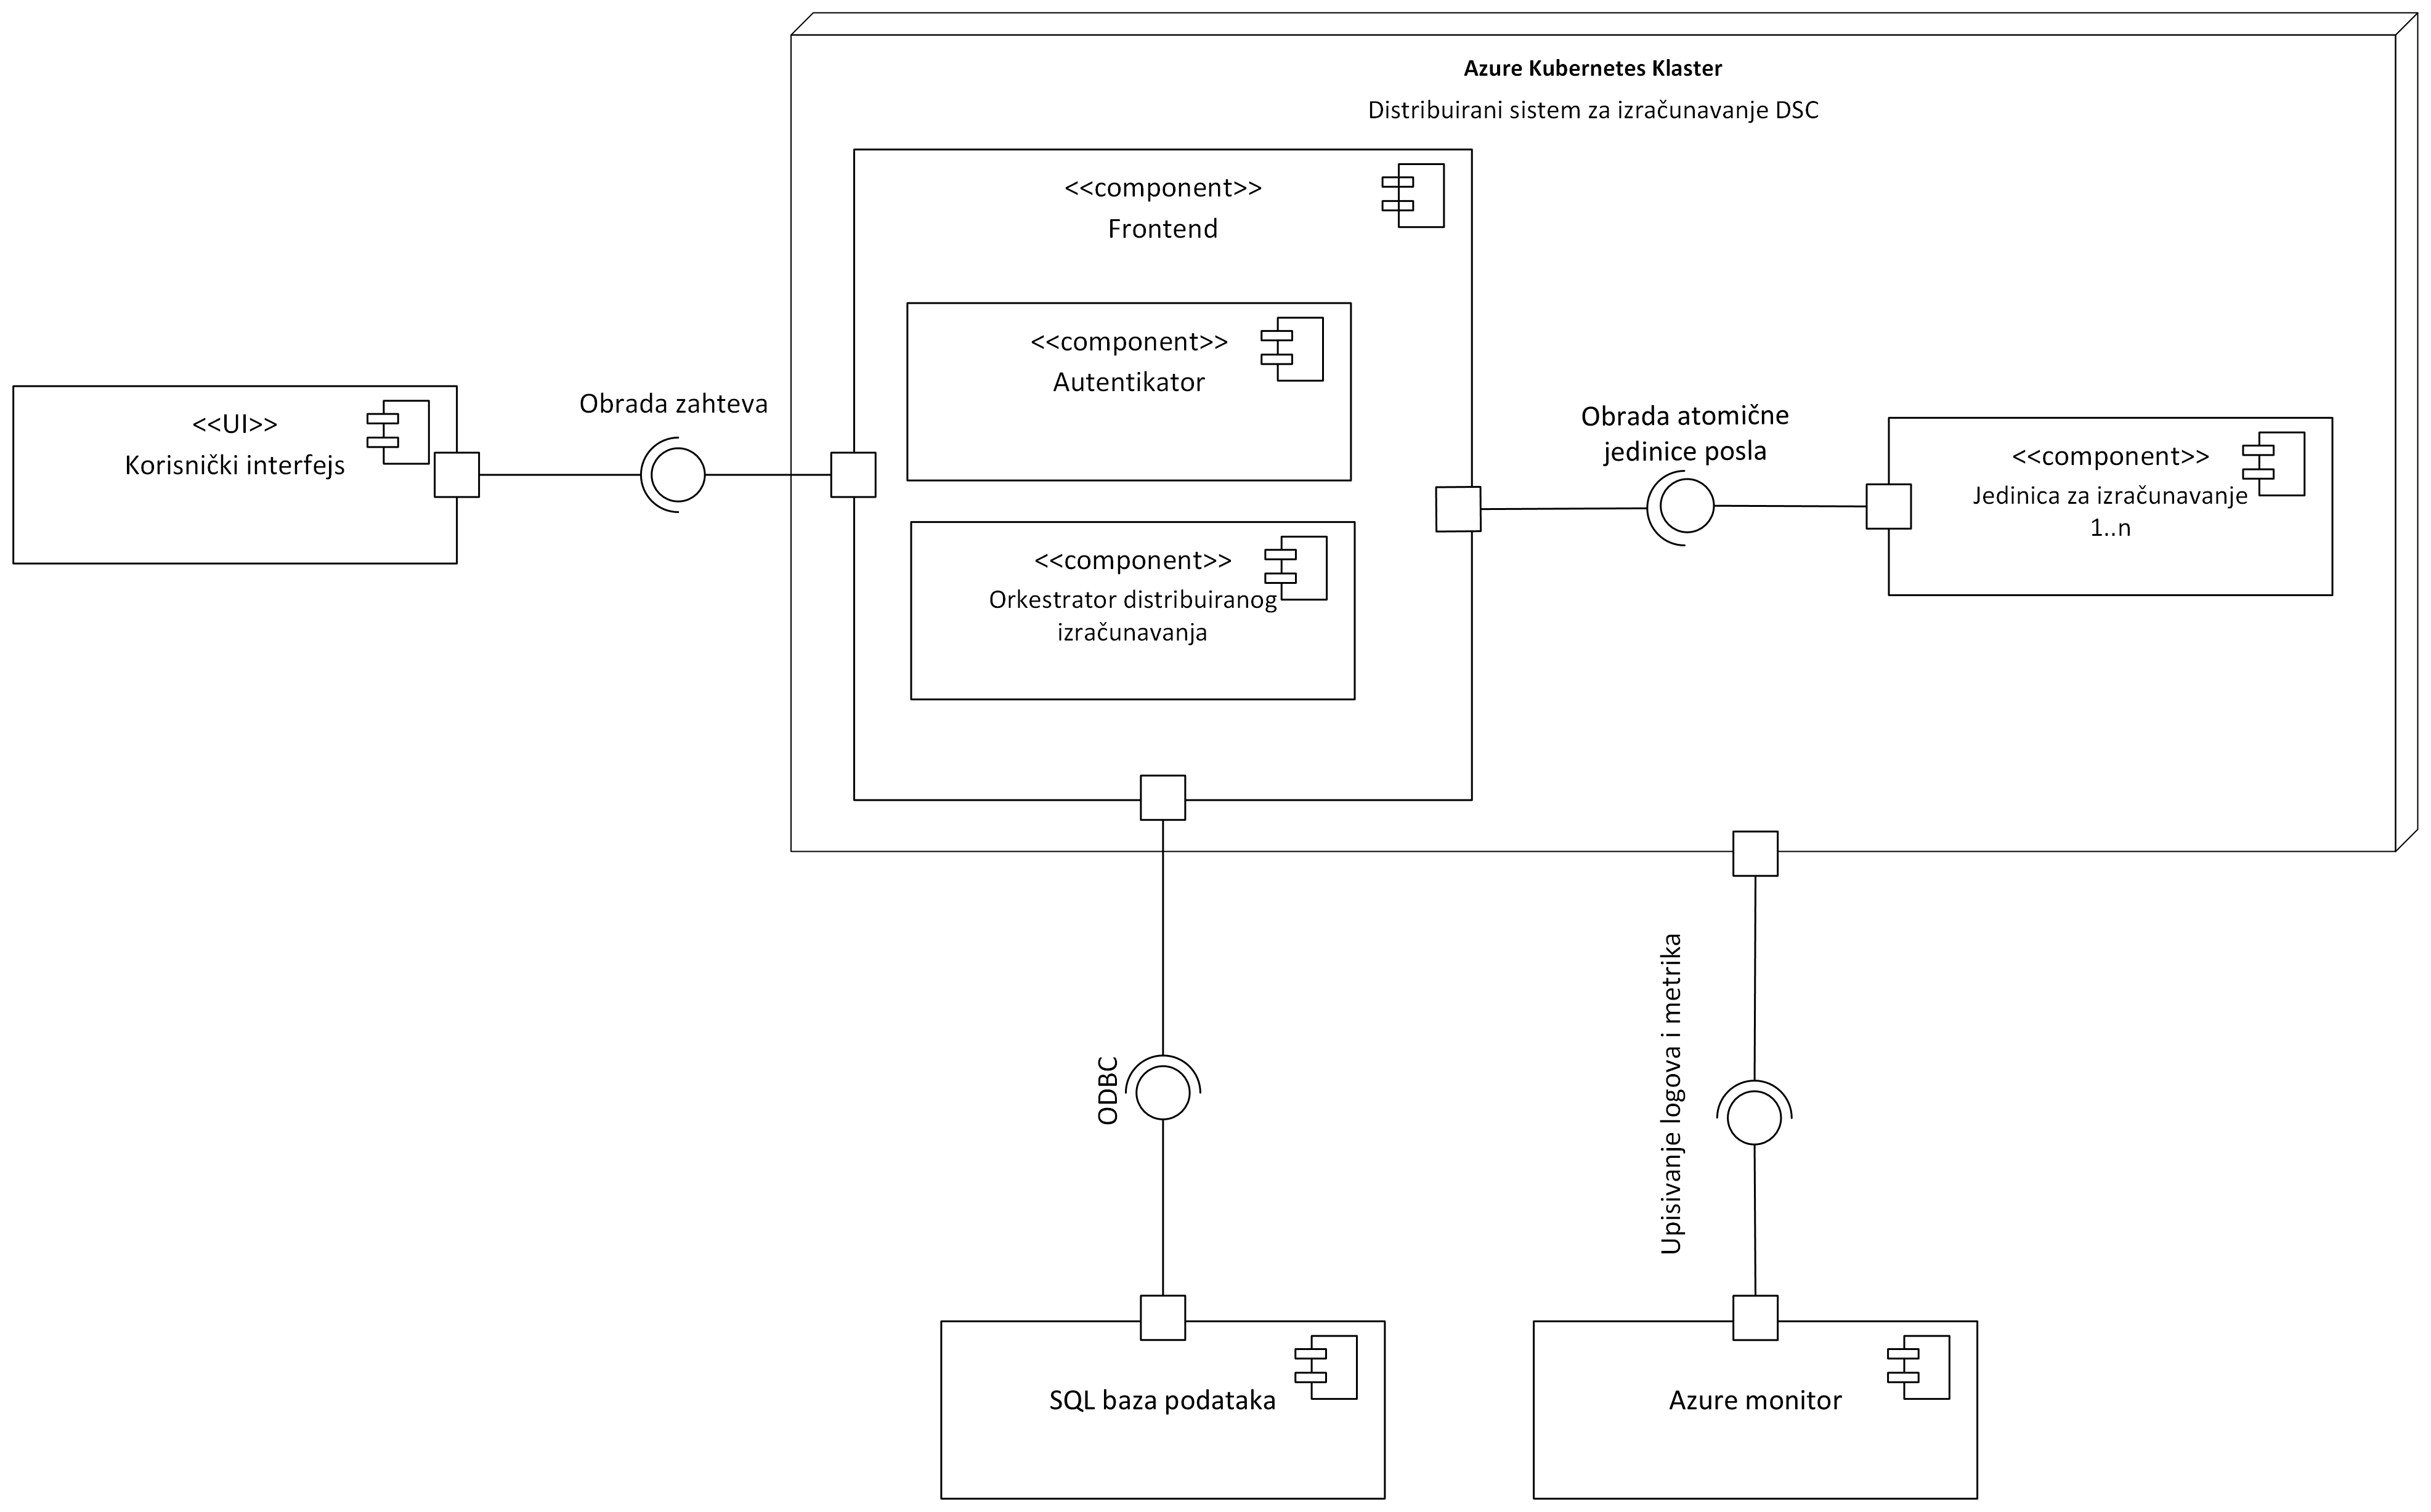
\includegraphics[width=1.0\textwidth]{./images/arhitektura_sistema_dijagram_komponenti.png}
  \caption{UML dijagram komponenti - Arhitektura sistema}
  \label{fig:arhitektura}
\end{figure}

Arhitekturalni obrazac korišćen prilikom razvoja sistema je Prezentacija-Apstrakcija-Kontrola (eng. \emph{Presentation-Abstraction-Control}, skr. PAC). Sistem je hijerarhijski podeljen na agente CtrlN i CmpN. CtrlN je agent višeg novoa, koji je pozvezan sa CmpN agentima. Ovakvom arhitekturom se uvodi podela odgovornosti različitih delova servisa.

PAC je slojevita arhitektura, te svaki od agenata CtrlN i CmpN ima PAC slojeve. Prvi sloj aplikacija je \emph{prezenter} koji predstavlja \emph{REST API}. Ovaj sloj aplikacije je okrenut ka spolja i definiše interfejs za komunikaciju sa servisom. U slučaju CtrlN, to je \emph{API} preko kog prima korisnikove zahteve, a u slučaju CmpN, to je \emph{API} preko kog prima zahteve od CtrlN. Drugi sloj aplikacija je \emph{kontroler} koji predstavlja centralni deo agenta. U okviru kontrolera se nalazi glavna logika. Treći sloj aplikacija je \emph{apstrakcija} i predstavlja model podataka i interfejs prema bazi podataka. 


% ------------------------------------------------------------------------------
\section{Implementacija}
\label{sec:implementacija}
% ------------------------------------------------------------------------------

Sistem DCS je javno dostupan na servisu \emph{GitHub} na adresi \href{https://github.com/milana-kovacevic/DistributedComputationSystem}{https://github.com/milana-kovacevic/DistributedComputationSystem}\label{githubdcs}. Za implementaciju je korišćen programski jezik C\#, i radni okvir \emph{.NET Core 6.0}. Korišćeno je razvojno okruženje \emph{Microsoft Visual Studio Community 2022} i operativni sistem \emph{Windows 10}.

Glavna logika distribuiranog izvršavanja nalazi se u okviru kontrolne jedinice. Jedinice za izvršavanje su jednostavni servisi koji imaju jasan cilj koji podrazumeva izvršavanje atomičnog posla i vraćanje rezultata izvršavanja. U nastavku, razrađuje se implementacija CtrlN komponente (ukoliko nije naglašeno drugačije).

Kontrolna jedinica se sastoji od dve komponente koje se nazivaju: \emph{Frontend} (skr. FE) i Orkestrator distribuiranja (skr. DO). Detaljnije, zaduženja CtrlN su, redom:
\begin{enumerate}
\item \emph{Frontend}
	\begin{enumerate}
	\item Autentifikacija klijenta,
	\item Primanje i validacija zahteva,
	\end{enumerate}
\item Orkestrator distribuiranja
	\begin{enumerate}
	\item \label{podela_planiranje}Podela zahteva na potposlove i pravljenje plana izvršavanja,
	\item \label{orkestriranje}Orkestiranje izvršavanja potposlova i agregacija podrezultata,
	\item \label{cuvanje_u_bazi}Čuvanje rezultata u bazi ili nekom drugom skladištu.
	\end{enumerate}
\end{enumerate}

Moguća stanja kroz koja prolazi posao su prikazana na slici \ref{fig:stanjaposla}, a u nastavku je objašnjen način njegove obrade.

\begin{figure}[!ht]
  \centering
  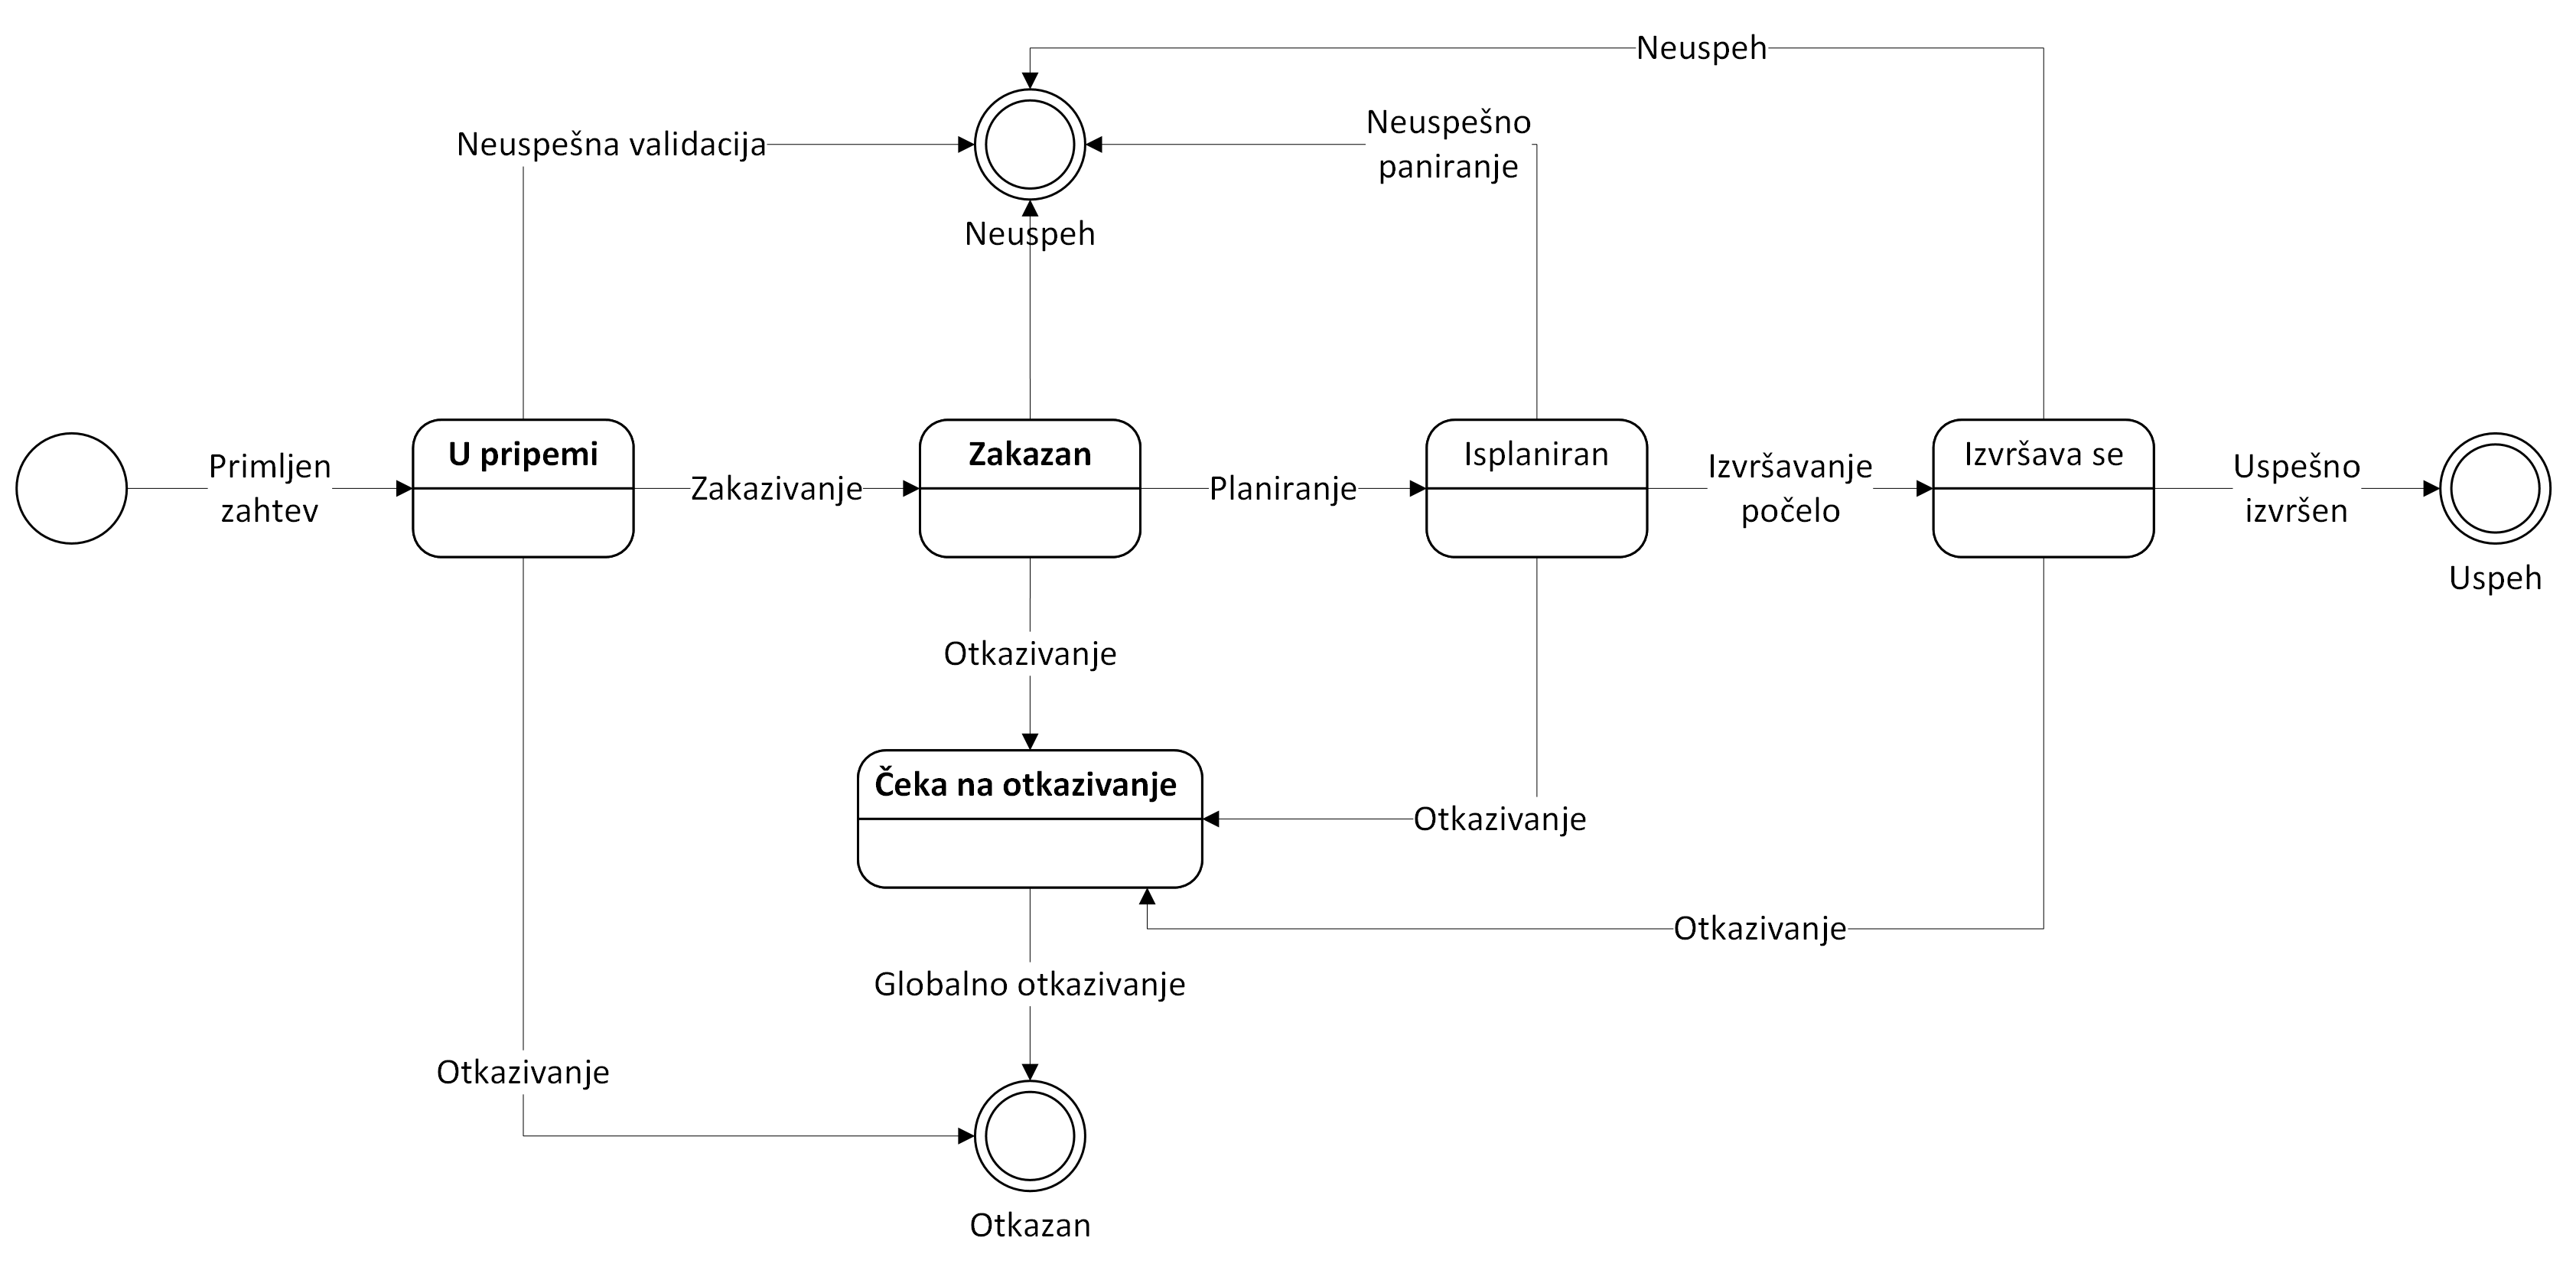
\includegraphics[width=1.0\textwidth]{./images/dijagram_stanja_posao.png}
  \caption{UML dijagram stanja - Posao}
  \label{fig:stanjaposla}
\end{figure}

Kada je FE primio i evidentirao zahtev za izvršavanje posla, on ubacuje posao u red za izvršavanje. U slučaju da je sistem zauzet obradom drugih poslova, novi zahtev će čekati dok sistem ne postane spreman da ga obradi. Za implementaciju reda za čekanje, korišćeno je postojeće rešenje bezbedno pri radu sa nitima \emph{BlockingCollection} \cite{BlockingCollection}. Posebna nit aplikacije uzima poslove iz reda i šalje ih, jednog po jednog, na dalju obradu komponenti DO.

Navedena zaduženja \ref{podela_planiranje} i \ref{orkestriranje} uključuju glavni deo logike distribuiranog izvršavanja. Pre nego što se počne sa izvršavanjem, neophodno je podeliti posao na potposlove i definisati njihove zavisnosti. Rezultat ovoga je predstavljen u vidu stabla u kojem listovi predstavljaju početne atomične poslove, unutrašnji čvorovi agregacije podrezultata, a grane prenos međurezultata. Koren predstavlja krajnje rešenje. U slučaju da korisnikov zahtev već sadrži niz atomičnih poslova, podela početnog zahteva je trivijalna. Na osnovu stabla zavisnosti, pravi se plan izvršavanja. Sličan način planiranja koriste baze podataka \cite{SQLServerInternals}, kao i sistemi poput Sparka \cite{Spark} predstavljen u odeljku \ref{sub:postojeca_resenja}. Plan izvršavanja zavisi od tipa posla, a u slučaju \emph{map-reduce} funkcionalnosti podrazumeva se da se svaki atomični posao nezavisno obrađuje (funkcijom \emph{map}), a krajnje rešenje se dobija definisanom agregacijom atomičnih rezultata (funkcijom \emph{reduce}). Na osnovu plana izvršavanja, komponenta DO sprovodi dalje izvršavanje posla: šalje atomične poslove preko mreže do izabranih CmpN na izvršavanje. Klijent korišćen za komunikaciju između komponenti je generisan pomoću skupa alata \emph{Swagger} opisanih u odeljku \ref{sub:dodatnialati}. Zakazivanje i izvršavanje atomičnih poslova se dešava asinhrono i ono ne blokira DO da uzme naredni posao iz reda i započne njegovu obradu. Dobijeni rezultati se šalju odvojenoj komponenti koja zna da agregara rezultate na osnovu plana izvršavanja. U zavisnosti od kompleksnosti agregacije, i ona može da se prosledi CmpN na izračunavanje.

DO dodatno prati uspešnost izvršavanja poslova i u slučaju uspešnog završetka, upisuje rezultat u bazu. Ukoliko dođe do greške prilikom izvršavanja, posao može da se ponovi ili da se evidentira greška u krajnjem rezultatu. Ponovno pokretanje poslova je potrebno kako bi se povećao stepen pouzdanosti izvršavanja. U distribuiranim sistemima treba imati u vidu da često može doći do problema u komunikaciji među servisima, bilo zbog preopterećenosti mreže ili eventualnih restarta individualnih aplikacija. Ovo može uzrokovati prolaznu grešku, koju je moguće prevazići novim pokušajem. Ukoliko i nakon ponovnog izvršavanja dođe do greške, posao se završava i kao krajnji rezultat se upisuje greška.

Klijent ima mogućnost da otkaže aktivan posao. Ova operacija uključuje i otkazivanje svih njegovih potposlova koji su u procesu izvršavanja ili koji čekaju na izvršavanje, te se ukupno otkazivanje dešava globalno u celom sistemu.
Kada zahtev za otkazivanje stigne do komponente DO, on proverava status posla i status njegovih potposlova. Ukoliko u tom trenutku postoji barem jedan atomični posao koji čeka na izvršavanje ili se izvršava, DO prekida dalje zakazivanje i asinhrono otkazuje poslove koji su u toku izvršavanja. Tada se ažurira status posla i čeka se da se otkažu svi atomični poslovi. Kada sistem globalno otkaže sva izvršavanja, posao je otkazan i klijentu se vraća potvrda o uspešnosti.

%TODO dijagram klasa DO

\subsection{Baza podataka}

Sistem DCS koristi relacionu bazu podataka za evidentiranje poslova. DCS ažurira stanja u kojem se nalazi posao kako bi korisnik mogao da prati šta se dešava u sistemu. Dodatno, baza podataka služi i za čuvanje rezultata i međurezultata poslova.

ER (eng. \emph{Entity-Relation}) dijagram modela posla je prikazan na slici \ref{fig:erposao}.

\begin{figure}[!ht]
  \centering
  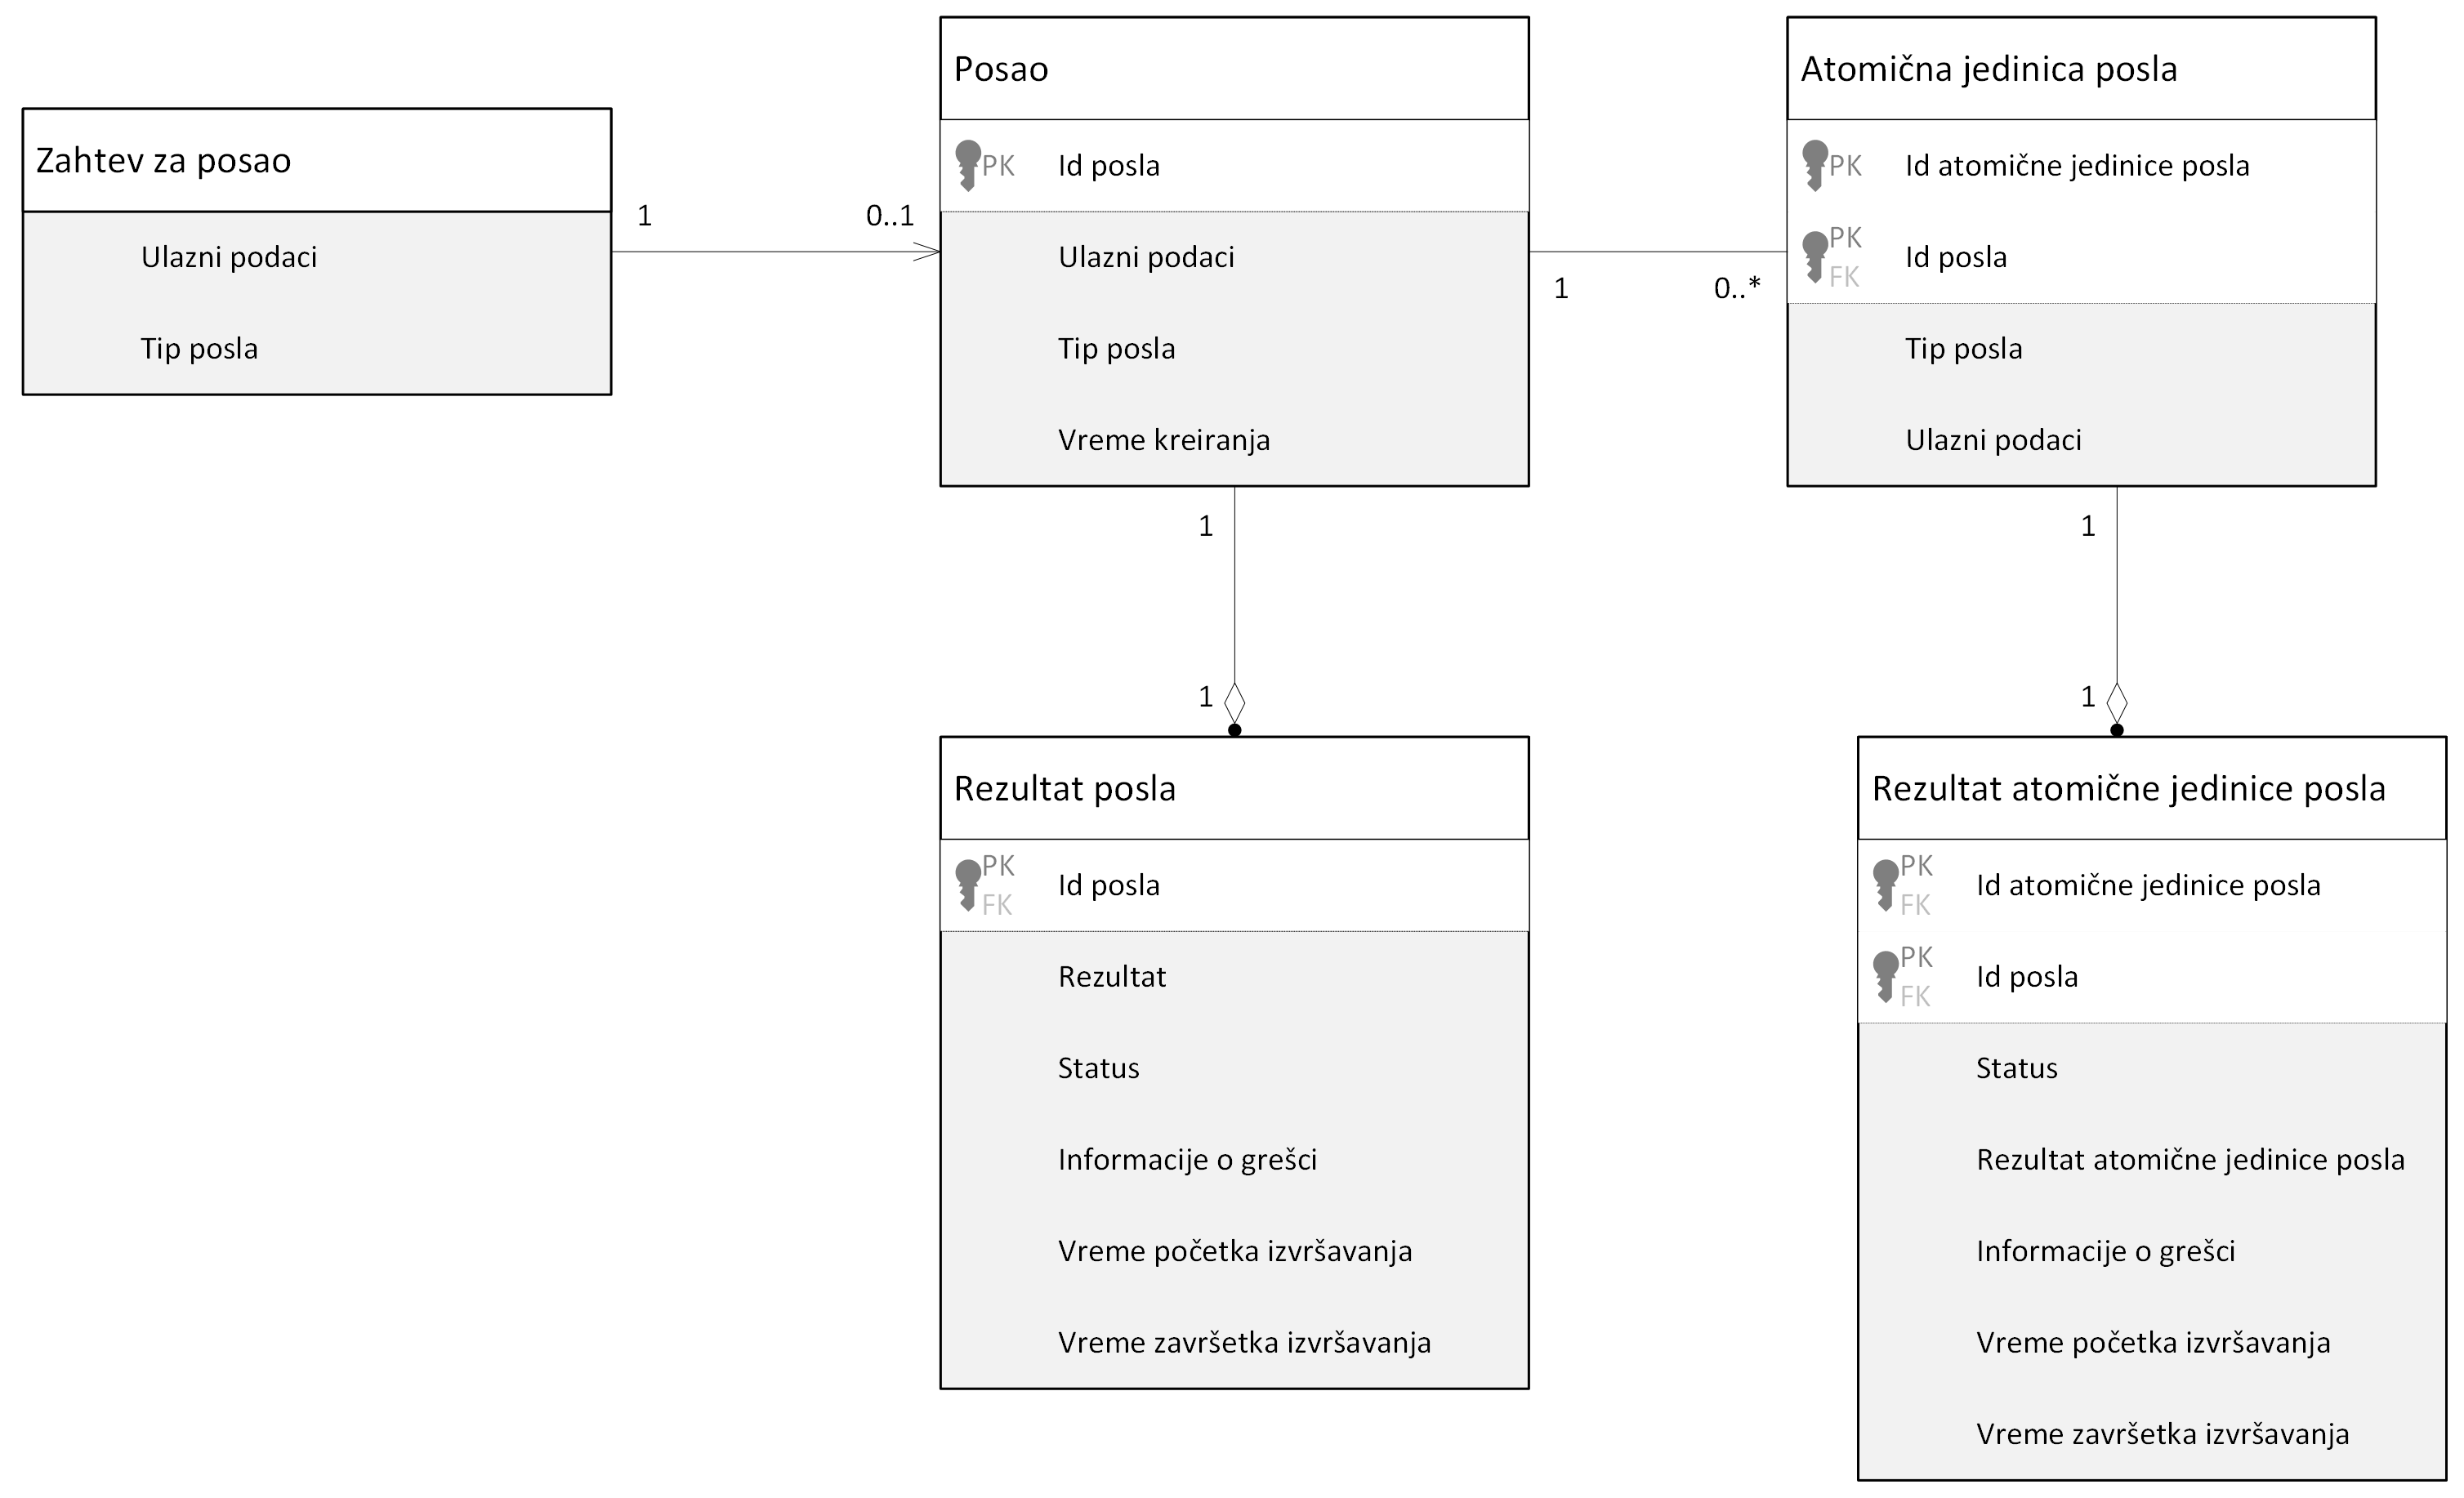
\includegraphics[width=1.0\textwidth]{./images/uml_er_dijagram_posao.png}
  \caption{ER dijagram entiteta u bazi podataka}
  \label{fig:erposao}
\end{figure}


\subsection{Autentifikacija}

Za autentifikaciju klijenta je korišćen servis \emph{AAD} \cite{AAD} opisan u uvodnom poglavlju u odeljku \ref{sub:azureplatform}. Korisniku su dodeljena prava korišćenja servisa time što je njegov identitet, član grupe korisnika definisane u okviru servisa AAD.

Proces autentifikacije je prikazan na slici \ref{fig:autentifikacija}. Korisnik pre kontaktiranja sistema DCS šalje zahtev servisu \emph{AAD} kako bi preuzeo token za autentifikaciju. Ovaj token ima rok trajanja (uobičajeno je 60 minuta) i specifičan je za autentifikaciju na DCS sistem. Kada klijent ima token, prosleđuje ga u \emph{header} delu \emph{http} zahteva u polju za autentifikaciju. Sistem DCS prima zahtev i pre nego što počne da ga obrađuje, izvrši validaciju \emph{AAD} tokena. Token sadrži otisak (eng. \emph{thumbprint}) koji garantuje njegovu validnost. Ukoliko je token ispravan, nastavlja se sa obradom zahteva, a ukoliko nije, korisnikov zahtev se odbija uz odgovarajuću grešku.

Za bezbednu komunikaciju u produkcionom okruženju, korišćen je protokol \emph{https}.

\begin{figure}[!ht]
  \centering
  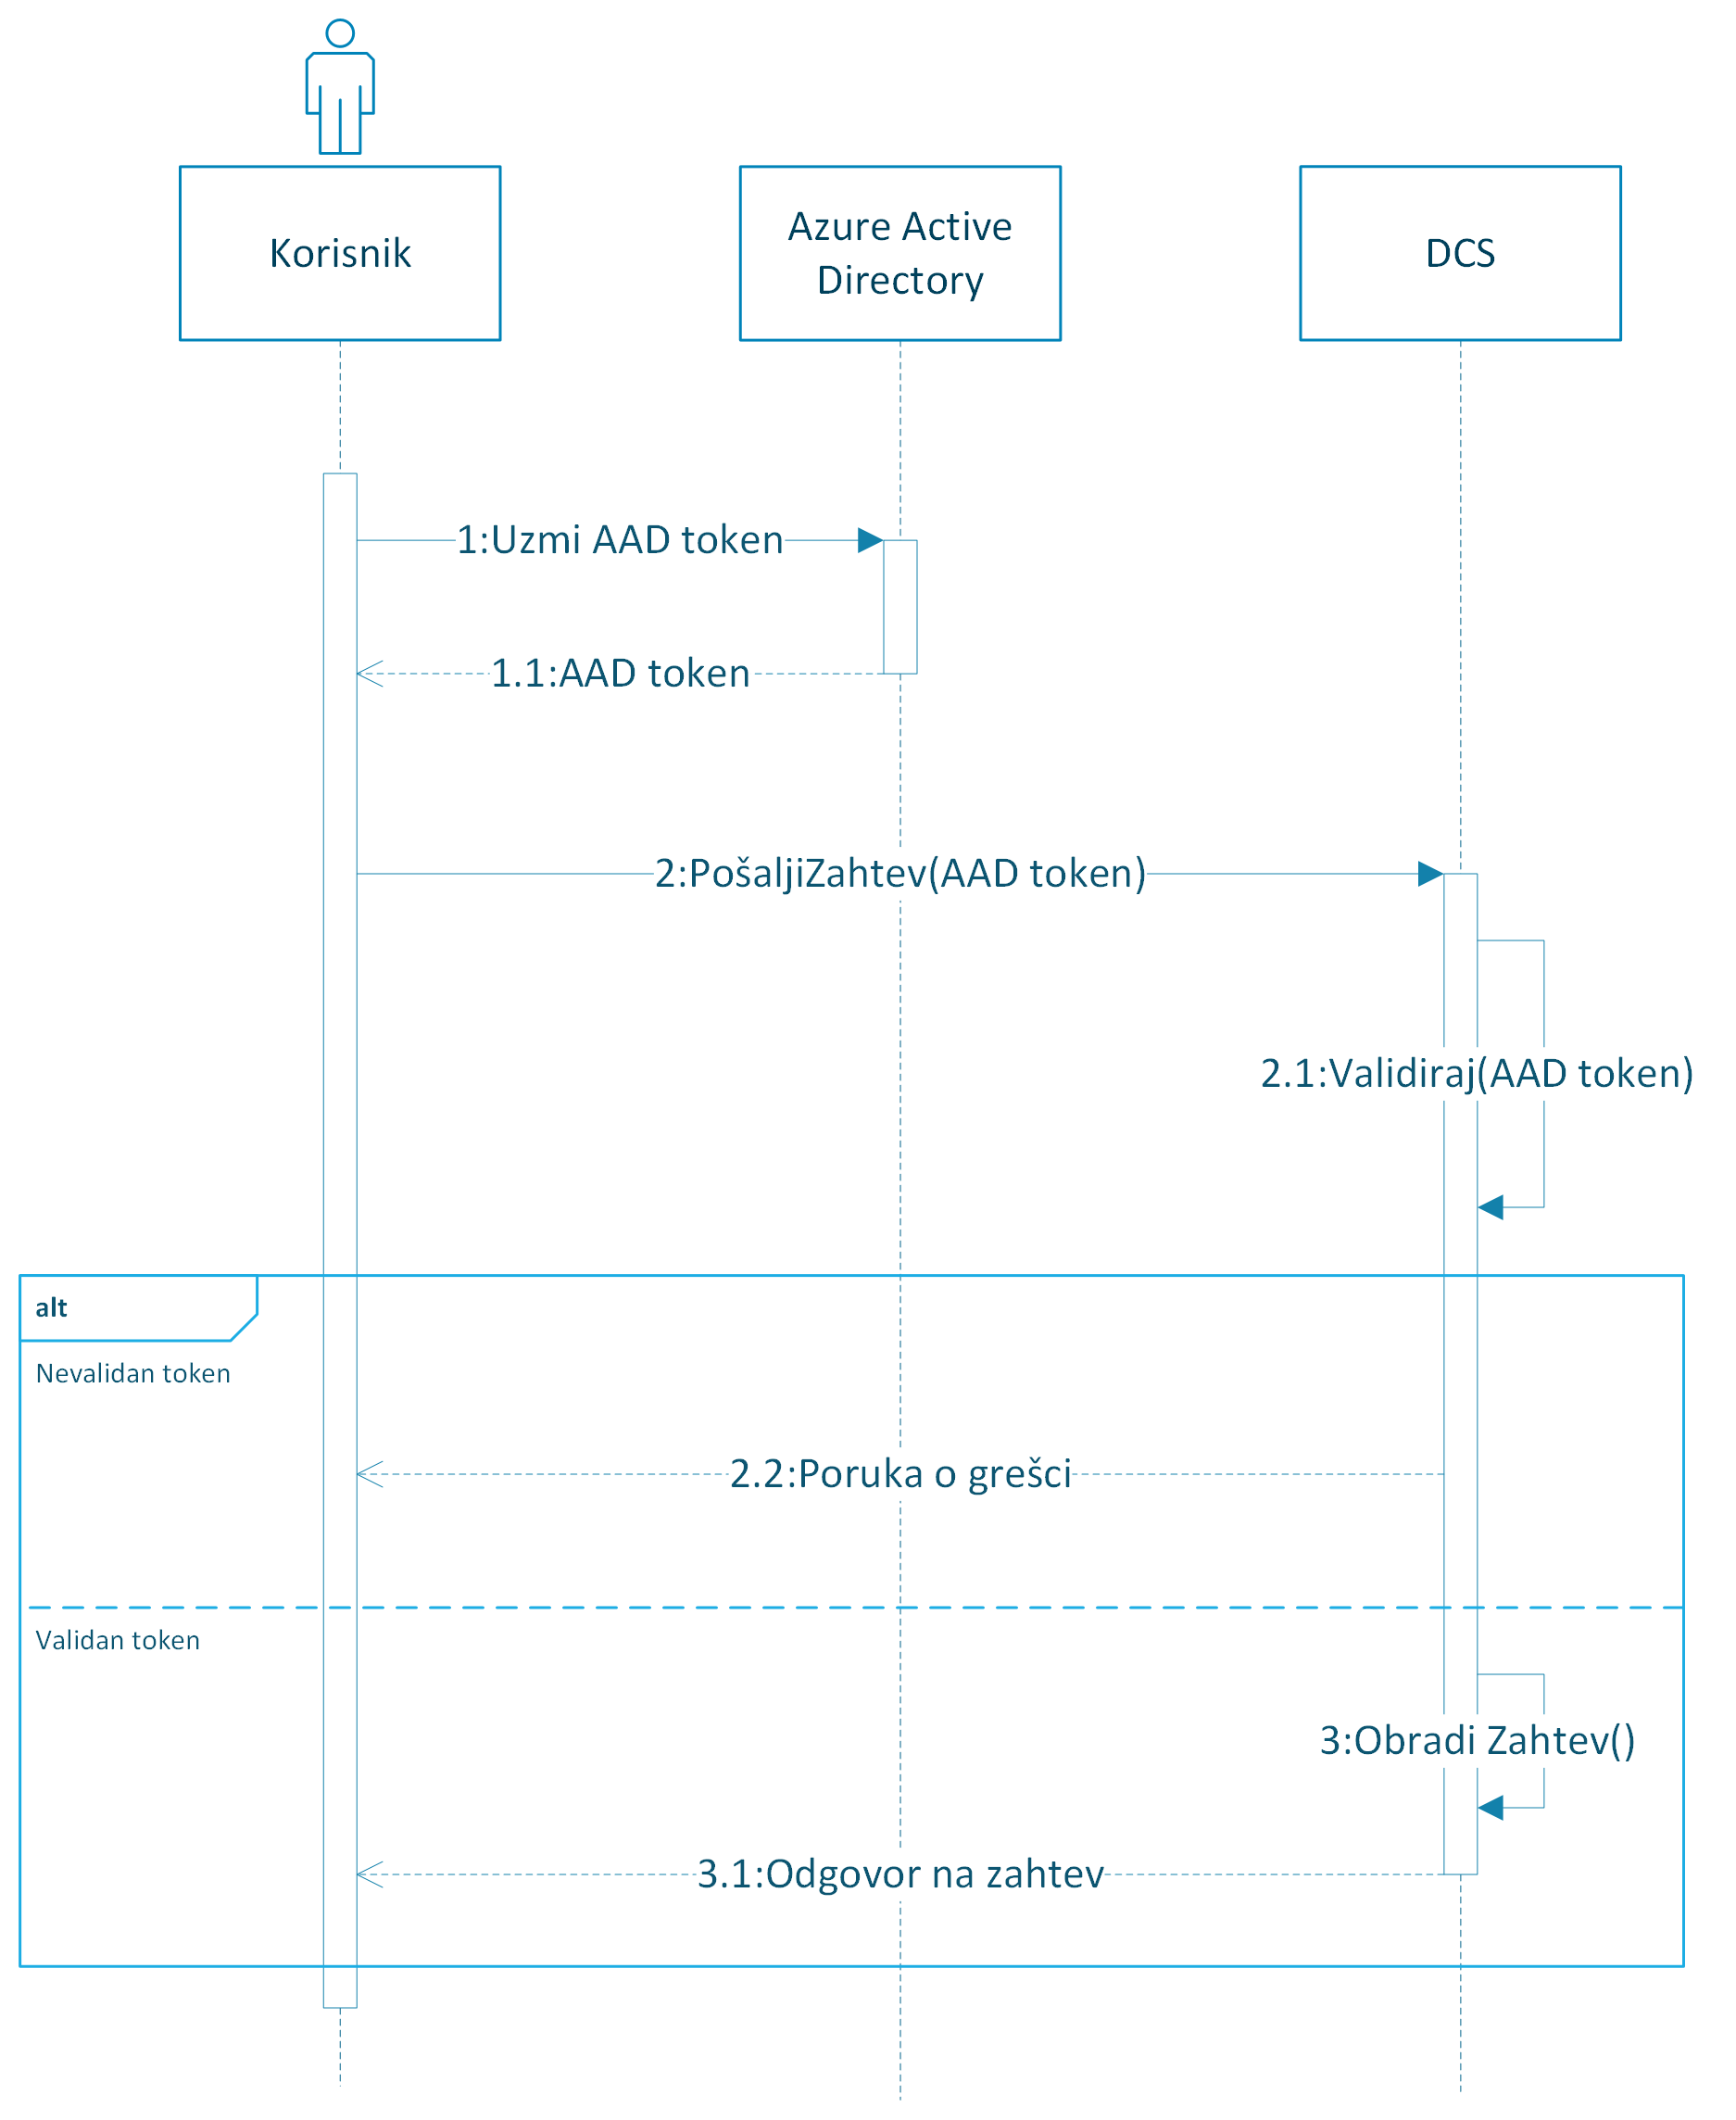
\includegraphics[width=1.0\textwidth]{./images/autentikacija_uml_dijagram_sekvence.png}
  \caption{UML dijagram sekvence - Autentifikacija}
  \label{fig:autentifikacija}
\end{figure}


\section{Pokretanje u oblaku}

Opisana implementacija dobija smisao i punu moć pokretanjem sistema DCS na klasteru Kubernetes predstavljenom u uvodu u delu \ref{subs:kubernetes_platform}. Komponente \emph{Control Node} i \emph{Compute Node} se pokreću u okviru \emph{Docker} kontejnera (uvodni deo, odeljak \ref{subs:docker_platform}). Izbor radnog okvira \emph{.NET Core} omogućava pokretanje servisa na različitim platformama \emph{Windows}, \emph{Mac} i \emph{Linux}, bez izmena izvornog koda. Za izradu sistema su korišćeni \emph{Docker}kontejneri sa operativnim sistemom \emph{Linux}. Za pokretanje sistema DCS u oblaku je korišćena platforma \emph{Microsoft Azure} \cite{Azure}. Za upravljanje i pristup resursima u okviru ove platforme koristi se portal \emph{Azure} \cite{AzurePortal}.

Na adresi projekta na servisu \emph{GitHub} \ref{githubdcs} se nalaze datoteke potrebne za kreiranje i konfigurisanje servisa pokrenutih u okviru klastera Kubernetes, kao i pomoćne skripte koje automatizuju proces postavljanja nove verzije aplikacija na klaster.

U nastavku, na slici \ref{fig:controlnode_yaml} je prikazana datoteka u formatu \emph{yaml} koja definiše kreiranje aplikacije \emph{Control Node} na klasteru Kubernetes.

\begin{figure}[h!]
\centering
\begin{lstlisting}[style=yaml]
apiVersion: apps/v1
kind: Deployment
metadata:
  name: controlnode
  namespace: distributed-system-dev-ns
  labels:
    app: controlnode
spec:
  replicas: 1
  selector:
    matchLabels:
      app: controlnode
  strategy: {}
  template:
    metadata:
      labels:
        app: controlnode
    spec:
      containers:
        - name: controlnode-container
          image: matfmastercr.azurecr.io/controlnode:v1.1
          imagePullPolicy: IfNotPresent
          ports:
            - containerPort: 80
              protocol: TCP
          env:
            - name: ASPNETCORE_URLS
              value: http://+:80
\end{lstlisting}
\caption{Definisanje kreiranja aplikacije \emph{Control Node}}
\label{fig:controlnode_yaml}
\end{figure}

Kako bi se efikasno pristupalo aplikaciji preko mreže, kreira se i odgovarajući servis koristeći datoteku u formatu \emph{yaml} prikazanu na slici \ref{fig:controlnode_service_yaml}. Tada je moguće pristupiti servisu koristeći njegovo ime ili dodeljenu statičku adresu servisa.

\begin{figure}[h!]
\centering
\begin{lstlisting}[style=yaml]
apiVersion: v1
kind: Service
metadata:
  name: controlnode
  namespace: distributed-system-dev-ns
  labels:
    app: controlnode
spec:
  type: ClusterIP
  ports:
  - port: 80
    name: 80-80
    protocol: TCP
    targetPort: 80
  selector:
    app: controlnode
  internalTrafficPolicy: Local
\end{lstlisting}
\caption{Definisanje kreiranja servisa \emph{Control Node}}
\label{fig:controlnode_service_yaml}
\end{figure}

Specifikacije za aplikaciju i servis komponente \emph{Compute Node} su analogne, s tim da on može imati i više od jedne replike. Kreiranjem servisa CmpN, omogućava se da CtrlN komunicira prema njemu koristeći samo poznatu \emph{IP} adresu servisa. Ova adresa se ne menja tokom postojanja servisa, a klaster Kubernetes automatski usmerava zahteve prema dostupnim, odgovarajućim mahunama, tj. kontejnerima. Više o ovome se nalazi u odeljku \ref{subs:kubernetes_platform}. Na ovaj način, sistem DCS se oslanja na postojeći mehanizan balansiranja saobraćaja u okviru klastera. Iz ugla CtrlN, on uvek šalje zahteve na jednu adresu CmpN, a tu adresu čita iz promenljive postavljene u okruženje (eng. \emph{environment variable}).

Servisi su definisani tako da primaju samo lokalni saobraćaj, odnosno saobraćaj u okviru mreže klastera. Koriste lokalni port 80, što je standardni port za http, a smatra se da je komunikacija unutar klastera bezbedna. CtrlN je potrebno otvoriti prema korisniku putem interneta, odnosno, dodeliti mu javnu \emph{IP} adresu, što je moguće uraditi na više načina. Jedan od načina je kreiranjem servisa tipa \emph{LoadBalanser}, koji mu automatski dodeljuje eksternu \emph{IP} adresu. Međutim, ovaj način dodeljivanja adrese komplikuje podešavanja bezbednosnog protokola \emph{https}, koji zahteva instalaciju sertifikata \emph{TLS} na serverskoj mašini. Zbog ovoga je kreiran dodatni \emph{API} objekat koji se naziva \emph{Ingress}, a način njegovog kreiranja je prikazan na slici \ref{fig:controlnode_ingress_yaml}. Ovaj objekat predstavlja vezu između spoljašnjosti i unutrašnjosti klastera. Dodeljena mu je statička \emph{IP} adresa sa uvezanim \emph{DNS} imenom, koji su prethodno kreirani preko portala. Ovaj objekat takođe usmerava zahteve ka željenim servisima na osnovu definisanih pravila. U sučaju DCS, sve zahteve (označene prefiksom /) usmerava na CtrlN. Za instaliranje i automatsko rotiranje sertifikata, kreiran je i objekat \emph{ClusterIssuer}, koji koristi javnog snabdevača \emph{TLS} sertifikatima, \emph{Let's encrypt} \cite{letsencrypt}. Uz ovakvo podešavanje, produkcionom sistemu DCS se može pristupiti preko javno dostupne adrese \emph{matf-distr-comp-sys.westeurope.cloudapp.azure.com} koristeći \emph{https}.

\begin{figure}[h!]
\centering
\begin{lstlisting}[style=yaml]
apiVersion: networking.k8s.io/v1
kind: Ingress
metadata:
  name: cn-tls
  namespace: distributed-system-dev-ns
  annotations:
    nginx.ingress.kubernetes.io/ssl-redirect: "false"
    cert-manager.io/cluster-issuer: letsencrypt
spec:
  ingressClassName: nginx
  tls:
  - hosts:
    - matf-distr-comp-sys.westeurope.cloudapp.azure.com
    secretName: tls-secret
  rules:
  - host: matf-distr-comp-sys.westeurope.cloudapp.azure.com
  - http:
      paths:
      - path: /
        pathType: Prefix
        backend:
          service:
            name: controlnode
            port:
              number: 80
\end{lstlisting}
\caption{Kreiranje objekta ingress za pristup CtrlN preko \emph{DNS} imena i \emph{https} protokola}
\label{fig:controlnode_ingress_yaml}
\end{figure}

Broj mahuna aplikacije CmpN je moguće automatski skalirati kreiranjem \emph{autoscale} objekta. Komanda koja skalira broj CmpN u odnosu na procenat iskorišćenosti procesora je sledeća:

\begin{verbatim}
kubectl autoscale deployment computenode --cpu-percent=60 --min=2 --max=7 \
 --namespace=distributed-system-dev-ns
\end{verbatim}

% ------------------------------------------------------------------------------
\section{Okvir za testiranje}
\label{sec:testiranjesistema}
% ------------------------------------------------------------------------------

Za izradu testova korišćen je radni okvir \emph{XUnit} \cite{XUnit}.

Svi testovi se nalaze na servisu \emph{GitHub} na adresi projekta u poddirektorijumu \href{https://github.com/milana-kovacevic/DistributedComputationSystem/tree/main/tests}{tests}.

Radni okvir \emph{XUnit} ima podršku za pisanje dva tipa testova: činjenice (eng. \emph{Fact}) i teorije (eng. \emph{Theory}). Činjenice su testovi koji ne primaju argumente, dok teorije predstavljaju parametrizovane testove. Specifikacijom atributa iznad tela funkcije teorijskog testa, definišu se ulazi nad kojima se test pokreće, što značajno olakšava generisanje testova sa različitim ulazima.

Struktura foldera sa testovima je prikazana na slici \ref{fig:testovi}, a na slici \ref{fig:testexplorer} se nalazi vizuelni prikaz rezultata izvršavanja testova u okruženju \emph{Microsoft Visual Studio}.

\begin{figure}[!ht]
  \centering
  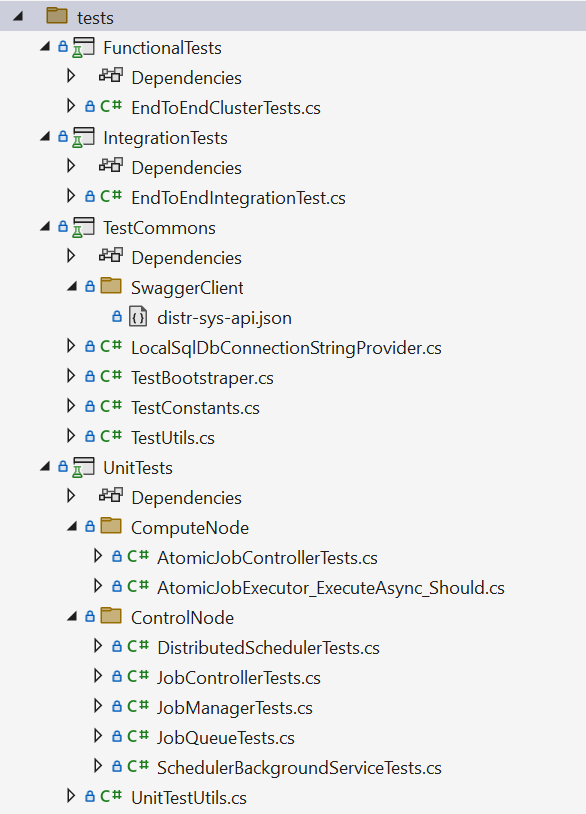
\includegraphics[width=0.8\textwidth]{./images/testovi.png}
  \caption{Struktura foldera sa testovima}
  \label{fig:testovi}
\end{figure}

\begin{figure}[!ht]
  \centering
  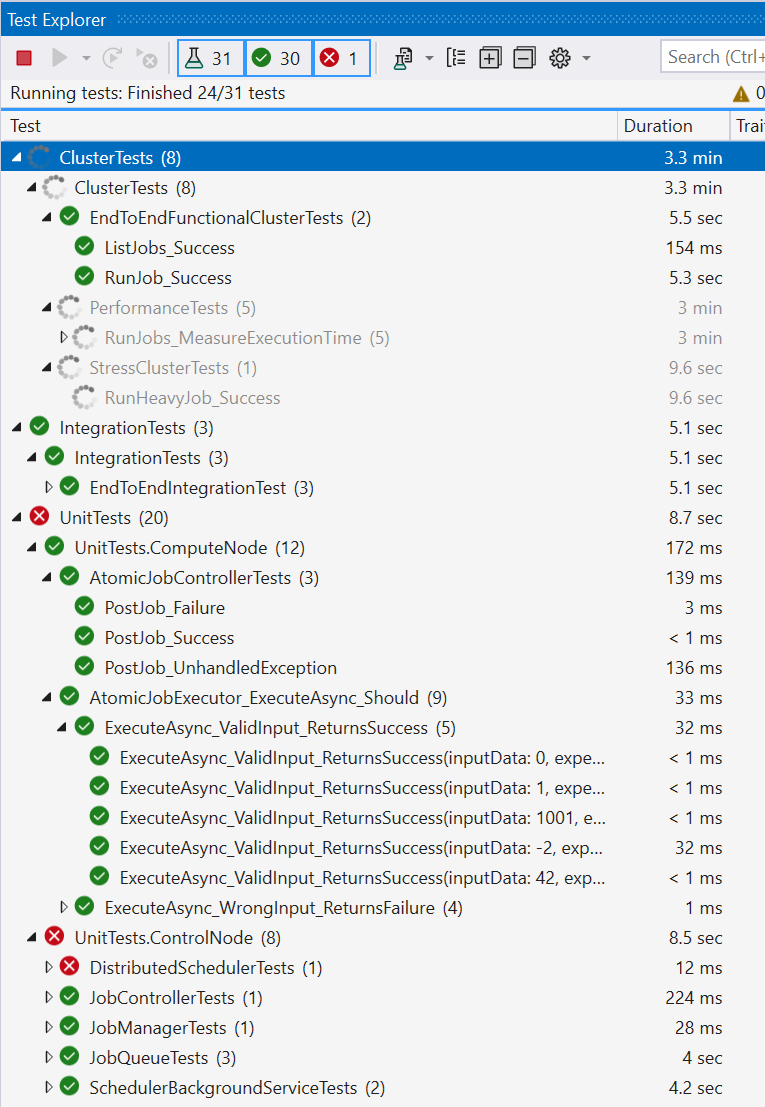
\includegraphics[width=0.8\textwidth]{./images/testexplorer.png}
  \caption{Pokretanje testova u okruženju \emph{Microsoft Visual Studio}}
  \label{fig:testexplorer}
\end{figure}

Sistem je testiran na više nivoa, počevši od testiranja jedinica koda za svaku komponentu, zatim testova integracije, i, na najvišem nivou, funkcionalnih testova koji ukljucuju klaster testove.

\subsection{Testiranje jedinica koda}
Komponente \emph{Control Node} i \emph{Compute Node} prate odgovarajući testovi jedinica koda. Ovi testovi se nalaze u zasebnom projektu. Tokom izrade testova jedinica koda, korišćen je i radni okvir \emph{Moq} \cite{Moq} za "podmetanje" vrednosti u zavisnim delova koda. U nastavku se nalazi slika \ref{fig:testscheduler} sa primerom testa jedinice koda u okviru komponente CtrlN.

\begin{figure}[h!]
\centering
\begin{lstlisting}
public class DistributedSchedulerTests
{
	private readonly ServiceProvider serviceProvider;
	private readonly Mock<IComputeNodeClientWrapper> mockedComputeNodeClient = new();

	public DistributedSchedulerTests()
	{
		// Configure services using common bootstraper for tests
		var services = new ServiceCollection();
		TestBootstraper.ConfigureServices_Frontend(services);

		// Setup mocked ComputeNodeClient
		mockedComputeNodeClient.Setup(m => m.RunAsync(It.IsAny<int>(), It.IsAny<int>(), It.IsAny<FrontendAtomicJobType>(), It.IsAny<string>()))
			.Returns(Task.FromResult(new FrontendAtomicJobResult()));
		services.AddScoped((services) => mockedComputeNodeClient.Object);

		services.AddScoped<IScheduler, DistributedScheduler>();
		serviceProvider = services.BuildServiceProvider();
	}

	[Fact]
	public async Task ScheduleJobAsync_Success()
	{
		var scheduler = serviceProvider.GetService<IScheduler>();
		Assert.NotNull(scheduler);

		var jobToBeScheduled = UnitTestUtils.GetDummyJob();
		await scheduler.ScheduleJobAsync(jobToBeScheduled);

		mockedComputeNodeClient.Verify(client => client.RunAsync(It.IsAny<int>(), jobToBeScheduled.JobId, It.IsAny<FrontendAtomicJobType>(), It.IsAny<string>()), Times.AtLeastOnce());
		Assert.NotEmpty(scheduler.GetInProgressTasks());
	}
}
\end{lstlisting}
\caption{Primer testa koji koristi radni okvir \emph{Moq}}
\label{fig:testscheduler}
\end{figure}

\subsection{Integracioni testovi}

Postoje dva tipa integracionih testova:
\begin{enumerate}
\item Testovi integracije unutar komponenti,
\item Testovi integracije celih komponenti.
\end{enumerate} 

Testovi integracije unutar komponenti testiraju međusobne zavisnosti podkomponenti CtrlN i CmpN. Na primer, zavisnost FE i DO u okviru CtrlN.

Testovi integracije celih komponenti CtrlN i CmpN se pokreću nad lokalnim okruženjem, i očekuju da je okruženje pripremljeno za njihovo izvšavanje. U okviru \emph{Docker} kontejnera potrebno je pokrenuti jednu CtrlN aplikaciju, kao i jednu CmpN aplikaciju, sa ranije definisanim adresama i portovima. Koristi se automatski generisana klijentska klasa \emph{DistributedComputationSystemClient} nastala korišćenjem alata \emph{Swagger} u toku prevođenja projekta sa testovima. Ovaj klijent šalje zahteve servisu CtrlN, a u telu testova se proverava da li je odgovor od sistema očekivan.

\subsection{Testovi nad klasterom}

Testovi nad klasterom testiraju sistem iz ugla korisnika u produkcionom okruženju. Oni se pokreću nad klasterom u oblaku, i u njima se takođe koristi generisani klijent. Dele se na nekoliko grupa:
\begin{enumerate}
\item Funkcionalni testovi - Testiraju osnovne funkcionalnosti servisa u produkcionom okruženju.
\item Stres-testovi - Skup testova koji se izvršavaju kako bi se analiziralo i unapredilo ponašanje sistema pod opterećenjem. 
\item Testovi performansi - Skup testova koji se pokreću nad servisom pokrenutim u oblaku, sa fokusom na praćenje vremena potrebnog da sistem odradi očekivani posao. Cilj ovog testiranja je uvid u performanse sistema u odnosu na resurse dodeljene klasteru.
\end{enumerate}

Na slici \ref{fig:teste2e} se nalazi primer koji testira funkcionalnost sistema od početka do kraja: zakazivanje posla, preuzimanje statusa, i provera rezultata.

\begin{figure}[h!]
\centering
\begin{lstlisting}
[Fact]
public async void RunJob_Success()
{
	var inputData = new Collection<AtomicJobRequestData>()
	{
		new AtomicJobRequestData() { InputData ="42" },
		new AtomicJobRequestData() { InputData ="142" },
	};
	string expectedTotalSum = "1453";

	var request = new JobRequestData()
	{
		JobType = JobType.CalculateSumOfDigits,
		InputData = inputData
	};

	// Create job.
	var job = await _client.CreateAsync(request);
	Assert.NotNull(job);

	// Verify job is created.
	var jobFromSystem = await _client.JobsAsync(job.JobId);
	Assert.NotNull(jobFromSystem);

	// Poll and verify job state until it's successfully completed.
	await TestUtils.PollUntilSatisfied(
		job.JobId,
		(jobId) =>
		{
			var jobFromSys = _client.JobsAsync(jobId).GetAwaiter().GetResult();
			return jobFromSys.State == JobState.Succeeded;
		},
		timeout: defaultTimeout);

	// Verify aggregated result.
	var jobResult = await _client.JobResultsAsync(job.JobId);
	Assert.Equal(string.Empty, jobResult.Error);
	Assert.Equal(expectedTotalSum, jobResult.Result);
	Assert.Equal(JobState.Succeeded, jobResult.State);

	// Delete job.
	await _client.DeleteAsync(job.JobId);

	// Now getting job should throw 404.
	var exception = Assert.ThrowsAsync<ApiException>(async () => await _client.JobsAsync(job.JobId));
	Assert.Equal<int>((int)HttpStatusCode.NotFound, exception.Result.StatusCode);
}
\end{lstlisting}
\caption{Primer funkcionalnog testa}
\label{fig:teste2e}
\end{figure}

Stres-testovi i testovi performansi ispituju granice sistema. Oni su neophodni kako bi se na vreme razumela i unapredila uska grla sistema, kao i da bi se razumele mogućnosti sistema u skladu sa dodeljenim resursima.


% ------------------------------------------------------------------------------
\section{Praćenje rada sistema}
\label{chp:pracenjemetrika}
% ------------------------------------------------------------------------------

U ovom odeljku su prikazane mogućnosti praćenja rada sistema uz pomoć servisa \emph{Azure Monitor} za praćenje ponašanja resursa u oblaku. Kako su glavne komponente sistema pokrenute u okviru klastera \emph{Azure Kubernetes Service}, dat je pregled načina na koji se analiziraju podaci o radu klastera. Na analogan način se može pratiti i ponašanje baze podataka \emph{Azure SQL Database} koju koristi sistem.

\subsection{Metrike}

Metrike sistema predstavljaju koncizne informacije o njegovom radu u (skoro) realnom vremenu. Kroz metrike možemo da vidimo trenutnu iskorišćenost resursa klastera, status mašina, mahuna, kontejnera, itd.

Na slici \ref{fig:aksinsights} je prikazan pogled na sekciju \emph{Insight} pripadajućeg klastera kojem se pristupa preko portala \cite{AzurePortal}.

\begin{figure}[!ht]
  \centering
  \frame{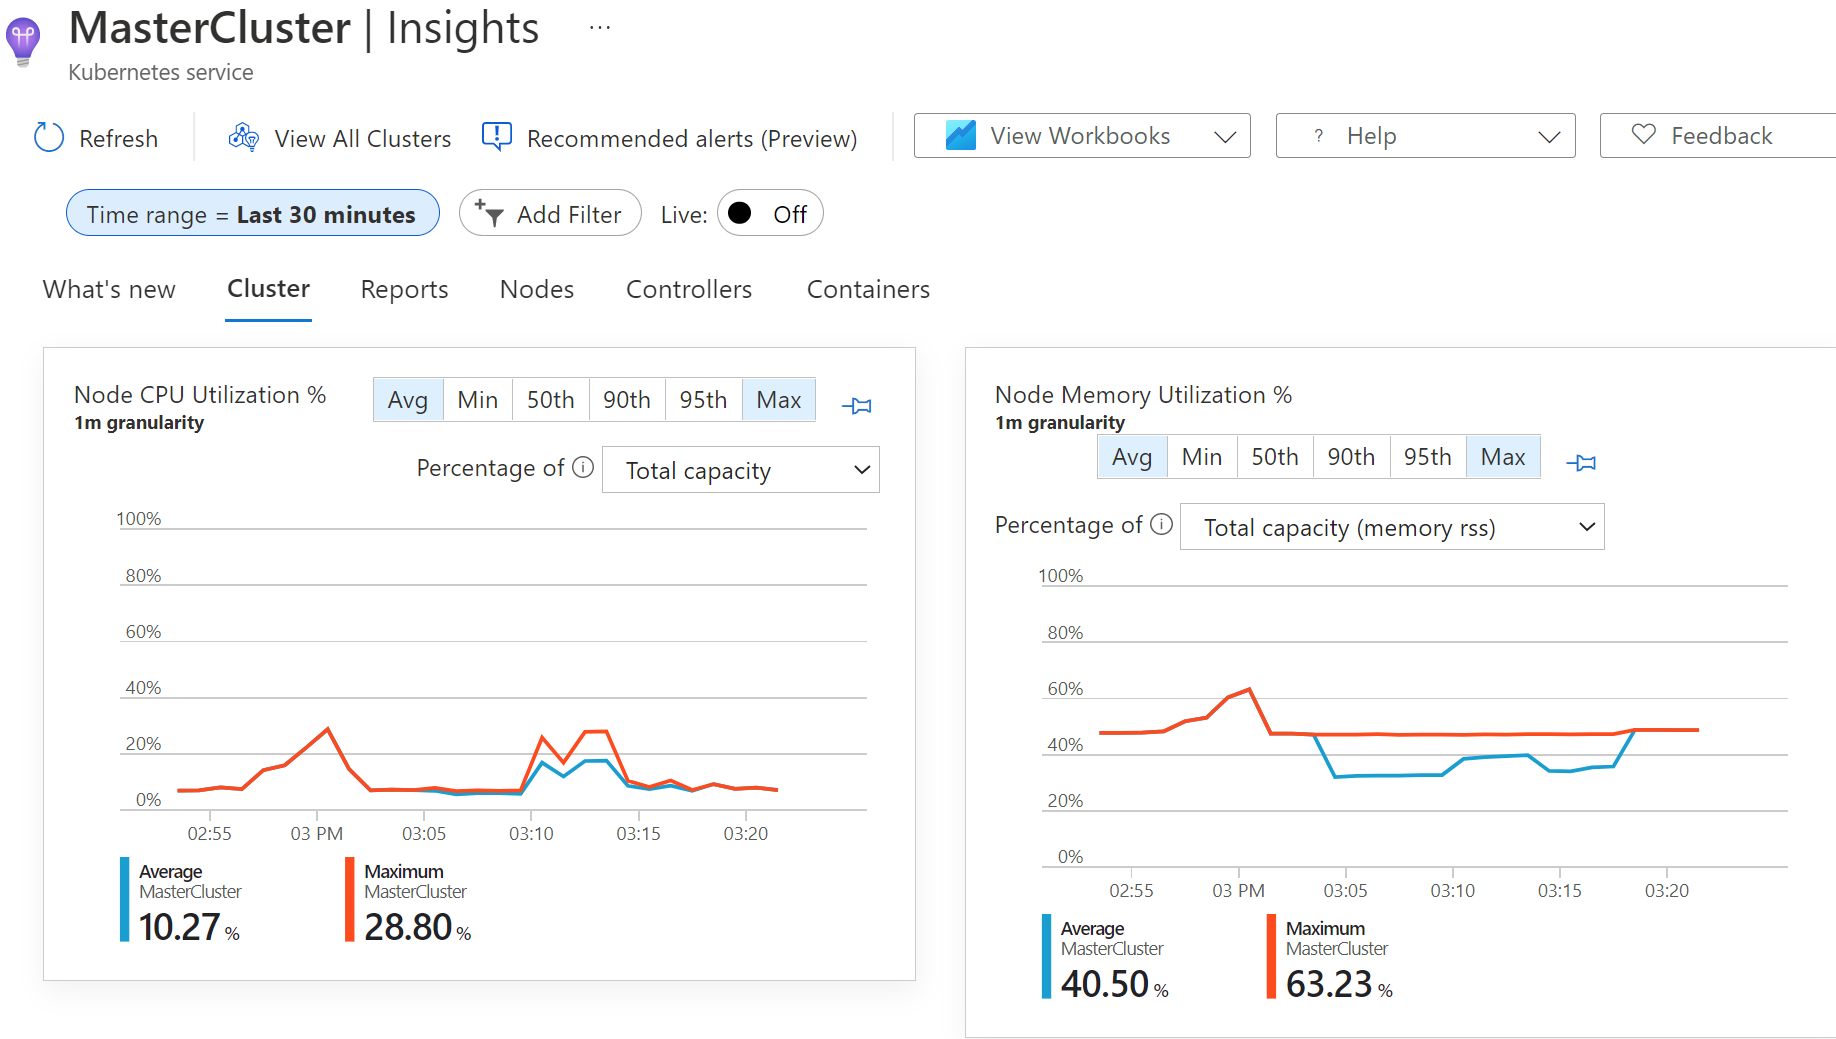
\includegraphics[width=1\textwidth]{./images/aks_insights.png}}
  \caption{Pregled metrika klastera}
  \label{fig:aksinsights}
\end{figure}

Na slici \ref{fig:clusterunhealthy} je prikazan pregled pokrenutih servisa na klasteru.
% Na slici se vidi da je servis markiran uzvičnikom, jer nije dostignut željeni broj zdravih replika (0\% replika je zdravo).

\begin{figure}[!ht]
  \centering
  \frame{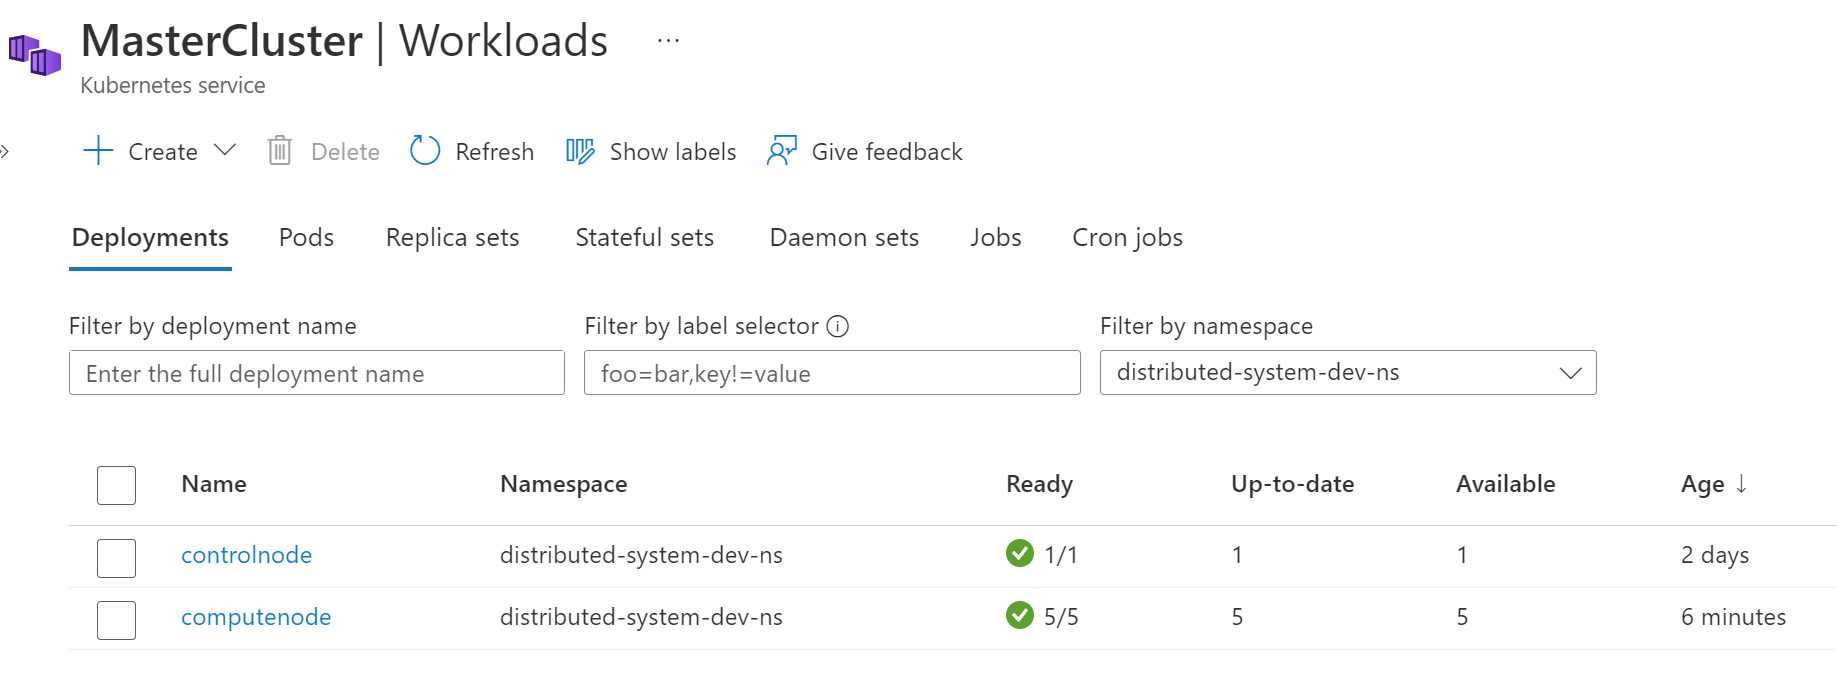
\includegraphics[width=1\textwidth]{./images/metrics_cluster.png}}
  \caption{Pogled na metrike o statusu klastera}
  \label{fig:clusterunhealthy}
\end{figure}

\subsection{Logovi}

Logovi predstavljaju informacije o radu sistema koje ispisuju pokrenuti servisi u tekstualnom formatu. Oni su automatski sakupljeni sa mašina i prosleđeni na mesto za čuvanje, gde im je moguće pristupiti kroz propratne alate.

Za pregled logova korišćen je alat \emph{Azure Log Analytics} dostupan u okviru servisa \emph{Azure Monitor}. Ovaj alat pruža moćan deskriptivni jezik kojim se mogu pretraživati, filtrirati, sortirati i analizirati logovi. Rezultate upita je takođe moguće vizuelizovati u vidu grafikona.

Na slici \ref{fig:computenodelogs} se nalazi prikaz stranice za pregled logova kontejnera koji sadrži aplikaciju \emph{Control Node}.

\begin{figure}[!ht]
  \centering
  \frame{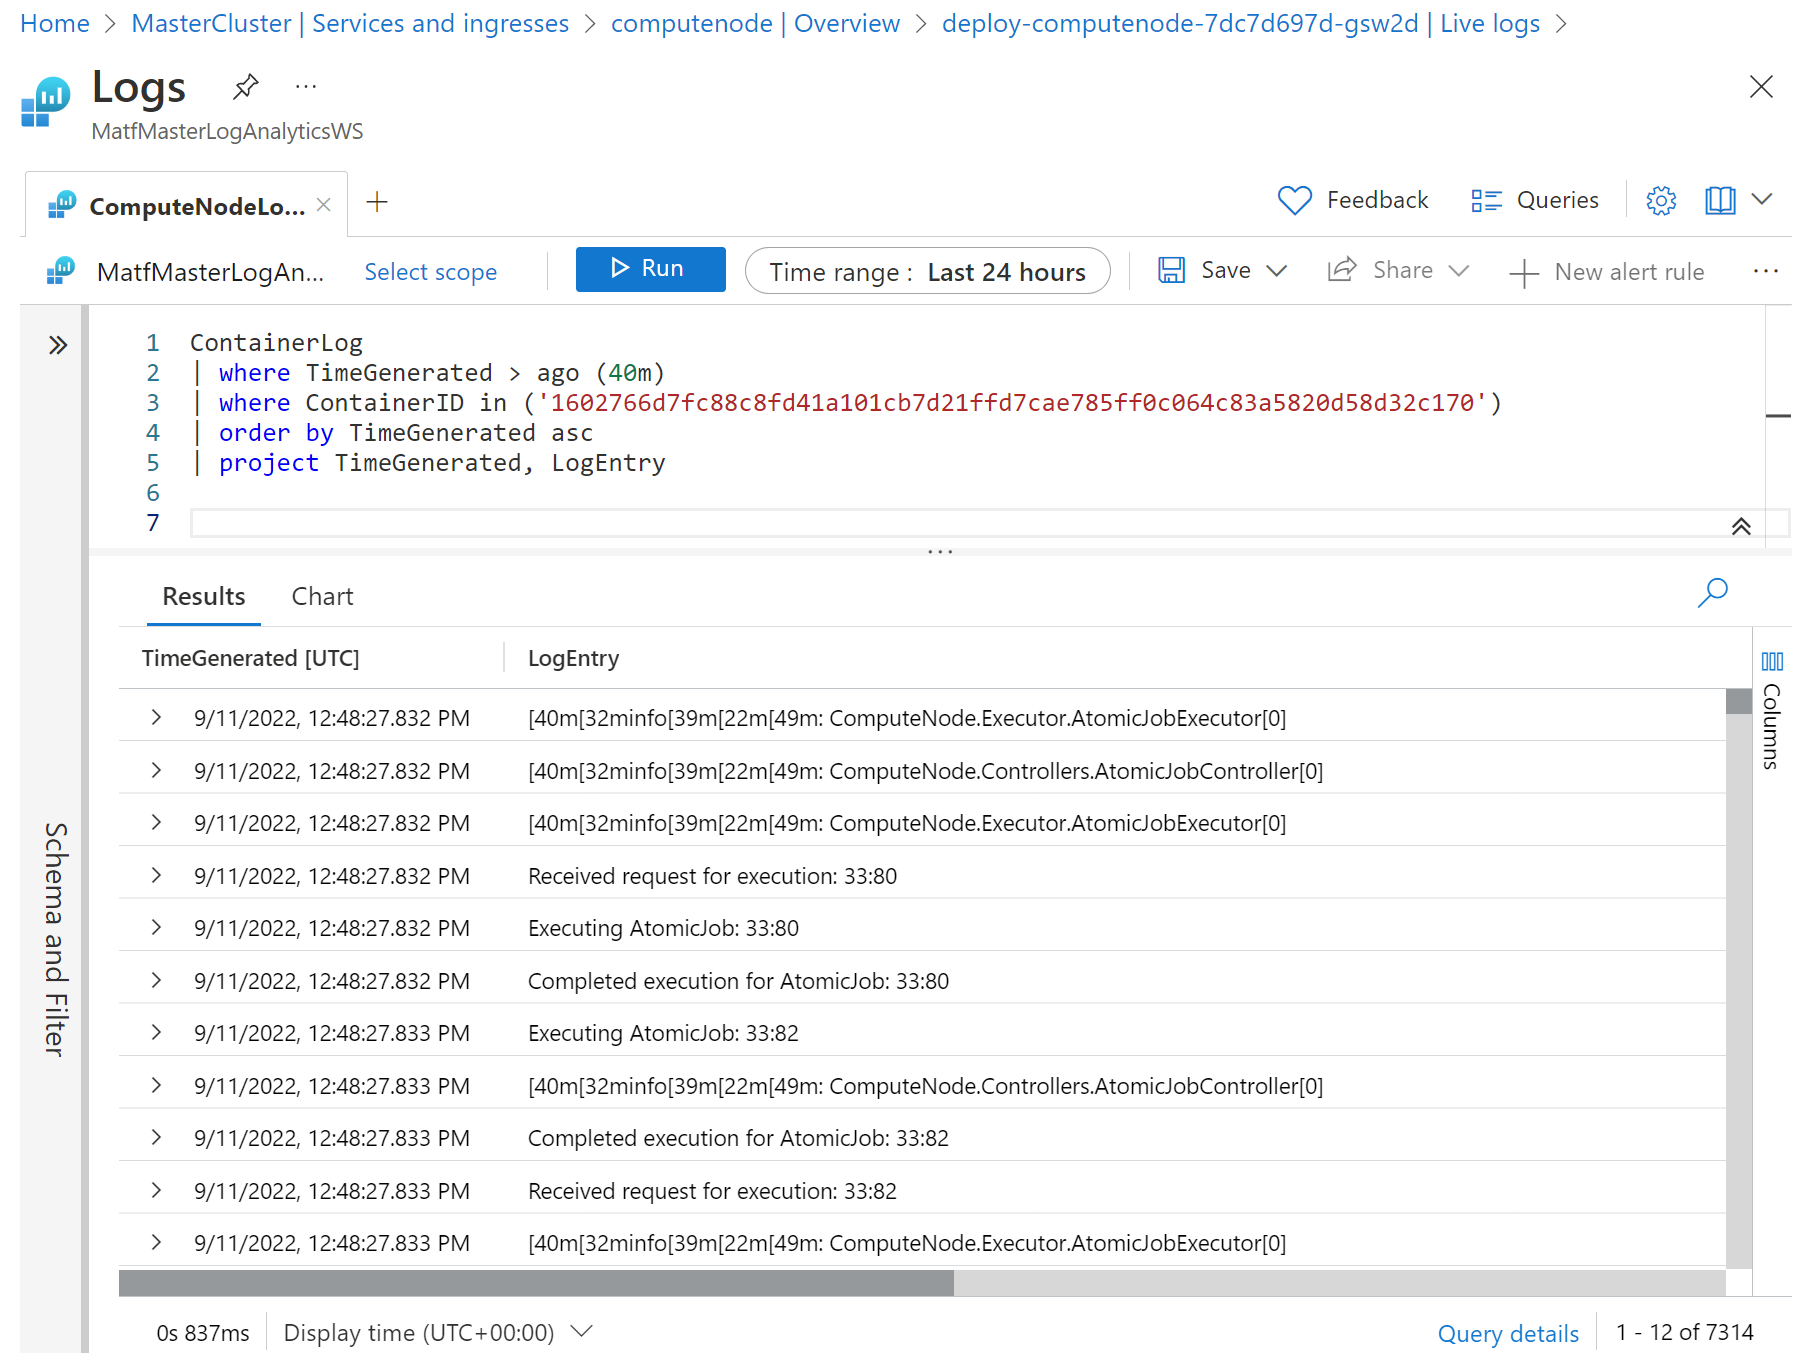
\includegraphics[width=1\textwidth]{./images/computenode_logs.png}}
  \caption{Pregled logova komponente \emph{Compute Node}}
  \label{fig:computenodelogs}
\end{figure}

Na slici \ref{fig:succeeded_vs_failed_jobs} se nalazi metrika o broju uspešnih i neuspešnih izvršenih poslova u periodu od sat vremena, agregiranih na 10 minuta.

\begin{figure}[!ht]
  \centering
  \frame{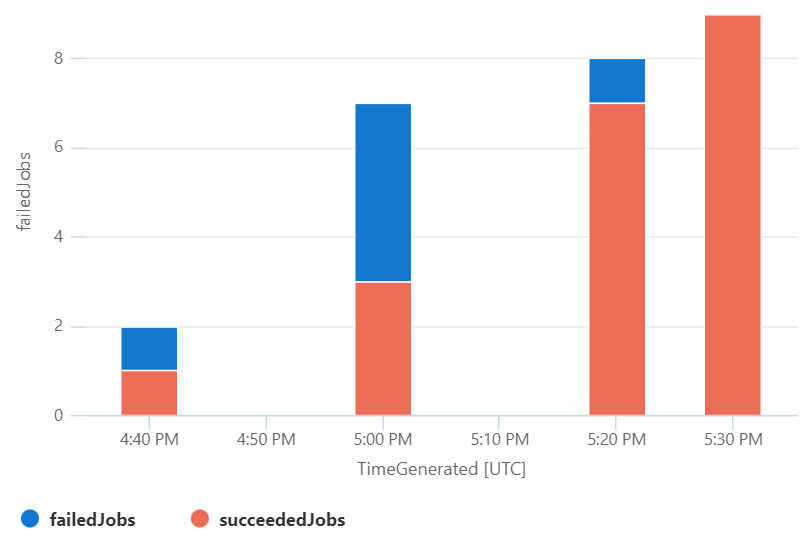
\includegraphics[width=0.7\textwidth]{./images/succeeded_failed_jobs.png}}
  \caption{Metrika o broju uspešnih i neuspešnih poslova kroz vreme}
  \label{fig:succeeded_vs_failed_jobs}
\end{figure}

\subsection{Uzbunjivači}

Korisnik koji ima pravo pristupa logovima i metrikama može da napravi automatsku uzbunu (eng. \emph{Alert}) u nekim situacijama od značaja. Ovaj servis periodično proverava dostupne metrike i logove, i proverava da li su se ispunjeni uslovi definisani tokom njegovog kreiranja. Ukoliko zaključi da postoji problem, podiže uzbunu na ranije definisan način (mejlom, SMS-om, pozivom, obaveštenjem) i, ukoliko postoje, automatski pokreće definisane akcije. Problemi u produkcionom okruženju se javljaju, i u tim slučajevima je cilj što pre reagovati i obezbediti da sistem bude zdrav i na raspolaganju korisnicima.

U nastavku se na slici \ref{fig:alertex} nalazi primer aktivnog upozoranja u slučaju grešaka koje bacaju komponente sistema.

\begin{figure}[!ht]
  \centering
  \frame{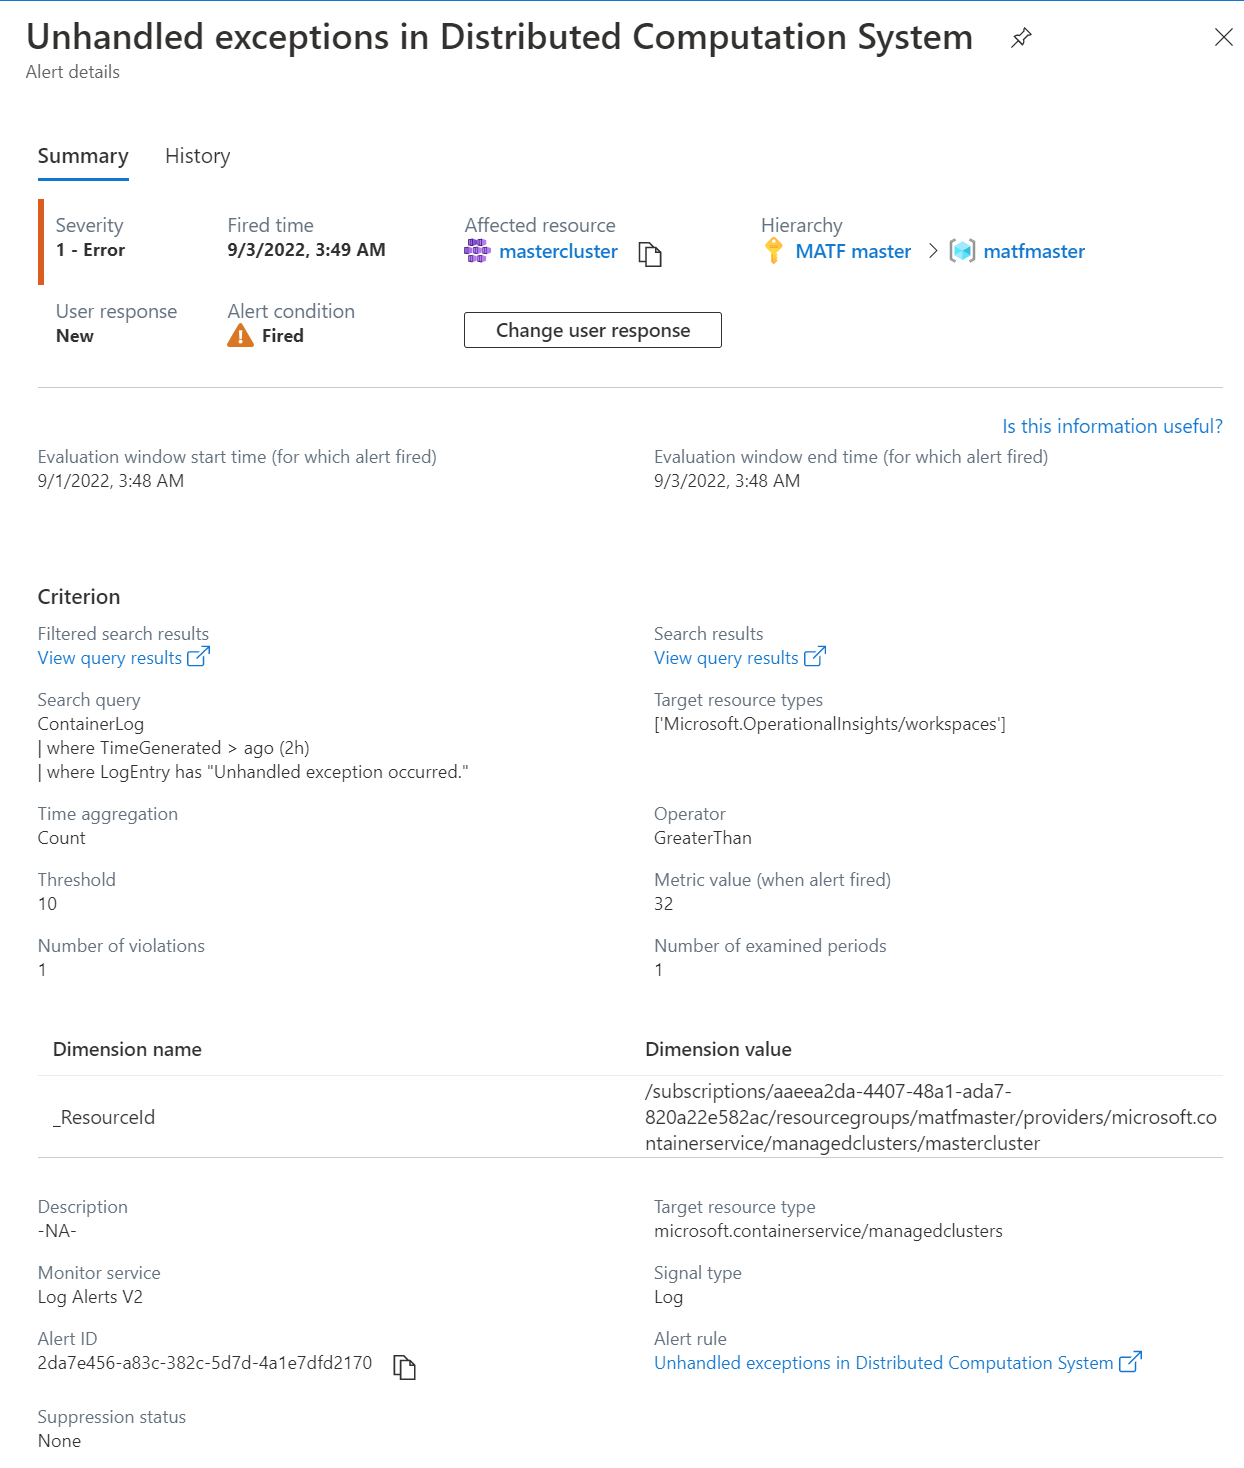
\includegraphics[width=1\textwidth]{./images/alert_unhandled_exceptions.png}}
  \caption{Aktivni uzbunjivač u slučaju neočkivanih grešaka prisutnim u logovima kontejnera}
  \label{fig:alertex}
\end{figure}

Na slici \ref{fig:alertmemory} nalazi primer aktivnog opšteg upozorenja u slučaju nedostatka memorije na mašinama. Analogno, postoji i uzbunjivač koji prati procenat iskorišćenosti dostupnog procesora.

\begin{figure}[!ht]
  \centering
  \frame{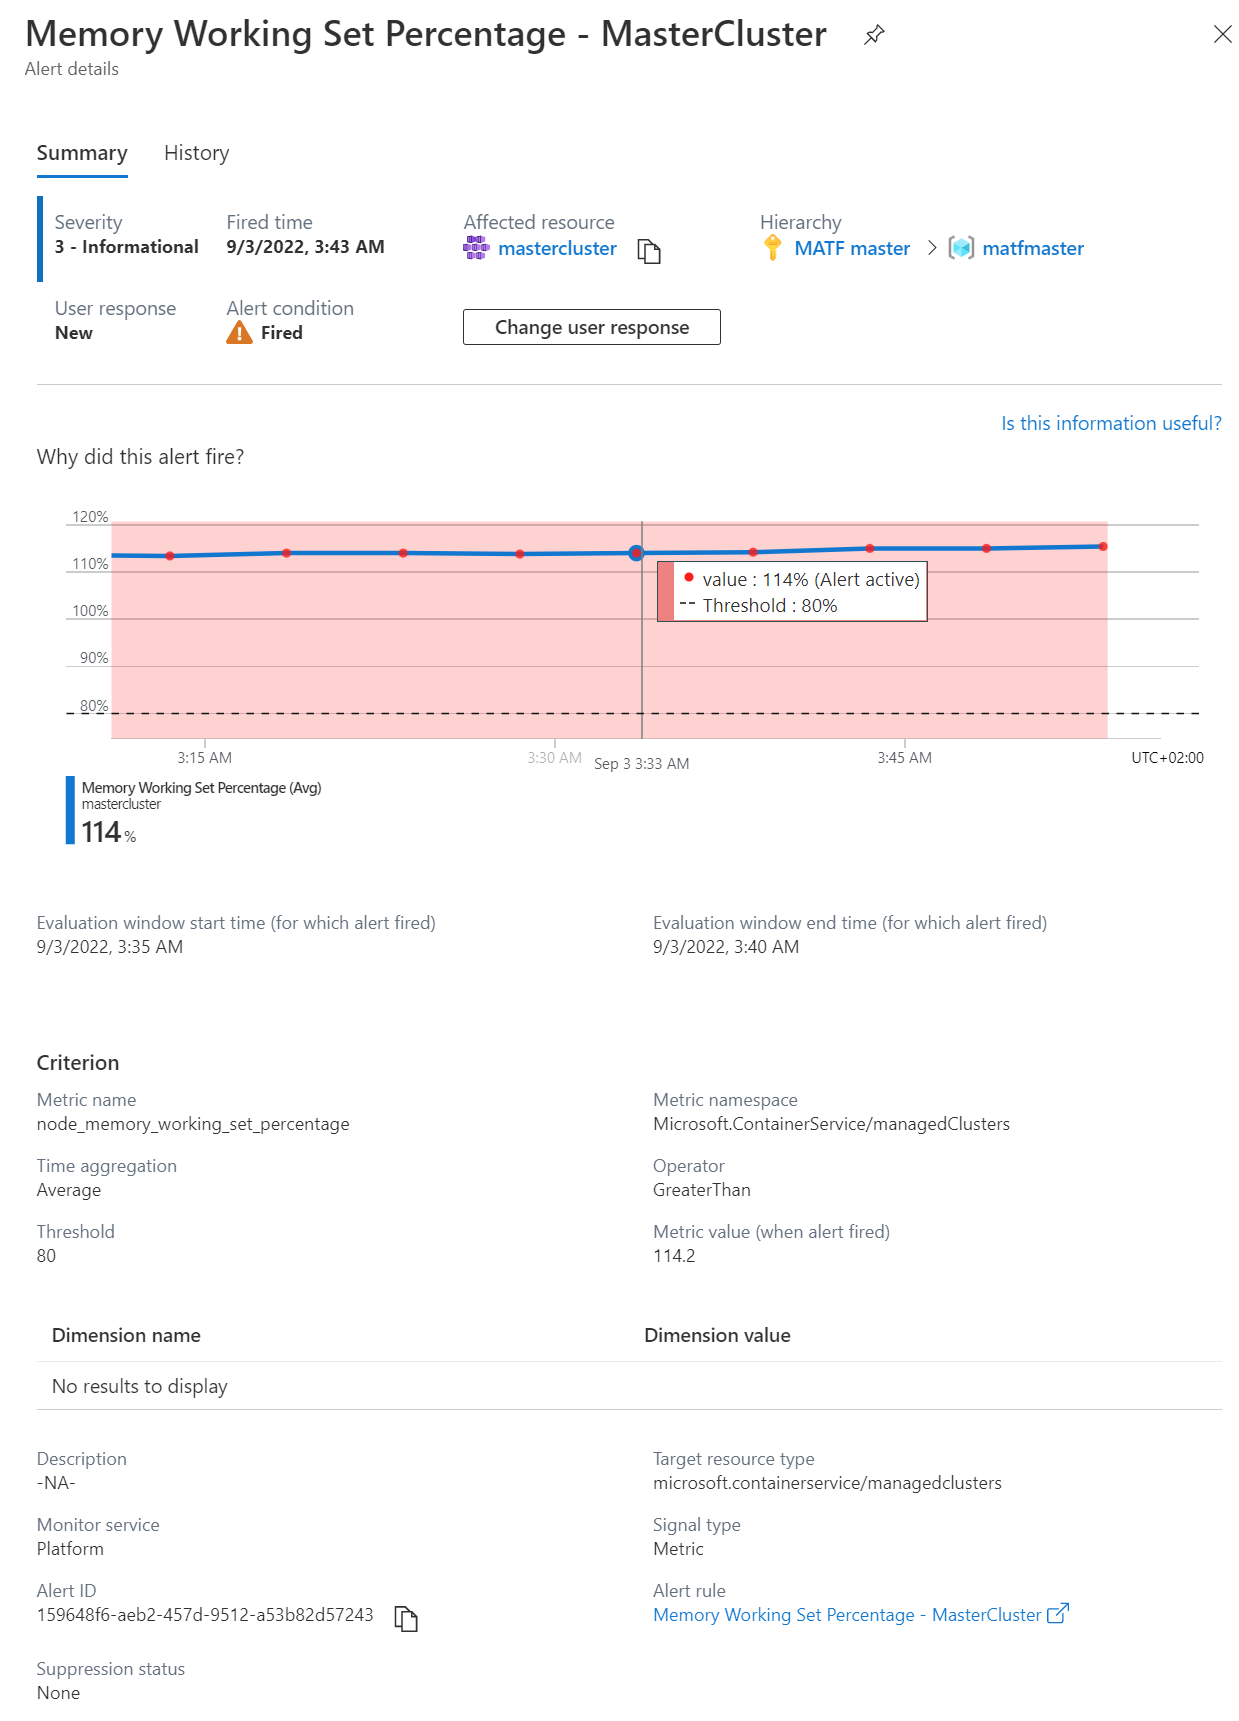
\includegraphics[width=1\textwidth]{./images/alert_memory_pressure.png}}
  \caption{Uzbunjivač u slučaju nedovoljno memorije u klasteru}
  \label{fig:alertmemory}
\end{figure}


% ------------------------------------------------------------------------------
\chapter{Rezultati}
\label{chp:rezultati}
% ------------------------------------------------------------------------------

\section{Implementirani poslovi}

Prva verzija sistema DCS implementira \emph{map-reduce} funkcionalnost nad nizom brojeva. Rezultat izračunavanja je ukupan zbir cifara brojeva od 1 do svakog elementa niza pojedinačno. Svaki element niza predstavlja jedan ulazni podatak za atomični posao. Ovaj primer veštački pravi zahtevan posao koji treba obraditi, ali je dovoljan da dokaže koncept i smislenost sistema.

\emph{Primer.}

Ulazni niz: [11, 3, 1]

Izlaz: 55 = (1 + 2 + 3 + 4 + 5 + 6 + 7 + 8 + 9 + (1 + 0) + (1 + 1)) + (1 + 2 + 3) + (1)

Otkazivanje zakazanih poslova nije podržano u inicijalnoj verziji.

\section{Analiza performansi}

Za ispitivanje performansi sistema, izvršeno je merenje dužine trajanje obrade posla u nekoliko okruženja: sekvencijalno na jednoj mašini, nad klasterom u oblaku koji se sastoji od 1, 5, odnosno 10 jedinica za izračunavanje. Rezultati su prikazani u tabeli \ref{tbl:rezultati}. Veličina ulaza predstavlja broj elemenata niza generisanih na slučajan način. Generisani brojevi se nalaze u rasponu od 400000 do 450000. Ovaj raspon je izabran empirijski, jer se nad velikim brojevima primećuje dovoljno povećanje vremena izvršavanja. Rezultati merenja su predstavljeni u sekundama, zaokruženi na drugu decimalu. Rezultati merenja so prosečna vrednost nakon tri pokretanja izračunavanja sa istim ulaznim podacima.

\begin{table}
\centering
\begin{center}
\begin{tabular}{ |c||c|c|c|c| } 
 \hline
  veličina ulaza & lokalno, sekvencijalno & DCS 1 cmpN & DCS 5 cmpN & DCS 10 cmpN \\ 
 \hline
 50 & 1.09 & 0.37 & 0.42 & 0.41 \\ 
 100 & 2.36 & 0.81 & 0.63 & 0.67 \\ 
 500 & 12.05 & 3.97 & 2.99 & 3.12 \\ 
 1000 & 23.6 & 8.23 & 6.39 & 6.74 \\ 
 3000 & 78.16 & 29.17 & 24.12 & 25.84 \\ 
 \hline
\end{tabular}
\caption{Rezultati izvršavanja u različitim okruženjima}
\label{tbl:rezultati}
\end{center}
\end{table}

Iz navedenih rezultata se vidi poboljšanje vremena izvršavanja. Dodavanjem jedinica za izvršavanje, smanjuje se vreme izvršavanja. Ovo je i očekivano, s obzirom na povećanje nivoa paralelizma. Međutim, dodavanje jedinica za izvršavanje može da ubrza izvršavanje do određene granice. Iz rezultata se vidi da je vreme izvršavanja, prilikom pokretanja poslova nad sistemom sa 5, odnosno 10 jedinica za izvršavanje, veoma slično.

U prvoj iteraciji testiranja performansi, poboljšanje nije bilo veliko koliko bi se očekivalo, u poređenju sa lokalnim, sekvencijalnim pokretanjem algoritma. Korišćen je klaster sa ograničenim resursima. Klaster u oblaku ima ograničenja poput količine podataka i zahteva koji se propuštaju kroz mrežu, i to usporava rad sistema. Takođe, i pripadajuća baza podataka ima ograničenja potrošnje resursa i broja zahteva koje obrađuje, te može početi da odbija zahteve koji dolaze od DCS. Kada je klasteru i bazi podataka dodeljena veća količina resursa, rezultati su se primetno poboljšali. Ovo ide u prilog skalabilnosti sistema, jer su se, kroz jednostavne konfiguracione promene, dobili bolji rezultati.

\section{Dalji razvoj sistema}

Predloženo je nekoliko ideja u kojem pravcu bi sistem DCS mogao da se razvija. Neki od pravaca daljeg razvoja su:
\begin{enumerate}
\item Generalizacija tipa poslova,
\item Podrška za različite frontende,
\item Napredno rutiranje zahteva ka jedinicama za izvršavanje.
\end{enumerate}

Pored navedenih mogućnosti, sistem bi mogao da preusmeri pisanje rezultata na proizvoljnu lokaciju, na osnovu tipa posla. Ukoliko su ulazni podaci ili rezultat veliki, te ih nije praktično čuvati u bazi podataka, DCS je moguće proširiti kako bi koristio neko drugo skladište za pristup ulaznim podacima i za čuvanje rezultata.

\subsection{Generalizacija tipa poslova}

Prikazani sistem u inicijalnoj implementaciji može da obrađuje samo poslove koji se sastoje od niza atomičnih poslova. Dodavanje podrške za obradu novih tipova poslova je moguća uz sitnije izmene, čija je suština u dodavanju klase koja izvršava specifični atomični posao. Ova klasa implementira \href{https://github.com/milana-kovacevic/DistributedComputationSystem/blob/main/src/ComputeNode/Executors/ISpecificJobExecutor.cs}{\emph{ISpecificJobExecutor} interfejs} u projektu jedinice za izvršavanje. Izbor tipa posla koji bi sledeći bio implementiran, zavisi od potražnje na tržištu.

Potpunu generalizaciju obrade atomičnih jedinica posla moguće je izvesti proširivanjem korisničkog interfejsa za zakazivanje posla, tj. proširenjem interfejsa tako da mu ulazni parametar bude izvorni kod funkcije koju je potrebno izvršiti nad atomičnim poslovima. Tada bi korisnik, pored ulaznih podataka, prosledio i deo koda koji želi da se izvrši nad atomičnim poslovima na sistemu. Za podršku ovog slučaja upotrebe, potrebno je da sistem zna da prevede izvorni kod funkcije i rezultujuću funkciju prosledi jedinici za izvršavanje. Ovaj pristup podrazumeva bezbednosne provere unetog koda, kako bi se osigurali od napada na klaster. Razvoj sistema u ovom pravcu bi naginjao ka postojećem rešenju \emph{Azure Functions} spomenutog u odeljku \ref{sub:postojeca_resenja} pod rednim brojem \ref{azurefunctions}.

Dalja unapređenja bi mogla da uključe obradu poslova koji nisu nužno specificirani nizom svojih atomičnih podjedinica. Ovo podrazumeva da programer razume suštinu izvršavanja novog tipa posla, te generiše plan za distribuirano izvršavanje. Kompleksni posao od korisnika bi prvo trebalo podeliti na više manjih, dok plan izvršavanja može da uključuje i agregaciju podrezultata zbog eventualnih zavisnosti potposlova. Razvoj sistema u ovom pravcu bi naginjao ga sistemima poput Sparka \cite{Spark} spomenutog u odeljku \ref{sub:postojeca_resenja}.

\subsection{Podrška za različite frontende}

U okviru implementirane kontrolne jedinice, komponenta \emph{Frontend} daje korisniku na korišćenje \emph{REST API}. Dalji razvoj servisa bi mogao da podrži i druge klijent - server načine komunikacije, uključujući komunikaciju preko \emph{Web Socketa}. Takođe, moguće je izraditi \emph{Web} platformu i vizuelni korisnički interfejs za lakše korišćenje sistema.

Sistem je moguće proširiti, tako da uključuje podršku i za druge tipove autentifikacije. Osnovna autentikacija uključuje integrisanje sa provajderom identiteta \emph{Azure Active Directory}. Ovo je moguće unaprediti dodavanjem odvojene komponente za podršku za druge načine autentifikacije (na primer, koriščenjem \emph{Google} naloga).

Navedena poboljšanja bi dodatno opteretila postojeću implementaciju kontrolne jedinice. Sa daljim razvojem u ovom delu servisa, trebalo bi razdvojiti implementaciju \emph{Frontend} servisa od orkestratora distribuiranja, i nastaviti razvoj imajući u vidu pristup razvijanja kroz mikro-servise. To bi uključilo izradu drugih \emph{Frontend} servisa koji bi komunicirali sa svojim klijentima, a poslove slali na centralni servis zadužen za distribuirano orkestriranje.


\subsection{Napredno rutiranje zahteva ka jedinicama za izvršavanje}

Urađena implementacija se, prilikom izvršavanja atomičnih jedinica posla na jedinicama za izvršavanje, oslanja na Kubernetes podršku za balansiranje zahteva koji idu kroz mrežu do servisa. Drugi, samostalniji način zakazivanja poslova bi uključio prepoznavanje adresa jedinica za izvršavanje (tj. njihovih mahuna), a zatim bi tu informaciju iskoristio za proizvoljno, pametnije usmeravanje poslova na izvršavanje na tim adresama. U kalkulacije bi uključio i procene kompleksnosti posla, kao i dostupne resurse.

Ova implementacija je zahtevnija, ali pruža priliku za bolje performanse. Međutim, pre početka same implementacije, potrebno je izvršiti opsežno testiranje i analiziranje postojućeg sistema kako bi se opravdala potreba za novim orkestratorom distribuiranog izvršavanja. Ukoliko osnovna varijanta algoritma za orkestriranje ne zadovoljava kriterijume performansi, onda ima smisla raditi ovakva unapređenja.

Ukoliko je unapređenje opravdano, za početak, potrebno je napraviti infrastrukturu za pronalaženje adresa u okviru komponente koja vrši zakazivanje poslova. Dodatno, treba implementirati algoritam koji procenjuje kompleksnost posla u vidu potrebnih resursa za njegovo izračunavanje. Na kraju, potrebno je i implementirati novi orkestrator. Nakon svega ovoga, potrebno je uraditi testiranje sistema sa novom implementacijom, kao i testiranje \emph{AB} sistema kako bi se doneli zaključci koji je princip bolji i zašto.

\section{Zaključak}
U radu je predstavljen sistem za dristribuirano izračunavanje DCS. Opisani su detalji sistema, što uključuje mehanizam za primanje zahteva za obradu poslova, zakazivanje posla, distribuirano izvršavanje i praćenje poslova. Opisan je način praćenja rada sistema, kao i načini njegovog testiranja.

Nadogradnje sistema ne zahtevaju veću refaktorizaciju, jer je sistem projektovan da bude modularan, uspostavljajući svu potrebnu infrastrukturu. Ovo čini da se sistem može lako proširiti, kako bi uveo dodatne funkcionalnosti za obradu novih tipova poslova. Postojeći sistem implementira jednostavnu funkcionalnost, kako bi predstavio prednosti predloženog pristupa.

Implementirani sistem DCS pokazuje značajno ubrzanje u odnosu na izvršavanje na jednoj mašini. Pokretanjem sistema u oblaku, on je veoma skalabilan i prilagodljiv potrebama korisnika. Kako bi se dostigle najbolje perfomanse sistema za određeni tip poslova, potrebno je prilagoditi konfiguraciju sistema i njegovih komponenti izvršavanju poslova od interesa.

Postoji više pravaca u kojem je moguće dalje razvijati sistem, a za definisanje pravog pravca je potrebno izvršiti ispitivanja potreba korisnika i tržišta. Na osnovu analiza dostupnih metrika i logova, moguće je doneti odluke u koje delove sistema je potrebno ulagati kako bi se dodatno poboljšale performanse.

% ------------------------------------------------------------------------------
% Literatura
% ------------------------------------------------------------------------------
\literatura

% ==============================================================================
% Završni deo teze i prilozi
\backmatter
% ==============================================================================

% ------------------------------------------------------------------------------
% Biografija kandidata
\begin{biografija}
  \textbf{Milana Kovačević} je rođena u Zrenjaninu, 29. novembra 1995. godine. Osnovno i srednje obrazovanje (Zrenjaninska gimnazija, prirodno-matematički smer) završila je u rodnom gradu, uz sticanje diplome "Vuk Karadžić". Takođe je završila nižu muzičku školu, instrument klavir.
2014. godine je upisala osnovne studije na modulu Informatika na Matematičkom fakultetu Univerziteta u Beogradu. Osnovne studije je završila 2017. godine sa prosečnom ocenom 9.86, kao primalac stipendije Dositeja. Master akademske studije je upisala 2017. godine, takođe na Matematičkom fakultetu na modulu Informatika. Položila je sve ispite predviđene planom i programom master akademskih studija sa prosečnom ocenom 9.15.

Nakon završetka osnovnih studija, nastavlja da se paralelno razvija i u industriji, radom u kompaniji \emph{Microsoft}. Tokom rada se susreće sa sistemima za obradu i čuvanje podataka u okviru platforme \emph{Azure}, a radom na jednom od njih, stiče i praktično znanje o distribuiranim sistemima i tehnologijama za rad u oblaku.

\end{biografija}
% ------------------------------------------------------------------------------

\end{document}
